\documentclass[UTF8,no-math,12pt,openany,table,dvipsnames,svgnames]{book}
\usepackage{etex,ctex}
\usepackage{manfnt}
\usepackage{textgreek}\usepackage{mathrsfs}
\usepackage{indentfirst}
\usepackage{fontspec}\usepackage{mathdesign}
\usepackage[T1]{fontenc}\usepackage{zhnumber}
\usepackage[centering,
           top=2.54cm,bottom=2.54cm,right=2.9cm,left=2.9cm,
           headsep=25pt,headheight=20pt]{geometry}
\usepackage[lite,zswash]{mtpro2}
\usepackage{amsmath,amsthm}\usepackage{autobreak}
\usepackage{cases}
%\usepackage{minitoc}%插入章节
%\dominitoc
\usepackage{extarrows}\newcommand{\hyds}[1]{{\CJKfontspec{汉仪大宋简}#1}}
\usepackage{graphicx}\usepackage{float}
\usepackage[perpage]{footmisc}
\usepackage{pgf,tikz,pgfplots}
\pgfplotsset{compat=1.14}
\usepackage{mathrsfs}\usepackage{pifont}
\usetikzlibrary{arrows}

\usepackage{enumerate}\usepackage{titlesec}
\usepackage{ulem}\renewcommand\rmdefault{ptm}
\usepackage[hyperindex]{hyperref}
\hypersetup{bookmarksopen=true,bookmarksopenlevel=1,bookmarksnumbered=true,
  pdftitle={平面几何集锦},pdfauthor={向禹},linktoc=page,
  colorlinks,linkcolor=blue,citecolor=red,urlcolor=blue,anchorcolor=green}
\usepackage[Symbol]{upgreek}
\renewcommand{\pi}{\uppi}
%\includeonly{章节文件名字}

%\usepackage{syntonly}\syntaxonly
\DeclareSymbolFont{ugmL}{OMX}{mdugm}{m}{n}
\SetSymbolFont{ugmL}{bold}{OMX}{mdugm}{b}{n}
\DeclareMathAccent{\wideparen}{\mathord}{ugmL}{"F3}

\setCJKmainfont[BoldFont={方正黑体_GBK},ItalicFont={方正楷体_GBK}]{方正书宋_GBK}

\defaultfontfeatures{Mapping=tex-text}
\XeTeXlinebreaklocale ”zh”
\XeTeXlinebreakskip = 0pt plus 1pt

\setCJKfamilyfont{song}{方正书宋_GBK}
\newcommand{\song}{\CJKfamily{song}}
\setCJKfamilyfont{hei}{方正黑体_GBK}
\newcommand{\hei}{\CJKfamily{hei}}
\setCJKfamilyfont{kai}{方正楷体_GBK}
\newcommand{\kai}{\CJKfamily{kai}}
\setCJKfamilyfont{fs}{方正仿宋_GBK}
\newcommand{\fs}{\CJKfamily{fs}}
\setCJKfamilyfont{fzxk}{方正行楷_GBK}
\newcommand{\fzxk}{\CJKfamily{fzxk}}
\setCJKfamilyfont{fzqt}{方正启体简体}
\newcommand{\fzqt}{\CJKfamily{fzqt}}
\newenvironment{Proof}{\par\noindent{\hei 证明}\hspace{1em}\setlength{\parindent}{2em}}{\par}
\newenvironment{solve}{\par\noindent{\hei 解}\hspace{1em}\setlength{\parindent}{2em}}{\par}
%\renewcommand{\dis}{\displaystyle}
\newtheorem{lemma}{引理}
\newtheorem{theorem}{定理}
\newtheorem{cor}{推论}
\newtheorem{example}{}
%\usepackage[toc,lof]{multitoc}\usepackage{xcolor,colortbl}
\everymath{\displaystyle}

\renewcommand{\le}{\leqslant}
\renewcommand{\ge}{\geqslant}

\allowdisplaybreaks[4]
\newcommand{\bd}{\boldsymbol}
%\numberwithin{equation}{section}

%--------将句号换成句点
%\catcode`\。=\active
%\newcommand{。}{.}\newcommand{\dis}{\displaystyle}\newcommand{\rank}{\mathrm{rank}}


\renewcommand{\qedsymbol}{\ding{73}}
\DeclareMathOperator{\tr}{tr}

\usepackage[most]{tcolorbox}
\usepackage{varwidth}
\newtcolorbox{MYBOX}[2][]{breakable,skin=enhancedlast jigsaw,before skip=2mm,enhanced,
after skip=2mm,colback=blue!5,colframe=blue!50,boxrule=0.2mm,sharp corners,
attach boxed title to top left={xshift=0.29cm,yshift*=1mm-\tcboxedtitleheight},
varwidth boxed title*=-3cm,
boxed title style={frame code={
   \path[fill=tcbcolback!30!black]
     ([yshift=-1mm,xshift=-1mm]frame.north west)
       arc[start angle=0,end angle=180,radius=1mm]
     ([yshift=-1mm,xshift=1mm]frame.north east)
       arc[start angle =180,end angle=0,radius=1mm];
     \path[left color=tcbcolback!60!black,right color=tcbcolback!60!black,
      middle color=tcbcolback!80!black]
      ([xshift=-2mm]frame.north west) -- ([xshift=2mm]frame.north east)
      [rounded corners=1mm]-- ([xshift=1mm,yshift=-1mm]frame.north east)
      -- (frame.south east) -- (frame.south west)
      -- ([xshift=-1mm,yshift=-1mm]frame.north west)
      [sharp corners]-- cycle;
      },interior engine=empty,
     },
     fonttitle=\bfseries,
     title={#2},#1}
\usepackage{fancyhdr,tikz}
\usetikzlibrary{shapes.callouts}
\renewcommand{\Re}{\operatorname{Re}}
\renewcommand{\Im}{\operatorname{Im}}
\newcommand{\ii}{\;\!\mathrm i\;\!}
\ctexset{punct=kaiming}
\renewcommand\thempfootnote{\ding{45}}
\newenvironment{note}{\par\CJKfamily{note}\noindent{\makebox[0pt][r]{\scriptsize\color{red!90}
\textdbend\quad}\textbf{注:}}}{\par}
\usepackage{tkz-euclide}

\pagestyle{fancy}
\fancyhf{}
\cfoot{\tikz\node[draw,cloud,cloud puffs=16,aspect=2,inner sep=0pt,fill=gray!20]{\thepage};}
\fancyhead[LO,RE]{\href{yuxtech.github.io}{我的博客: yuxtech.github.io}}
\fancyhead[RO,LE]{我的微信公众号: XiangMath}







\let\tkzTangent=\tkzDefTangent
\title{高中联赛难度平面几何习题集}
\author{向禹}
\usepackage{subfig}
\renewcommand\thesubfigure{\thefigure.\alph{subfigure}}
\usepackage[shortlabels]{enumitem}
\setlist{noitemsep,left=0cm}
%\renewcommand\bot{\perp}
	\newcommand\pxx{%
		\mathord{\text{\tikz[baseline] \draw[semithick] (0em,-0.3ex) -- ++(.4em,1.8ex) (.25em,-0.3ex) -- ++ (.4em,1.8ex);}%
	}}
\newcommand*\xs{%
		\mathrel{\text{%
				\tikz \draw[baseline,semithick] (-.25em,1.15ex) .. controls (-.55em,1.15ex) and (-.51em,.23ex) .. (-.275em,.23ex) .. controls (0,.23ex) and (0,1.15ex) .. (.275em,1.15ex) .. controls (.51em,1.15ex) and (.55em,.23ex) .. (.25em,.23ex);%
	}}}
	\newcommand*\quand{%
		\mathrel{\text{%\small%
				\tikz \draw[baseline,semithick] (-.2em,1.35ex) .. controls (-.46em,1.6ex) and (-.54em,.65ex) .. (-.25em,.65ex) .. controls (-.06em,.65ex) and (.06em,1.35ex) .. (.25em,1.35ex) .. controls (.54em,1.35ex) and (.46em,.4ex) .. (.2em,.65ex) (-.46em,.4ex) -- (.46em,.4ex) (-.46em,0ex) -- (.46em,0ex);%
	}}}
	\newcommand*\pxsbx{%
		\mathord{\text{%
				\tikz[baseline]
				\draw (0,.1ex) -- (.8em,.1ex) -- (1em,1.4ex) -- (.2em,1.4ex) -- cycle;}}}
	\newcommand*\qd{%
		\mathrel{\text{%\small%
				\tikz \draw[baseline] (-.2em,1.35ex) .. controls (-.46em,1.6ex) and (-.54em,.65ex) .. (-.25em,.65ex) .. controls (-.06em,.65ex) and (.06em,1.35ex) .. (.25em,1.35ex) .. controls (.54em,1.35ex) and (.46em,.4ex) .. (.2em,.65ex) (-.46em,.4ex) -- (.46em,.4ex) (-.46em,0ex) -- (.46em,0ex);%
	}}}
\tikzset{fuzhu/.style={densely dashed,draw=blue}}
\linespread{1.5}\selectfont
\begin{document}
\maketitle
\begin{enumerate}
\item 如图 \subref{1.1}, $P$为$\odot O$外一点, $PA,PB$分别切$\odot O$于$A,B,PCD$为$\odot O$的一条割线, $CD$交$\odot O$于另一点$E,AC,EB$交于点$F$,证明: $CD$平分$\angle ADF$.
\begin{figure}[!ht]
\centering
\subfloat[]{\label{1.1}
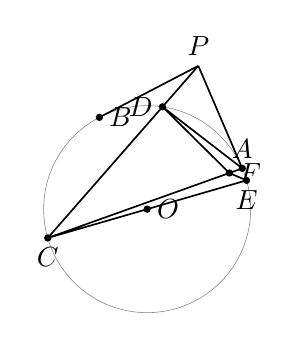
\begin{tikzpicture}[scale=0.65,semithick]
\tkzDefPoints{0/0/O,0.3/2/C,1/2.8/P}
\tkzDrawCircle(O,C)
\tkzTangent[from =P](O,C)\tkzGetPoints{A}{B}
\tkzInterLC(P,C)(O,C)\tkzGetPoints{D}{C}
\tkzInterLC(C,O)(O,C)\tkzGetPoints{C}{E}
\tkzInterLL(A,C)(E,B)\tkzGetPoint{F}
\draw[semithick](P)--(A)(D)--(A)(D)--(C)(P)--(C)(P)--(B)(D)--(F)
(E)--(C)(E)--(F)(A)--(C);
\tkzLabelPoints[above](A,P)
\tkzLabelPoints[left](D)
\tkzLabelPoints[right](B,O,F)
\tkzLabelPoints[below](E)
\tkzLabelPoints(C)
\tkzDrawPoints[size=2,fill=black](A,B,C,D,O,E,F)
\end{tikzpicture}
}
\subfloat[]{\label{1.2}
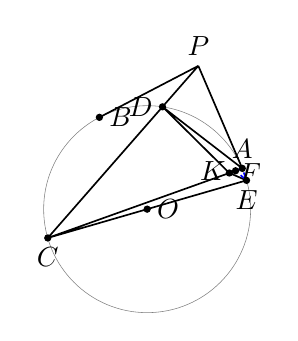
\begin{tikzpicture}[scale=0.65,semithick]
\tkzDefPoints{0/0/O,0.3/2/C,1/2.8/P}
\tkzDrawCircle(O,C)
\tkzTangent[from =P](O,C)\tkzGetPoints{A}{B}
\tkzInterLC(P,C)(O,C)\tkzGetPoints{D}{C}
\tkzInterLC(C,O)(O,C)\tkzGetPoints{C}{E}
\tkzInterLL(A,C)(E,B)\tkzGetPoint{F}
\tkzInterLL(C,A)(E,D)\tkzGetPoint{K}
\draw[semithick](P)--(A)(D)--(A)(D)--(C)(P)--(C)(P)--(B)(D)--(F)
(E)--(C)(E)--(F)(A)--(C);
\draw[densely dashed,blue,semithick](A)--(K)--(E)(E)--(A);
\tkzLabelPoints[above](A,P)
\tkzLabelPoints[left](D,K)
\tkzLabelPoints[right](B,O,F)
\tkzLabelPoints[below](E)
\tkzLabelPoints(C)
\tkzDrawPoints[size=2,fill=black](A,B,C,D,O,E,F,K)
\end{tikzpicture}
}
\subfloat[]{\label{1.3}
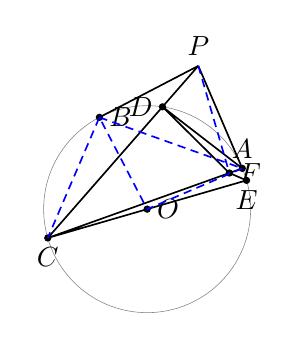
\begin{tikzpicture}[scale=0.65,semithick]
\tkzDefPoints{0/0/O,0.3/2/C,1/2.8/P}
\tkzDrawCircle(O,C)
\tkzTangent[from =P](O,C)\tkzGetPoints{A}{B}
\tkzInterLC(P,C)(O,C)\tkzGetPoints{D}{C}
\tkzInterLC(C,O)(O,C)\tkzGetPoints{C}{E}
\tkzInterLL(A,C)(E,B)\tkzGetPoint{F}
\draw[semithick](P)--(A)(D)--(A)(D)--(C)(P)--(C)(P)--(B)(D)--(F)
(E)--(C)(E)--(F)(A)--(C);
\tkzLabelPoints[above](A,P)
\tkzLabelPoints[left](D)
\tkzLabelPoints[right](B,O,F)
\tkzLabelPoints[below](E)
\tkzLabelPoints(C)
\tkzDrawPoints[size=2,fill=black](A,B,C,D,O,E,F)
\draw[densely dashed,blue,semithick](A)--(O)--(B)--(C)(B)--(A)(P)--(F);
\end{tikzpicture}
}
\caption{第 \thefigure 题图}
\end{figure}
\begin{Proof}
{\kaishu 方法一}\quad 如图 \subref{1.2}, 延长$ED$交$CA$于$K$,根据条件知四边形$CADB$为调和四边形,故$ED,EC,EA,EB$构成一组调和线束,进而知$K,C,A,F$构成一组调和点列.而$KD\bot CD$,故$CD$平分$\angle ADF$.

{\kaishu 方法二}\quad 如图 \subref{1.3},连接$OA,OB,AB,BC$,因为
\begin{align*}
\angle AFB&=\angle ACE-\angle BEC=\frac{\angle AOE-\angle BOC}2\\
&=\frac{180^\circ-\angle AOC-\angle BOC}2=\frac{\angle APC}2
\end{align*}
且$PA=PB$,故点$P$为$\triangle ABF$的外心.于是知$\angle PFA=\angle PAC=\angle PDA$,所以$P,A,D,F$四点共圆.由$PA=PF$,故$CD$平分$\angle ADF$.
\end{Proof}
\item 如图 \subref{2.1}, $AB$为$\odot O$的直径, $C,D$为$\odot O$上的两点,且在$AB$同侧, $\odot O$在$C,D$两处的切线交于点$E$, $BC,AD$交于点$F$, $EF$交$AB$于$M$,证明: $E,C,M,D$四点共圆.
\begin{figure}[!ht]
\centering
\subfloat[]{\label{2.1}
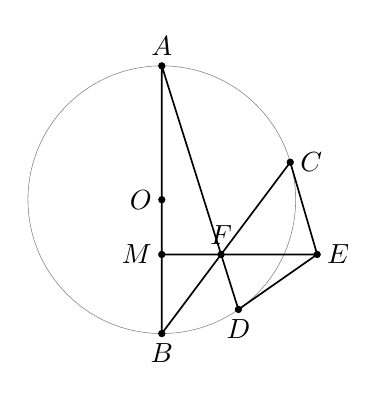
\begin{tikzpicture}[semithick,scale=0.85]
\begin{scope}[rotate=-90]
\tkzDefPoints{-2/0/A,2/0/B,0.4/0/K,0.8/0/K1}
\tkzDefMidPoint(A,B)\tkzGetPoint{O}
\tkzDrawCircle(O,A)
\tkzInterCC(A,K)(O,A)\tkzGetPoints{C}{C1}
\tkzInterCC(B,K1)(O,A)\tkzGetPoints{D1}{D}
\tkzTangent[at=C](O)\tkzGetPoint{C2}
\tkzTangent[at=D](O)\tkzGetPoint{D2}
\tkzInterLL(C,C2)(D,D2)\tkzGetPoint{E}
\tkzInterLL(A,D)(B,C)\tkzGetPoint{F}
\tkzInterLL(E,F)(A,B)\tkzGetPoint{M}
\end{scope}
\draw(A)--(B)--(C)--(E)--(D)--(A)(E)--(M);
\tkzLabelPoints[left](O,M)
\tkzLabelPoints[right](C,E)
\tkzLabelPoints[above](A,F)
\tkzLabelPoints[below](B,D)
\tkzDrawPoints[size=2,fill=black](A,O,B,C,E,D,F,M)
\end{tikzpicture}
}\hspace{2cm}
\subfloat[]{\label{2.2}
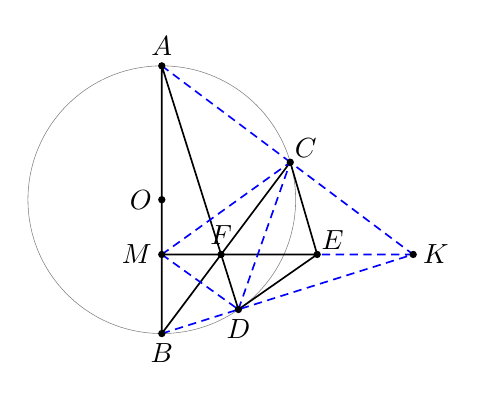
\begin{tikzpicture}[semithick,scale=0.85]
\begin{scope}[rotate=-90]
\tkzDefPoints{-2/0/A,2/0/B,0.4/0/K,0.8/0/K1}
\tkzDefMidPoint(A,B)\tkzGetPoint{O}
\tkzDrawCircle(O,A)
\tkzInterCC(A,K)(O,A)\tkzGetPoints{C}{C1}
\tkzInterCC(B,K1)(O,A)\tkzGetPoints{D1}{D}
\tkzTangent[at=C](O)\tkzGetPoint{C2}
\tkzTangent[at=D](O)\tkzGetPoint{D2}
\tkzInterLL(C,C2)(D,D2)\tkzGetPoint{E}
\tkzInterLL(A,D)(B,C)\tkzGetPoint{F}
\tkzInterLL(E,F)(A,B)\tkzGetPoint{M}
\tkzInterLL(A,C)(B,D)\tkzGetPoint{K}
\end{scope}
\draw(A)--(B)--(C)--(E)--(D)--(A)(E)--(M);
\draw[densely dashed,blue,semithick](M)--(C)--(K)--(D)--(M)(D)--(C)(K)--(E)
(A)--(C)(B)--(D);
\tkzLabelPoints[left](O,M)
\tkzLabelPoints[right](K)
\tkzLabelPoints[above right=-1mm](E,C)
\tkzLabelPoints[above](A,F)
\tkzLabelPoints[below](B,D)
\tkzDrawPoints[size=2,fill=black](A,O,B,C,E,D,F,M,K)
\end{tikzpicture}
}
\caption{第 \thefigure 题图}
\end{figure}

\begin{Proof}
如图 \subref{2.2}, 延长$AC,BD$交于点$K$,则$BC\bot AK,AD\bot BK$,从而知$F$为$\triangle KAB$的垂心.又在圆内接六边形$CCADDB$中使用帕斯卡定理,知$K,E,F$三点共线,从而$KM\bot AB$于$M$.于是有$\angle CMF=\angle CAF=\angle CDE$,所以$E,C,M,D$四点共圆.
\end{Proof}
\item 如图 \subref{3.1}, $AB$为$\odot O$的直径, $C,D$为$\odot O$上两点,且在$AB$同侧. $\odot O$在$C,D$两处的切线交于点$E,BC,AD$交于点$F,EB$交$\odot O$于点$G$,证明: $\angle CEF=2\angle AGF$.
\begin{figure}[!ht]\centering
\subfloat[]{\label{3.1}
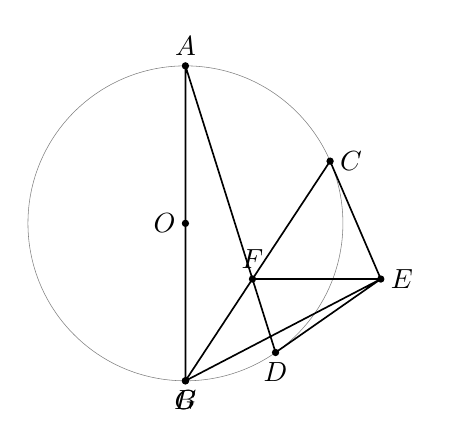
\begin{tikzpicture}[semithick]
\begin{scope}[rotate=-90]
\tkzDefPoints{-2/0/A,2/0/B,0.2/0/K,0.8/0/K1}
\tkzDefMidPoint(A,B)\tkzGetPoint{O}
\tkzDrawCircle(O,A)
\tkzInterCC(A,K)(O,A)\tkzGetPoints{C}{C1}
\tkzInterCC(B,K1)(O,A)\tkzGetPoints{D1}{D}
\tkzTangent[at=C](O)\tkzGetPoint{C2}
\tkzTangent[at=D](O)\tkzGetPoint{D2}
\tkzInterLL(C,C2)(D,D2)\tkzGetPoint{E}
\tkzInterLL(A,D)(B,C)\tkzGetPoint{F}
\tkzInterLC(E,B)(O,A)\tkzGetPoints{G}{B1}
\end{scope}
\draw(A)--(B)--(C)--(E)--(D)--(A)(E)--(F)(E)--(B)(A)--(G)--(F);
\tkzLabelPoints[left](O)
\tkzLabelPoints[right](C,E)
\tkzLabelPoints[above](A,F)
\tkzLabelPoints[below](B,D)
\tkzLabelPoints(G)
\tkzDrawPoints[size=2,fill=black](A,O,B,C,E,D,F,G)
\end{tikzpicture}
}\hspace{2cm}
\subfloat[]{\label{3.2}
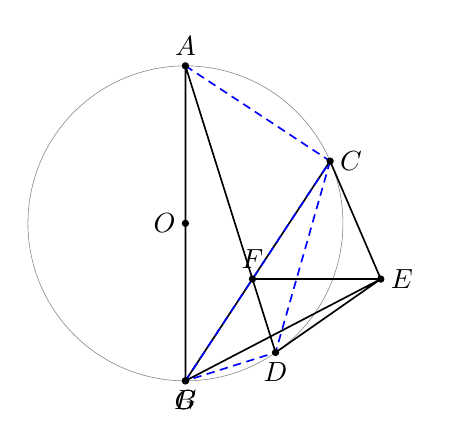
\begin{tikzpicture}[semithick]
\begin{scope}[rotate=-90]
\tkzDefPoints{-2/0/A,2/0/B,0.2/0/K,0.8/0/K1}
\tkzDefMidPoint(A,B)\tkzGetPoint{O}
\tkzDrawCircle(O,A)
\tkzInterCC(A,K)(O,A)\tkzGetPoints{C}{C1}
\tkzInterCC(B,K1)(O,A)\tkzGetPoints{D1}{D}
\tkzTangent[at=C](O)\tkzGetPoint{C2}
\tkzTangent[at=D](O)\tkzGetPoint{D2}
\tkzInterLL(C,C2)(D,D2)\tkzGetPoint{E}
\tkzInterLL(A,D)(B,C)\tkzGetPoint{F}
\tkzInterLC(E,B)(O,A)\tkzGetPoints{G}{B1}
\end{scope}
\draw(A)--(B)--(C)--(E)--(D)--(A)(E)--(F)(E)--(B)(A)--(G)--(F);
\draw[densely dashed,blue,semithick](A)--(C)--(G)(C)--(D)--(B);
\tkzLabelPoints[left](O)
\tkzLabelPoints[right](C,E)
\tkzLabelPoints[above](A,F)
\tkzLabelPoints[below](B,D)
\tkzLabelPoints(G)
\tkzDrawPoints[size=2,fill=black](A,O,B,C,E,D,F,G)
\end{tikzpicture}
}
\caption{第 \thefigure 题图}
\end{figure}
\begin{Proof}
如图 \subref{3.2}, 根据条件知
\begin{align*}
\angle CFD&=\frac{\wideparen{AB}+\wideparen{CD}}2=\frac{\left(180^\circ-\wideparen{AC}\right)
+\left(180^\circ-\wideparen{BD}\right)}2\\&=\angle CAB+\angle DBA=\angle ECF+\angle EDF,
\end{align*}
且$EC=ED$,故点$E$为$\triangle CFD$的外心.于是$\angle EFC=\angle ECF=\angle CAB=\angle CGE$,因此$E,C,F,G$四点共圆,所以
\[\angle CGF=\angle CEF=2(90^\circ-\angle ECF)=2(90^\circ-\angle CAB)=2\angle ABC=2\angle AGC,\]
故$\angle AGF=\frac{\angle CGF}2=\frac{\angle CEF}2$,即得$\angle CEF=2\angle AGF$.
\end{Proof}
\item 如图 \subref{4.1}, $AB$为$\odot O$的直径, $P$为$AB$延长线上一点, $PC$切$\odot O$于点$C$,点$C$关于$AB$的对称点为点$D$. $CE\bot AD$于$E,F$为$CE$中点, $AF$交$\odot O$于$K$,求证: $AP$为$\triangle PCK$外接圆的切线.(第三十九届IMO预选题)
\begin{figure}[!ht]\centering
\subfloat[]{\label{4.1}
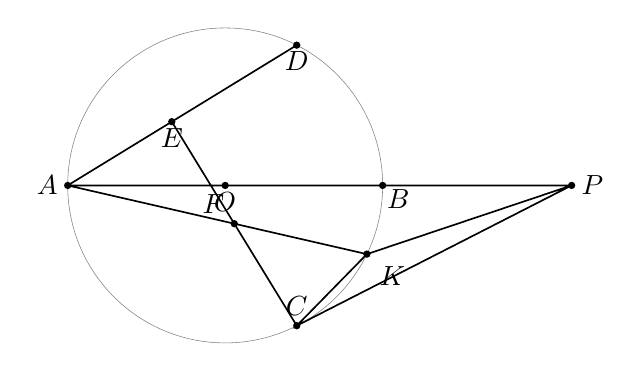
\begin{tikzpicture}[semithick]
\tkzDefPoints{-2/0/A,2/0/B,4.4/0/P}
\tkzDefMidPoint(A,B)\tkzGetPoint{O}
\tkzDrawCircle(O,A)
\tkzTangent[from= P](O,A)\tkzGetPoints{C}{D}
\coordinate(E)at($(A)!(C)!(D)$);
\tkzDefMidPoint(C,E)\tkzGetPoint{F}
\tkzInterLC(A,F)(O,A)\tkzGetPoints{A}{K}

\tkzDrawPoints[size=2,fill=black](A,B,C,D,O,P,F,E,K)
\tkzLabelPoints[left](A)
\tkzLabelPoints[below=-0.4mm](O,D,E)
\tkzLabelPoints[above left](F)
\tkzLabelPoints[above](C)
\tkzLabelPoints[below right=-1mm](B)
\tkzLabelPoints[below right=0.5mm](K)
\tkzLabelPoints[right](P)
\draw(K)--(A)(A)--(P)--(C)--(K)--(P)(C)--(E)(A)--(D);
\end{tikzpicture}
}
\subfloat[]{\label{4.2}
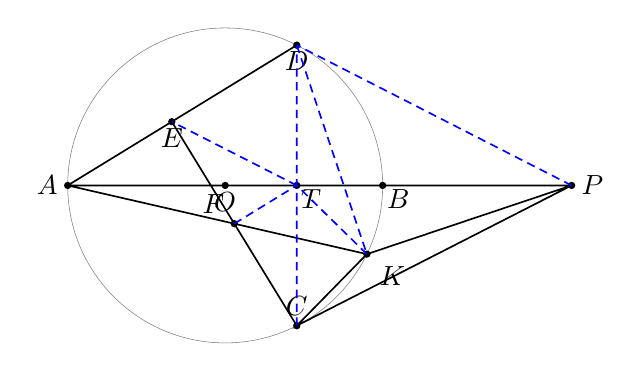
\begin{tikzpicture}[semithick]
\tkzDefPoints{-2/0/A,2/0/B,4.4/0/P}
\tkzDefMidPoint(A,B)\tkzGetPoint{O}
\tkzDrawCircle(O,A)
\tkzTangent[from= P](O,A)\tkzGetPoints{C}{D}
\coordinate(E)at($(A)!(C)!(D)$);
\tkzDefMidPoint(C,E)\tkzGetPoint{F}
\tkzInterLC(A,F)(O,A)\tkzGetPoints{A}{K}
\tkzInterLL(C,D)(A,B)\tkzGetPoint{T}

\tkzDrawPoints[size=2,fill=black](A,B,C,D,O,P,F,E,K,T)
\tkzLabelPoints[left](A)
\tkzLabelPoints[below=-0.4mm](O,D,E)
\tkzLabelPoints[above left](F)
\tkzLabelPoints[above](C)
\tkzLabelPoints[below right=-1mm](B,T)
\tkzLabelPoints[below right=0.5mm](K)
\tkzLabelPoints[right](P)
\draw(K)--(A)(A)--(P)--(C)--(K)--(P)(C)--(E)(A)--(D);
\draw[densely dashed,blue,semithick](P)--(D)(D)--(K)(K)--(T)(T)--(E)(C)--(D)(F)--(T);
\end{tikzpicture}
}
\caption{第 \thefigure 题图}
\end{figure}
\begin{Proof}
如图 \subref{4.2},连接$PD$,根据圆的对称性知,点$D$在$\odot O$上,且$PD$切$\odot O$于$D$.连接$CD$交$AB$于$T$,则$CT\bot AB$,且$T$为$CD$的中点.连接$TE,TK$.

 显然$TF$为$\triangle CDE$的中位线,所以$TF\pxx AD,TF\bot CE$,且$\angle TFK=\angle DAK=\angle TCK$,故$C,F,T,K$四点共圆.于是$\angle KTP=90^\circ-\angle KTC=\angle KCD=\angle KDP$,所以$T,D,P,K$四点共圆,因此$\angle TPK=\angle TDK=\angle PCK$,即$AP$为$\triangle PCK$外接圆的切线.
\end{Proof}
\item 如图 \subref{5.1}, 四边形$ABCD$内接于$\odot O$,且$AC$为$\odot O$的直径. $D$关于$AC$的对称点为$E$, $C$关于$BD$的对称点为$F$. $AF$交$BD$于点$G$, $BE$交$AC$于点$K$.求证: $KG\bot BG$.(2014年新加坡数学奥林匹克公开赛第二轮试题)
\begin{figure}[!ht]
\centering
\subfloat[]{\label{5.1}
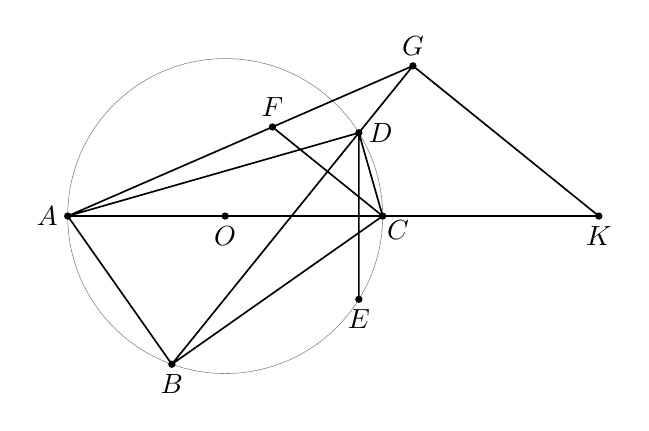
\begin{tikzpicture}[semithick]
\tkzDefPoints{-2/0/A,2/0/C,0.3/0/C1,0.9/0/C2}
\tkzDefMidPoint(A,C)\tkzGetPoint{O}
\tkzDrawCircle(O,C)
\tkzInterCC(A,C1)(O,A)\tkzGetPoints{B1}{B}
\tkzInterCC(C,C2)(O,A)\tkzGetPoints{E}{D}
\tkzInterLL(B,E)(A,C)\tkzGetPoint{K}
\tkzDefPointBy[reflection=over B--D](C)\tkzGetPoint{F}
\tkzInterLL(A,F)(B,D)\tkzGetPoint{G}
\tkzLabelPoints[below right=-1mm](C)
\tkzLabelPoints[below](B,O,E,K)
\tkzLabelPoints[right](D)
\tkzLabelPoints[above](G,F)
\tkzLabelPoints[left](A)
\tkzDrawPoints[size=2,fill=black](D,G,F,E,A,B,O,C,K)
\draw(A)--(G)(G)--(K)(K)--(A)(A)--(B)(B)--(G)(C)--(F)(D)--(E)
(C)--(D)(C)--(B)(A)--(D);
\end{tikzpicture}
}
\subfloat[]{\label{5.2}
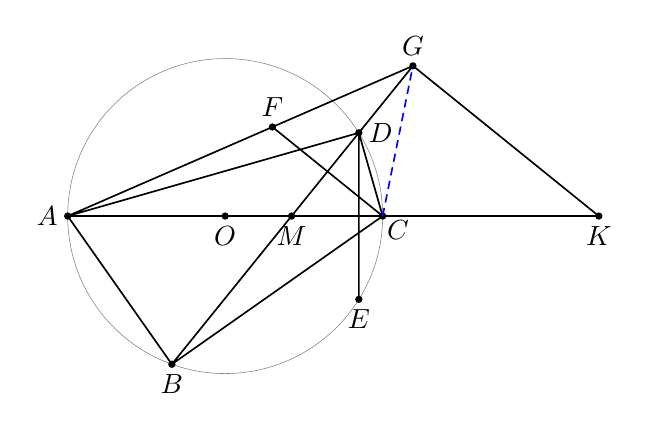
\begin{tikzpicture}[semithick]
\tkzDefPoints{-2/0/A,2/0/C,0.3/0/C1,0.9/0/C2}
\tkzDefMidPoint(A,C)\tkzGetPoint{O}
\tkzDrawCircle(O,C)
\tkzInterCC(A,C1)(O,A)\tkzGetPoints{B1}{B}
\tkzInterCC(C,C2)(O,A)\tkzGetPoints{E}{D}
\tkzInterLL(B,E)(A,C)\tkzGetPoint{K}
\tkzDefPointBy[reflection=over B--D](C)\tkzGetPoint{F}
\tkzInterLL(A,F)(B,D)\tkzGetPoint{G}
\tkzInterLL(B,D)(A,C)\tkzGetPoint{M}
\tkzLabelPoints[below right=-1mm](C)
\tkzLabelPoints[below](B,K,O,E,M)
\tkzLabelPoints[right](D)
\tkzLabelPoints[above](G,F)
\tkzLabelPoints[left](A)
\tkzDrawPoints[size=2,fill=black](D,G,F,E,A,B,O,C,K,M)
\draw(A)--(G)(G)--(K)(K)--(A)(A)--(B)(B)--(G)(C)--(F)(D)--(E)
(C)--(D)(C)--(B)(A)--(D);
\draw[densely dashed,blue,semithick](C)--(G);
\end{tikzpicture}
}
\caption{第 \thefigure 题图}
\end{figure}
\begin{Proof}
{\kaishu 方法一}\quad 如图 \subref{5.2}, 连接$GC$.根据条件,显然点$E$在$\odot O$上,从而$BC$平分$\angle DBE$.设$BD$交$AC$于$M$.注意到$\angle ABC=90^\circ$,所以$AB$为$\angle KBM$的外角平分线,于是知\[\frac{KC}{MC}=\frac{KB}{MB}=\frac{KA}{MA},\]
从而$\frac{AM}{CM}=\frac{AK}{CK}$.

 根据对称性, $GB$平分$\angle AGC$,所以$\frac{AG}{CG}=\frac{AM}{CM}=\frac{AK}{CK}$,所以$KG$为$\angle AGC$的外角 平分线,因此$KG\bot BG$.

{\kaishu 方法二}\quad 如图 \subref{5.2},连接$GC$. 根据条件,显然点$E$在$\odot O$上,从而$BC$平分$\angle DBE$.设$BD$交$AC$于$M$.注意到$\angle ABC=90^\circ$,所以$K,M,C,A$构成一组调和点列.

 根据对称性, $GB$平分$\angle AGC$,根据调和性质知$KG\bot BG$.
\end{Proof}
\item 如图 \subref{6.1}, $PA,PB$分别切$\odot O$于$A,B$, $K$为$\odot O$上一点, $BD\bot OK$于$D$,分别交$KP,KA$于点$E,F$.证明: $E$为$BF$的中点.
\begin{figure}[!ht]\centering
\subfloat[]{\label{6.1}
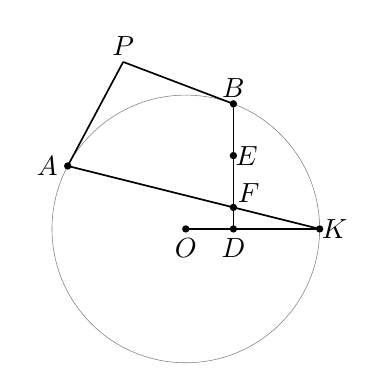
\begin{tikzpicture}[semithick]
\tkzDefPoints{0/0/O,-1.5/0.8/A,0.6/0/A1,1.7/0/K}
\tkzDrawCircle(O,A)
\tkzInterCC(A,A1)(O,A)\tkzGetPoints{B}{B1}
\tkzTangent[at=A](O)\tkzGetPoint{A'}
\tkzTangent[at=B](O)\tkzGetPoint{B'}
\tkzInterLL(A,A')(B,B')\tkzGetPoint{P}
\draw(A)--(P)(P)--(B);
\coordinate(D)at($(O)!(B)!(K)$);
\draw(O)--(K)(B)--(D);
\tkzInterLL(P,K)(B,D)\tkzGetPoint{E}
\tkzInterLL(A,K)(B,D)\tkzGetPoint{F}
\draw(A)--(K);
\tkzLabelPoints[above=-0.5mm](P,B)
\tkzLabelPoints[below](O,D)
\tkzLabelPoints[right=-1mm](E,K)
\tkzLabelPoints[above right=-1mm](F)
\tkzLabelPoints[left](A)
\tkzDrawPoints[size=2,fill=black](O,A,B,D,K,E,F)
\end{tikzpicture}
}\hspace{2cm}
\subfloat[]{\label{6.2}
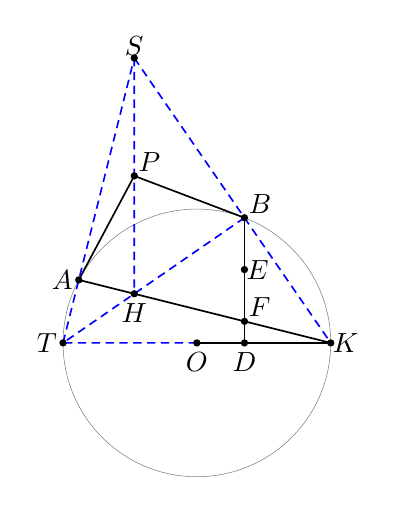
\begin{tikzpicture}[semithick]
\tkzDefPoints{0/0/O,-1.5/0.8/A,0.6/0/A1,1.7/0/K}
\tkzDrawCircle(O,A)
\tkzInterCC(A,A1)(O,A)\tkzGetPoints{B}{B1}
\tkzTangent[at=A](O)\tkzGetPoint{A'}
\tkzTangent[at=B](O)\tkzGetPoint{B'}
\tkzInterLL(A,A')(B,B')\tkzGetPoint{P}
\draw(A)--(P)(P)--(B);
\coordinate(D)at($(O)!(B)!(K)$);
\draw(O)--(K)(B)--(D);
\tkzInterLL(P,K)(B,D)\tkzGetPoint{E}
\tkzInterLL(A,K)(B,D)\tkzGetPoint{F}
\draw(A)--(K);
\tkzInterLC(K,O)(O,K)\tkzGetPoints{K}{T}
\tkzInterLL(T,B)(A,K)\tkzGetPoint{H}
\tkzInterLL(T,A)(K,B)\tkzGetPoint{S}
\draw[densely dashed,blue,semithick](O)--(T)(T)--(S)(S)--(K)
(B)--(T)(S)--(H);
\tkzLabelPoints[below](O,D,H)
\tkzLabelPoints[right=-1mm](E,K)
\tkzLabelPoints[above right=-1mm](F,P,B)
\tkzLabelPoints[above=-1mm](S)
\tkzLabelPoints[left=-0.5mm](A,T)
\tkzDrawPoints[size=2,fill=black](O,A,B,D,K,E,F,T,H,S,P)
\end{tikzpicture}
}
\caption{第 \thefigure 题图}
\end{figure}
\begin{Proof}
如图  \subref{6.2},延长$KO$交$\odot O$于点$T$,延长$TA$交$KB$于点$S$,连接$TB$交$AK$于点$H$.在圆内接六边形$AATBBK$中使用帕斯卡定理,知$S,P,H$三点共线.又$KA\bot TS,TB\bot KS$,故$H$为$\triangle STK$的垂心.进而知$\angle SAP=\angle TKA=\angle ASP$,从而$P$是$SH$的中点.注意到$SH\pxx BD$,所以$E$为$BF$的中点.
\end{Proof}
\item 如图 \subref{7.1}, $\triangle ABC$中, $CA=CB,D$为$AB$的中点, $EF$过点$D$,且使得$\triangle ABC$与$\triangle EFC$有相同的内心.证明: $DE\cdot DF=DA^2$.
\begin{figure}[!ht]\centering
\subfloat[]{\label{7.1}
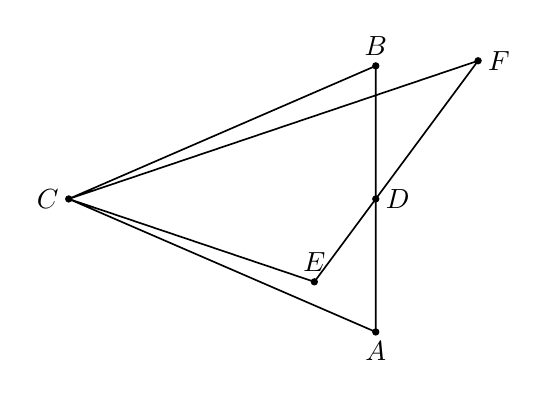
\begin{tikzpicture}[scale=1.3,semithick]
\tkzDefPoints{-3/0/C,0/0/D,0/1.3/B,0/-1.3/A,-0.6/-0.81/E}
\tkzFindAngle(A,C,E)\tkzGetAngle{ACE}
\tkzDefPointBy[rotation=center C angle -\ACE](B)\tkzGetPoint{F1}
\tkzInterLL(C,F1)(E,D)\tkzGetPoint{F}
\draw(C)--(A)(C)--(B)(A)--(B)(C)--(F)(E)--(F)(C)--(E);
\tkzDrawPoints[size=2,fill=black](A,B,C,D,E,F)
\tkzLabelPoints[left](C)
\tkzLabelPoints[above](E,B)
\tkzLabelPoints[below](A)
\tkzLabelPoints[right](D,F)
\end{tikzpicture}
}
\subfloat[]{\label{7.2}
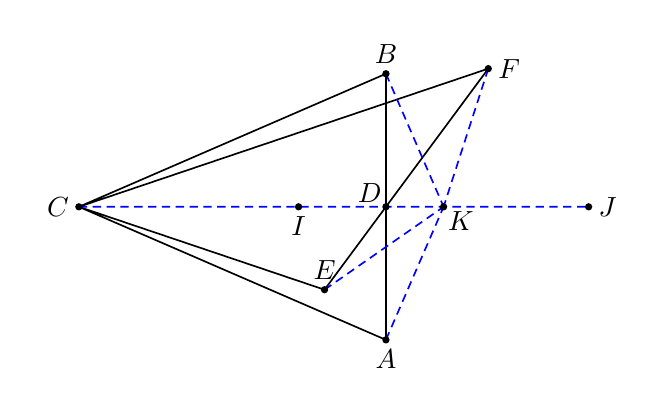
\begin{tikzpicture}[scale=1.3,semithick]
\tkzInit[ymax=1.75,ymin=-1.75,xmin=-3.5,xmax=2.4]
\tkzClip
\tkzDefPoints{-3/0/C,0/0/D,0/1.3/B,0/-1.3/A,-0.6/-0.81/E}
\tkzFindAngle(A,C,E)\tkzGetAngle{ACE}
\tkzDefPointBy[rotation=center C angle -\ACE](B)\tkzGetPoint{F1}
\tkzInterLL(C,F1)(E,D)\tkzGetPoint{F}
\tkzInCenter(C,A,B)\tkzGetPoint{I}
\tkzDefLine[bisector out](C,A,B)\tkzGetPoint{J1}
\tkzInterLL(C,D)(A,J1)\tkzGetPoint{J}
\tkzDefMidPoint(I,J)\tkzGetPoint{K}
\draw(C)--(A)(C)--(B)(A)--(B)(C)--(F)(E)--(F)(C)--(E);
\draw[densely dashed,blue,semithick](C)--(J)(B)--(K)(A)--(K)(F)--(K)(E)--(K);
\tkzLabelPoints[below](I,A)
\tkzLabelPoints[left](C)
\tkzLabelPoints[above](E,B)
\tkzLabelPoints[right](F,J)
\tkzLabelPoints[above left=-1mm](D)
\tkzLabelPoints[below right=-1mm](K)
\tkzDrawPoints[size=2,fill=black](A,B,C,D,E,F,I,J,K)
\end{tikzpicture}
}
\caption{第 \thefigure 题图}
\end{figure}
\begin{Proof}
如图 \subref{7.2},设$\triangle ABC$与$\triangle EFC$共同的内心为$I$,取$\triangle ABC$的$C-$旁心为点$J$,则$C,D,I,J$构成一组调和点列,从而点$J$也为$\triangle CEF$的$C-$旁心.取$IJ$的中点为$K$,则$KI=KJ=KA=KB=KE=KF$,故$A,E,I,B,F<J$六点共圆,所以$DE\cdot DF=DA\cdot DB=DA^2$.
\end{Proof}
\item 如图 \subref{8.1}, $AD$平分$\angle BAC$交$BC$于点$D$, $DE\bot AB$于$E,DF\bot AC$于$F,CE,BF$交于点$K$,证明: $AK\bot BC$.
\begin{figure}[!ht]
\centering
\subfloat[]{\label{8.1}
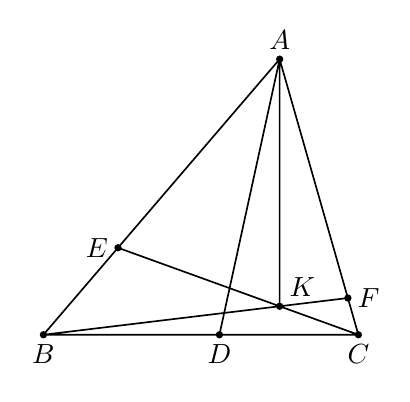
\begin{tikzpicture}[semithick]
\tkzInit[xmax=4.3,xmin=-0.2,ymin=-0.5,ymax=3.9]
\tkzClip
\tkzDefPoints{0/0/B,4/0/C,3/3.5/A}
\tkzDefLine[bisector](B,A,C)\tkzGetPoint{D1}
\tkzInterLL(A,D1)(B,C)\tkzGetPoint{D}
\coordinate(E)at($(A)!(D)!(B)$);
\coordinate(F)at($(A)!(D)!(C)$);
\tkzInterLL(C,E)(B,F)\tkzGetPoint{K}
\draw(A)--(B)(B)--(C)(C)--(A)(B)--(F)(C)--(E)(A)--(D)(A)--(K);
\tkzDrawPoints[size=2,fill=black](A,B,C,D,E,F,K)
\tkzLabelPoints[below](B,C,D)
\tkzLabelPoints[left](E)
\tkzLabelPoints[right](F)
\tkzLabelPoints[above right](K)
\tkzLabelPoints[above](A)
\end{tikzpicture}
}\hspace{2cm}
\subfloat[]{\label{8.2}
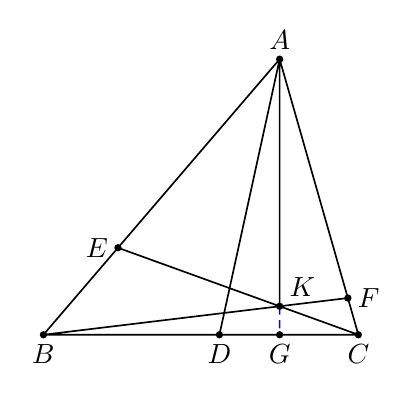
\begin{tikzpicture}[semithick]
\tkzInit[xmax=4.3,xmin=-0.2,ymin=-0.5,ymax=3.9]
\tkzClip
\tkzDefPoints{0/0/B,4/0/C,3/3.5/A}
\tkzDefLine[bisector](B,A,C)\tkzGetPoint{D1}
\tkzInterLL(A,D1)(B,C)\tkzGetPoint{D}
\coordinate(E)at($(A)!(D)!(B)$);
\coordinate(F)at($(A)!(D)!(C)$);
\tkzInterLL(C,E)(B,F)\tkzGetPoint{K}
\draw(A)--(B)(B)--(C)(C)--(A)(B)--(F)(C)--(E)(A)--(D)(A)--(K);
\tkzInterLL(A,K)(B,C)\tkzGetPoint{G}
\draw[densely dashed,blue](K)--(G);
\tkzDrawPoints[size=2,fill=black](A,B,C,D,E,F,K,G)
\tkzLabelPoints[below](B,C,D,G)
\tkzLabelPoints[left](E)
\tkzLabelPoints[right](F)
\tkzLabelPoints[above right](K)
\tkzLabelPoints[above](A)
\end{tikzpicture}
}
\caption{第 \thefigure 题图}
\end{figure}
\begin{Proof}
如图,延长$AH$交$BC$于$G$,根据塞瓦定理得
\[\frac{CG}{BG}\cdot\frac{GE}{EA}\cdot\frac{AF}{FC}=1\Rightarrow
\frac{CG}{BG}=\frac{CF}{BE}=\frac{\tan\angle ABC}{\tan\angle ACB}\Rightarrow AK\bot BC.\]
\end{Proof}
\item 如图 \subref{9.1}, $P$为$\odot O$外一点, $PA,PB$分别切$\odot O$于$A,B$. $C$为$\odot O$上一点,过$C$作$\odot O$的切线分别交$PA,PB$于$E,F$. $OC$交$AB$于$L,LP$交$EF$于$D$.证明: $D$为$EF$的中点.(1991年四川竞赛题)
\begin{figure}[!ht]\centering
\subfloat[]{\label{9.1}
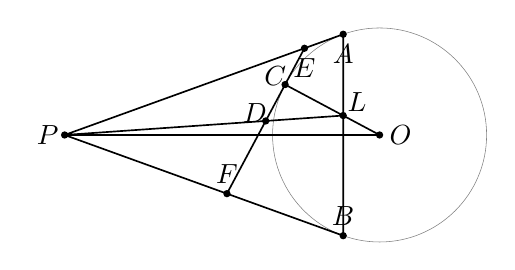
\begin{tikzpicture}[semithick]
\begin{scope}[scale=0.8]
\tkzDefPoints{0/0/O,-5/0/P,-1.5/0.8/C}
\tkzTangent[from =P](O,C)\tkzGetPoints{A}{B}
\tkzDrawCircle(O,C)
\tkzTangent[at=C](O)\tkzGetPoint{C1}
\tkzInterLL(C,C1)(P,A)\tkzGetPoint{E}
\tkzInterLL(C,C1)(P,B)\tkzGetPoint{F}
\tkzInterLL(O,C)(A,B)\tkzGetPoint{L}
\tkzInterLL(P,L)(E,F)\tkzGetPoint{D}
\draw(P)--(O)(A)--(B)(A)--(P)(B)--(P)(E)--(F)
(P)--(L)(O)--(C);
\tkzLabelPoints[right](O)\tkzLabelPoints[above right=-1mm](L)
\tkzLabelPoints[above](B,F)
\tkzLabelPoints[left=-.5mm](P)
\tkzLabelPoints[above left=-2mm](C,D)
\tkzLabelPoints[below](A,E)
\end{scope}
\tkzDrawPoints[size=2,fill=black](O,P,A,B,C,L,E,F,D)
\end{tikzpicture}
}\hspace{1cm}
\subfloat[]{\label{9.2}
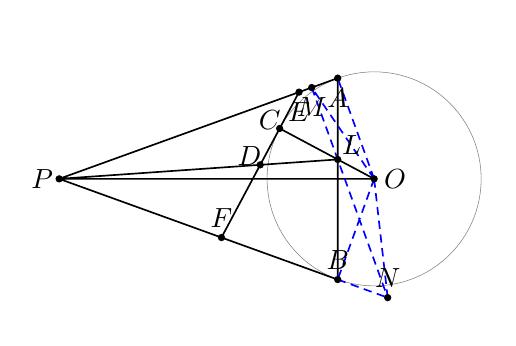
\begin{tikzpicture}[semithick]
\begin{scope}[scale=0.8]
\tkzInit[xmin=-5.5,xmax=1.8,ymin=-2.2,ymax=2.4]
\tkzClip
\tkzDefPoints{0/0/O,-5/0/P,-1.5/0.8/C}
\tkzTangent[from =P](O,C)\tkzGetPoints{A}{B}
\tkzDrawCircle(O,C)
\tkzTangent[at=C](O)\tkzGetPoint{C1}
\tkzInterLL(C,C1)(P,A)\tkzGetPoint{E}
\tkzInterLL(C,C1)(P,B)\tkzGetPoint{F}
\tkzInterLL(O,C)(A,B)\tkzGetPoint{L}
\tkzInterLL(P,L)(E,F)\tkzGetPoint{D}
\draw(P)--(O)(A)--(B)(A)--(P)(B)--(P)(E)--(F)
(P)--(L)(O)--(C);
\tkzDefLine[orthogonal=through L](A,P)\tkzGetPoint{L1}
\tkzInterLL(L,L1)(P,A)\tkzGetPoint{M}
\tkzInterLL(L,L1)(P,B)\tkzGetPoint{N}
\draw[densely dashed,blue](B)--(N)(M)--(N)(N)--(O)(O)--(A)(O)--(M)(O)--(B);
\tkzLabelPoints[right](O)\tkzLabelPoints[above right=-1mm](L)
\tkzLabelPoints[above](B,F,N)
\tkzLabelPoints[left=-.5mm](P)
\tkzLabelPoints[above left=-2mm](C,D)
\tkzLabelPoints[below](A,E,M)
\end{scope}
\tkzDrawPoints[size=2,fill=black](O,P,A,B,C,L,E,F,D,M,N)
\end{tikzpicture}
}
\caption{第 \thefigure 题图}
\end{figure}
\begin{Proof}
如图 \subref{9.2}, 过点$L$作$OC$的垂线分别交$PA,PB$于点$M,N$,注意到$OA\bot PM$, $OB\bot PN$,根据西姆松定理的逆定理知$O,M,P,N$四点共圆.又$OP$平分$\angle APB$,故$OM=ON$,进而知$LM=LN$.而$MN\pxx EF$,故$D$为$EF$的中点.
\end{Proof}
\item 如图 \subref{10.1}, 点$P$为$\odot O$外一点, $PA,PB$分别切$\odot O$于$A,B$. $C$为$\odot O$上一点, $CD\bot AB$于$D$,过$C$作$\odot O$的切线分别交$PA,PB$于$E,F$,证明: $CD$平分$\angle EDF$.
\begin{figure}[!ht]
\centering
\subfloat[]{\label{10.1}
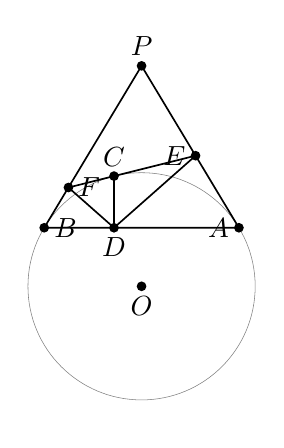
\begin{tikzpicture}[scale=0.7,semithick]
\tkzDefPoints{0/0/O,-0.5/2/C,0/4/P}
\draw(0,-2.4);
\tkzTangent[from=P](O,C)\tkzGetPoints{A}{B}
\coordinate(D)at($(A)!(C)!(B)$);
\tkzDrawCircle(O,C)
\tkzTangent[at=C](O)\tkzGetPoint{C1}
\tkzInterLL(C,C1)(P,A)\tkzGetPoint{E}
\tkzInterLL(C,C1)(P,B)\tkzGetPoint{F}
\draw(P)--(A)(A)--(B)(P)--(B)(E)--(F)(E)--(D)(D)--(F)(C)--(D);
\tkzDrawPoints[size=2.86,fill=black](P,O,C,A,B,D,E,F)
\tkzLabelPoints[above](P,C)
\tkzLabelPoints[right](B,F)
\tkzLabelPoints[left](A,E)
\tkzLabelPoints[below](D,O)
\end{tikzpicture}
}
\subfloat[]{\label{10.2}
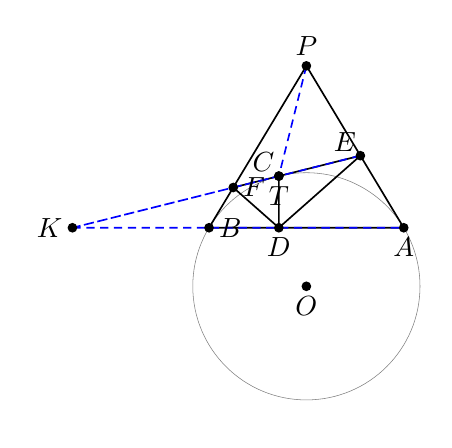
\begin{tikzpicture}[scale=0.7,semithick]
\tkzDefPoints{0/0/O,-0.5/2/C,0/4/P}
\draw(0,-2.4);
\tkzTangent[from=P](O,C)\tkzGetPoints{A}{B}
\coordinate(D)at($(A)!(C)!(B)$);
\tkzDrawCircle(O,C)
\tkzTangent[at=C](O)\tkzGetPoint{C1}
\tkzInterLL(C,C1)(P,A)\tkzGetPoint{E}
\tkzInterLL(C,C1)(P,B)\tkzGetPoint{F}
\draw(P)--(A)(A)--(B)(P)--(B)(E)--(F)(E)--(D)(D)--(F)(C)--(D);
\tkzInterLL(E,F)(B,A)\tkzGetPoint{K}
\tkzInterLC(P,C)(O,C)\tkzGetPoints{T}{C1}
\draw[densely dashed,blue](P)--(T)(E)--(K)(K)--(A)(K)--(T);
\tkzLabelPoints[above](P)
\tkzLabelPoints[right](B,F)
\tkzLabelPoints[left](K)\tkzLabelPoints[above left=-1mm](C,E)
\tkzLabelPoints[below](D,A,O,T)
\tkzDrawPoints[size=2.86,fill=black](P,O,C,A,B,D,E,F,T,K)
\end{tikzpicture}
}
\subfloat[]{\label{10.3}
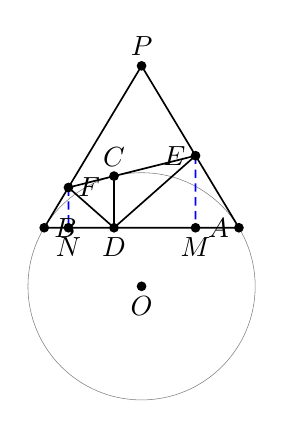
\begin{tikzpicture}[scale=0.7,semithick]
\tkzDefPoints{0/0/O,-0.5/2/C,0/4/P}
\draw(0,-2.4);
\tkzTangent[from=P](O,C)\tkzGetPoints{A}{B}
\coordinate(D)at($(A)!(C)!(B)$);
\tkzDrawCircle(O,C)
\tkzTangent[at=C](O)\tkzGetPoint{C1}
\tkzInterLL(C,C1)(P,A)\tkzGetPoint{E}
\tkzInterLL(C,C1)(P,B)\tkzGetPoint{F}
\draw(P)--(A)(A)--(B)(P)--(B)(E)--(F)(E)--(D)(D)--(F)(C)--(D);
\coordinate(M)at($(A)!(E)!(B)$);\coordinate(N)at($(A)!(F)!(B)$);
\draw[densely dashed,blue](E)--(M)(F)--(N);
\tkzLabelPoints[above](P,C)
\tkzLabelPoints[right](B,F)
\tkzLabelPoints[left](E,A)
\tkzLabelPoints[below](D,O,M,N)
\tkzDrawPoints[size=2.86,fill=black](P,O,C,A,B,D,E,F,M,N)
\end{tikzpicture}
}
\caption{第 \thefigure 题图}
\end{figure}
\begin{Proof}
{\kaishu 方法一}\quad 如图 \subref{10.2},延长$FE$交$BA$于点$K$,过$K$作$\odot O$的切线$KT$切$\odot O$于点$T$,注意到点$K$在$P$关于$\odot O$的极线上,过点$P$也在点$K$关于$\odot O$的极线上,从而知$P,C,T$共线,所以$K,C,E,F$构成一组调和点列.而$CD\bot AB$,故$CD$平分$\angle EDF$.

{\kaishu 方法二}\quad 如图 \subref{10.3},作$EM\bot AB$于$M$,作$FN\bot AB$于$N$,则
\[\frac{EM}{FN}=\frac{FA}{FB}=\frac{EC}{FC}=\frac{MD}{ND},\]
故$\triangle EMD\xs\triangle FND$,所以$\angle EDM=\angle FDN$,因此$\angle EDC=\angle FDC$.
\end{Proof}
\item 如图 \subref{11.1}, $AB$为$\odot O$的直径, $PA$切$\odot O$于点$A$, $PCD$为$\odot O$的一条割线, $PO$交$BD$于$E$.证明: $AC\bot AE$.
\begin{figure}[!ht]\centering
\subfloat[]{\label{11.1}
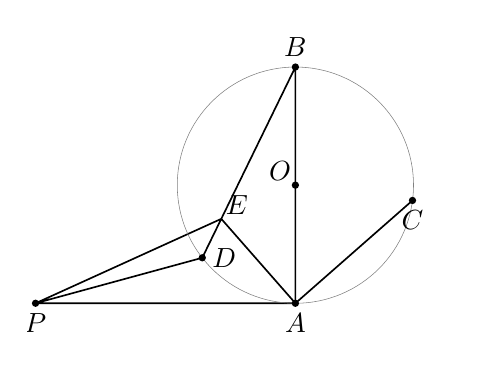
\begin{tikzpicture}[semithick]
\tkzInit[xmin=-3.4,xmax=2,ymin=-0.5,ymax=3.5]
\tkzClip
\tkzDefPoints{0/0/A,0/3/B,-3.3/0/P,0/0.9/Q}
\tkzDefMidPoint(A,B)\tkzGetPoint{O}
\tkzInterLC(P,Q)(O,A)\tkzGetPoints{D}{C}
\tkzInterLL(P,O)(B,D)\tkzGetPoint{E}
\draw(P)--(A)(A)--(B)(P)--(D)(P)--(E)(A)--(E)(A)--(C)(B)--(D);
\tkzDrawCircle(O,A)
\tkzDrawPoints[size=2,fill=black](O,A,B,C,D,P)
\tkzLabelPoints[below](A,P,C)
\tkzLabelPoints[above](B)
\tkzLabelPoints[above left=-1mm](O)
\tkzLabelPoints[right](D)
\tkzLabelPoints[above right=-1mm](E)
\end{tikzpicture}
}\hspace{2cm}
\subfloat[]{\label{11.2}
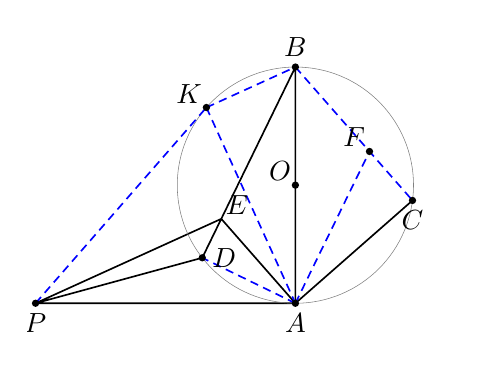
\begin{tikzpicture}[semithick]
\tkzInit[xmin=-3.4,xmax=2,ymin=-0.5,ymax=3.5]
\tkzClip
\tkzDefPoints{0/0/A,0/3/B,-3.3/0/P,0/0.9/Q}
\tkzDefMidPoint(A,B)\tkzGetPoint{O}
\tkzInterLC(P,Q)(O,A)\tkzGetPoints{D}{C}
\tkzInterLL(P,O)(B,D)\tkzGetPoint{E}
\draw(P)--(A)(A)--(B)(P)--(D)(P)--(E)(A)--(E)(A)--(C)(B)--(D);
\tkzDrawCircle(O,A)
\tkzDefPointBy[reflection=over P--O](A)\tkzGetPoint{K}
\tkzInterLL(B,C)(P,E)\tkzGetPoint{F}
\draw[densely dashed,blue](P)--(K)(K)--(B)(K)--(A)(B)--(C)(A)--(F)(A)--(D);
\tkzDrawPoints[size=2,fill=black](O,A,B,C,D,P,K,F)
\tkzLabelPoints[below](A,P,C)
\tkzLabelPoints[above](B)
\tkzLabelPoints[above left=-1mm](O,K,F)
\tkzLabelPoints[right](D)
\tkzLabelPoints[above right=-1mm](E)
\end{tikzpicture}
}

\subfloat[]{\label{11.3}
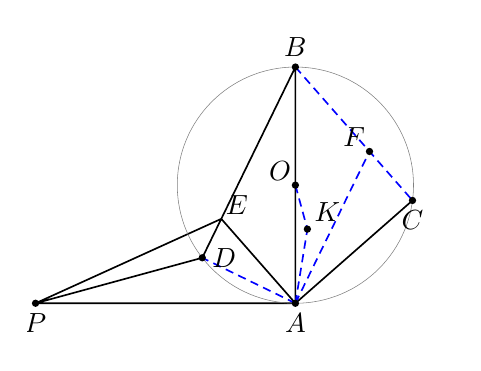
\begin{tikzpicture}[semithick]
\tkzInit[xmin=-3.4,xmax=2,ymin=-0.5,ymax=3.5]
\tkzClip
\tkzDefPoints{0/0/A,0/3/B,-3.3/0/P,0/0.9/Q}
\tkzDefMidPoint(A,B)\tkzGetPoint{O}
\tkzInterLC(P,Q)(O,A)\tkzGetPoints{D}{C}
\tkzInterLL(P,O)(B,D)\tkzGetPoint{E}
\draw(P)--(A)(A)--(B)(P)--(D)(P)--(E)(A)--(E)(A)--(C)(B)--(D);
\tkzDrawCircle(O,A)
\coordinate(K)at($(C)!(O)!(D)$);
\tkzInterLL(B,C)(P,E)\tkzGetPoint{F}
\draw[densely dashed,blue](B)--(C)(A)--(F)(A)--(K)(O)--(K)(A)--(D);
\tkzDrawPoints[size=2,fill=black](O,A,B,C,D,P,K,F)
\tkzLabelPoints[below](A,P,C)
\tkzLabelPoints[above](B)
\tkzLabelPoints[above left=-1mm](O,F)
\tkzLabelPoints[right](D)
\tkzLabelPoints[above right=-1mm](E)
\tkzLabelPoints[above right=-0.5mm](K)
\end{tikzpicture}
}\hspace{2cm}
\subfloat[]{\label{11.4}
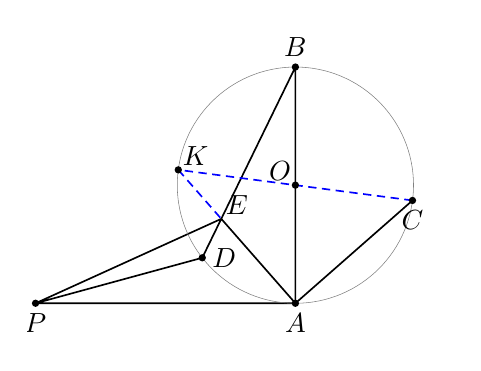
\begin{tikzpicture}[semithick]
\tkzInit[xmin=-3.4,xmax=2,ymin=-0.5,ymax=3.5]
\tkzClip
\tkzDefPoints{0/0/A,0/3/B,-3.3/0/P,0/0.9/Q}
\tkzDefMidPoint(A,B)\tkzGetPoint{O}
\tkzInterLC(P,Q)(O,A)\tkzGetPoints{D}{C}
\tkzInterLL(P,O)(B,D)\tkzGetPoint{E}
\draw(P)--(A)(A)--(B)(P)--(D)(P)--(E)(A)--(E)(A)--(C)(B)--(D);
\tkzDrawCircle(O,A)
\tkzDefPointBy[rotation=center O angle 180](C)\tkzGetPoint{K}
\draw[densely dashed,blue](C)--(K)(K)--(E);
\tkzDrawPoints[size=2,fill=black](O,A,B,C,D,P,K)
\tkzLabelPoints[below](A,P,C)
\tkzLabelPoints[above](B)
\tkzLabelPoints[above left=-1mm](O)
\tkzLabelPoints[right](D)
\tkzLabelPoints[above right=-1mm](E,K)
\end{tikzpicture}
}
\caption{第 \thefigure 题图}
\end{figure}
\begin{Proof}
{\kaishu 方法一}\quad 如图 \subref{11.2}, 作$PK$且$\odot O$于$K$,则$PE\bot AK,BK\bot AK$,所以$KB\pxx PE$.又注意到四边形$CADK$为调和四边形,故$BK,BA,BC,BD$构成一组调和线束,从而$O$为$EF$的中点.进而知四边形$AEBF$为平行四边形,于是$AE\pxx BC,AE\bot AC$.

{\kaishu 方法二}\quad 如图 \subref{11.3},连接$BC$交$PE$于$F$,作$OK\bot CD$于$K$,则$K$为$CD$的中点.注意到$O,K,A,P$四点共圆,故$\angle AKD=\angle FOB$.又$\angle ADK=\angle FBO$,则$\triangle ADK\xs\triangle FBO$.注意到$O$为$AB$的中点,故$\triangle ADC\xs\triangle FBA$,从而知$\angle FAB=\angle ACD=\angle ABD$,故$AF\pxx BD$,于是四边形$AEBF$为平行四边形,所以$AE\pxx BC,AE\bot AC$.

{\kaishu 方法三}\quad 如图 \subref{11.4},延长$AE$交$\odot O$于点$K$,在圆内接六边形$AABDCK$中使用帕斯卡定理,注意到$P,O,E$共线,故$C,O,K$共线,所以$AE\bot AC$.
\end{Proof}
\item 如图 \subref{12.1}, $AB$为半圆$O$的直径, $C,D$为半圆上两点.过$B$作半圆的切线交$CD$于$P$,直线$PO$分别交直线$CA,AD$于点$E,F$.求证: $OE=OF$.(2007年第四届东南地区数学奥林匹克试题)
\begin{figure}[!ht]\centering
\subfloat[]{\label{12.1}
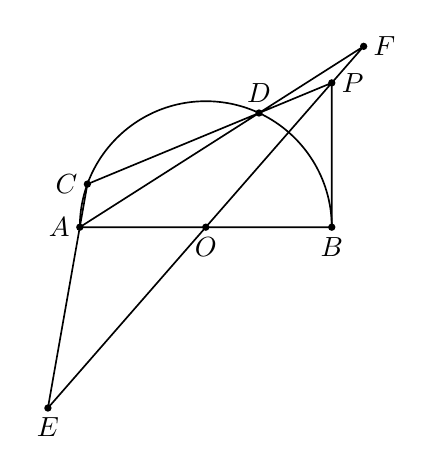
\begin{tikzpicture}[semithick]
\begin{scope}[scale=0.8]
\tkzDefPoints{-2/0/A,2/0/B,0/0/O,2/2/Q}
\coordinate(C)at(160:2);\coordinate(D)at(65:2);
\tkzInterLL(B,Q)(C,D)\tkzGetPoint{P}
\tkzInterLL(P,O)(C,A)\tkzGetPoint{E}
\tkzInterLL(P,O)(A,D)\tkzGetPoint{F}
\draw(B)arc(0:180:2);
\draw(A)--(B)(C)--(E)(E)--(F)(A)--(F)(C)--(P)(P)--(B);
\tkzLabelPoints[left](A,C)
\tkzLabelPoints[above](D)
\tkzLabelPoints[right](P,F)
\tkzLabelPoints[below](O,B,E)
\end{scope}
\tkzDrawPoints[size=2,fill=black](O,A,C,B,D,E,F,P)
\end{tikzpicture}
}
\subfloat[]{\label{12.2}
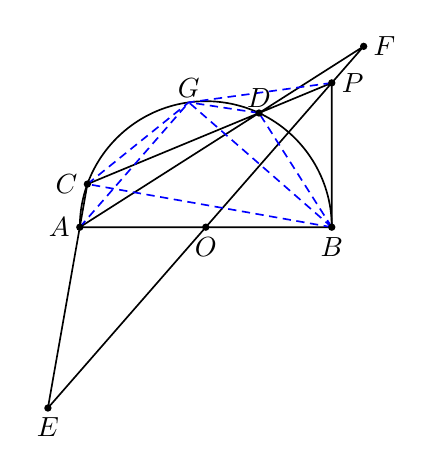
\begin{tikzpicture}[semithick]
\begin{scope}[scale=0.8]
\tkzDefPoints{-2/0/A,2/0/B,0/0/O,2/2/Q}
\coordinate(C)at(160:2);\coordinate(D)at(65:2);
\tkzInterLL(B,Q)(C,D)\tkzGetPoint{P}
\tkzInterLL(P,O)(C,A)\tkzGetPoint{E}
\tkzInterLL(P,O)(A,D)\tkzGetPoint{F}
\draw(B)arc(0:180:2);
\draw(A)--(B)(C)--(E)(E)--(F)(A)--(F)(C)--(P)(P)--(B);
\tkzDefPointBy[reflection=over O--P](B)\tkzGetPoint{G}
\draw[densely dashed,blue](A)--(G)(B)--(G)(B)--(D)(B)--(C)(C)--(G)
(P)--(G)(D)--(G);
\tkzLabelPoints[left](A,C)
\tkzLabelPoints[above=-0.6mm](D,G)
\tkzLabelPoints[right](P,F)
\tkzLabelPoints[below](O,B,E)
\end{scope}
\tkzDrawPoints[size=2,fill=black](O,A,C,B,D,E,F,P)
\end{tikzpicture}
}
\subfloat[]{\label{12.3}
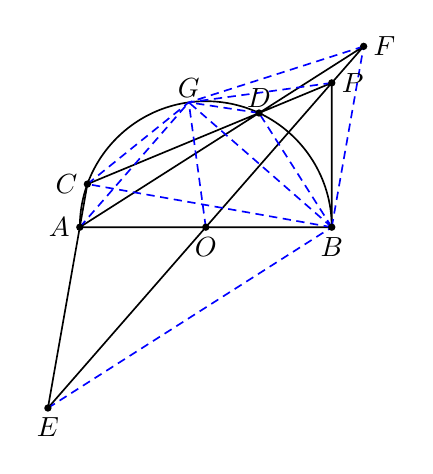
\begin{tikzpicture}[semithick]
\begin{scope}[scale=0.8]
\tkzDefPoints{-2/0/A,2/0/B,0/0/O,2/2/Q}
\coordinate(C)at(160:2);\coordinate(D)at(65:2);
\tkzInterLL(B,Q)(C,D)\tkzGetPoint{P}
\tkzInterLL(P,O)(C,A)\tkzGetPoint{E}
\tkzInterLL(P,O)(A,D)\tkzGetPoint{F}
\draw(B)arc(0:180:2);
\draw(A)--(B)(C)--(E)(E)--(F)(A)--(F)(C)--(P)(P)--(B);
\tkzDefPointBy[reflection=over O--P](B)\tkzGetPoint{G}
\draw[densely dashed,blue](A)--(G)(B)--(G)(B)--(D)(B)--(C)(C)--(G)
(P)--(G)(D)--(G)(O)--(G)(E)--(B)(B)--(F)(F)--(G);
\tkzLabelPoints[left](A,C)
\tkzLabelPoints[above=-0.6mm](D,G)
\tkzLabelPoints[right](P,F)
\tkzLabelPoints[below](O,B,E)
\end{scope}
\tkzDrawPoints[size=2,fill=black](O,A,C,B,D,E,F,P)
\end{tikzpicture}
}
\caption{第 \thefigure 题图}
\end{figure}
\begin{Proof}
{\kaishu 方法一}\quad 如图 \subref{12.2}, 过$P$作$PG$切半圆$O$于$G$,连接$GA,GB,GC,GD,BC,BD$.易知$OP\bot BG,AG\bot BG$,所以$AG\pxx OP$.又四边形$CBDG$为调和四边形,所以$AC,AD,AG,AB$构成一组调和线束.又因为$AG\pxx OP$,所以$OE=OF$.

{\kaishu 方法二}\quad 如图 \subref{12.3}, 作$PG$切半圆$O$于$G$,则$B,G$关于$P,O$对称,且$P,B,O,G$四点共圆.所以$\angle GPO=\angle GBA=\angle GDA$,于是知$D,P,F,G$四点共圆.进而知$\angle FBP=\angle FGP=\angle FDP=\angle CDA=\angle CBA$,故$\angle FBC=\angle PBA=90^\circ=\angle ECB$,所以$FB\pxx EA$.而$O$为$AB$的中点,所以$O$为$EF$的中点.
\end{Proof}
\item 如图 \subref{13.1}, $\triangle ABC$中, $D,E$分别为$AB,AC$上一点,且$DE\pxx BC,BE,CD$交于点$F$. $\triangle BDF$的外接圆$\odot O$与$\triangle CEF$的外接圆$\odot P$交于点$G$,求证: $\angle BAF=\angle CAG$.
\begin{figure}[!ht]\centering
\subfloat[]{\label{13.1}
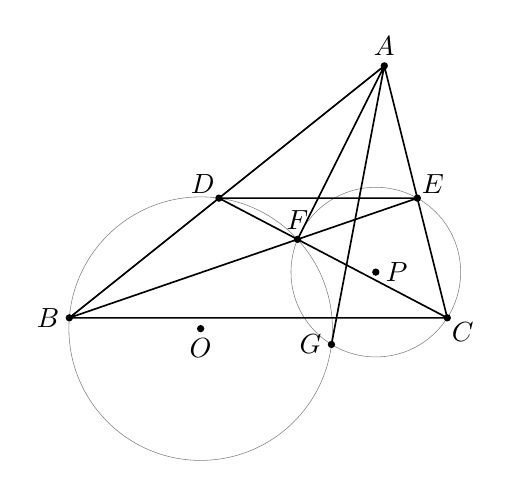
\begin{tikzpicture}[semithick]
\begin{scope}[scale=0.8]
\tkzDefPoints{-3/0/B,3/0/C,2/4/A,0/1.9/K}
\tkzDefLine[parallel=through K](B,C)\tkzGetPoint{L}
\tkzInterLL(K,L)(A,B)\tkzGetPoint{D}
\tkzInterLL(K,L)(A,C)\tkzGetPoint{E}
\tkzInterLL(B,E)(C,D)\tkzGetPoint{F}
\tkzCircumCenter(B,D,F)\tkzGetPoint{O}
\tkzCircumCenter(C,E,F)\tkzGetPoint{P}
\tkzInterCC(O,B)(P,C)\tkzGetPoints{F}{G}
\tkzDrawCircle(O,B)\tkzDrawCircle(P,C)
\draw(A)--(B)(B)--(C)(C)--(A)(D)--(E)(C)--(D)(B)--(E)
(A)--(F)(A)--(G);
\tkzLabelPoints[below](O)
\tkzLabelPoints[left](G,B)
\tkzLabelPoints[below right=-1mm](C)
\tkzLabelPoints[above right=-1mm](E)
\tkzLabelPoints[above left=-1mm](D)
\tkzLabelPoints[above](F,A)
\tkzLabelPoints[right](P)
\end{scope}
\tkzDrawPoints[size=2,fill=black](O,A,B,C,D,E,F,G,P)
\end{tikzpicture}
}
\subfloat[]{\label{13.2}
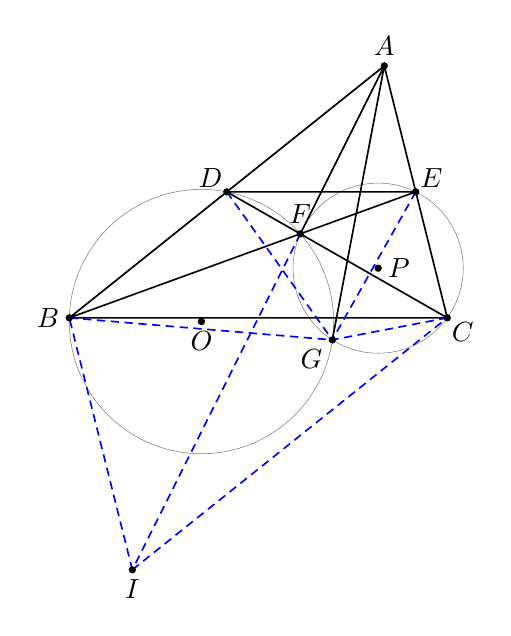
\begin{tikzpicture}[semithick]
\begin{scope}[scale=0.8]
\tkzDefPoints{-3/0/B,3/0/C,2/4/A,0/2/K}
\tkzDefLine[parallel=through K](B,C)\tkzGetPoint{L}
\tkzInterLL(K,L)(A,B)\tkzGetPoint{D}
\tkzInterLL(K,L)(A,C)\tkzGetPoint{E}
\tkzInterLL(B,E)(C,D)\tkzGetPoint{F}
\tkzCircumCenter(B,D,F)\tkzGetPoint{O}
\tkzCircumCenter(C,E,F)\tkzGetPoint{P}
\tkzInterCC(O,B)(P,C)\tkzGetPoints{F}{G}
\tkzDrawCircle(O,B)\tkzDrawCircle(P,C)
\draw(A)--(B)(B)--(C)(C)--(A)(D)--(E)(C)--(D)(B)--(E)
(A)--(F)(A)--(G);
\tkzInterLL(A,F)(B,C)\tkzGetPoint{H}
\tkzCalcLength[cm](A,H)\tkzGetLength(AH)
\tkzDefLine[parallel=through H](A,H)\tkzGetPoint{I}
\draw[densely dashed,blue](F)--(I)(D)--(G)(E)--(G)(B)--(G)(C)--(G)
(I)--(B)(I)--(C);
\tkzLabelPoints[below](O,I)
\tkzLabelPoints[left](B)\tkzLabelPoints[below left](G)
\tkzLabelPoints[below right=-1mm](C)
\tkzLabelPoints[above right=-1mm](E)
\tkzLabelPoints[above left=-1mm](D)
\tkzLabelPoints[above](F,A)
\tkzLabelPoints[right](P)
\end{scope}
\tkzDrawPoints[size=2,fill=black](O,A,B,C,D,E,F,G,P,I)
\end{tikzpicture}
}

\caption{第 \thefigure 题图}
\end{figure}
\begin{Proof}
如图 \subref{13.2},延长$AF$交$BC$于$H$.因为$DE\pxx BC$,所以$H$为$BC$的中点,延长$AH$到$I$,使得$AH=HI$,连接$BC,CI$,则四边形$ABIC$是平行四边形.

 连接$GC,GE,GD,GB,FG$,因为$\angle ACG=\angle BFG=\angle BDG$,所以$A,D,G,C$四点共圆.于是知$\angle DGC=180^\circ-\angle BAC=\angle ABI$.同理可知$A,B,G,E$四点共圆,所以$\angle DBG=\angle CEG,\angle BDG=\angle ECG$,所以$\triangle BDG\xs \triangle ECG$,所以
\[\frac{DG}{CG}=\frac{BD}{CE}=\frac{AB}{AC}=\frac{AB}{IB},\]
所以$\triangle DGC\xs\triangle ABI$,因此$\angle BAF=\angle GDC=\angle CAG$.
\end{Proof}
\begin{note}
点$G$即为完全四边形$ADFEBC$的\emph{密克点}.
\end{note}
\item 如图 \subref{14.1}, $\odot O,\odot P$交于$A,B$两点, $BO,PA$的延长线交于点$C,CD,CE$分别切$\odot O,\odot P$于$D,E$,连接$DE$交$AB$于$F$.求证: $F$为$DE$的中点.(深圳黎誉俊老师题)
\begin{figure}[!ht]\centering
\subfloat[]{\label{14.1}
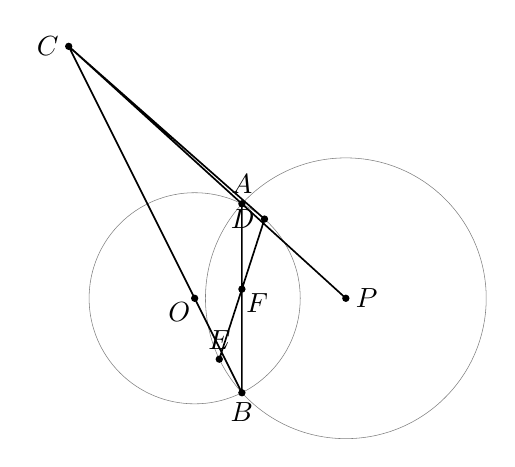
\begin{tikzpicture}[scale=1.2,semithick]
\tkzDefPoints{0/0/O,0.5/1/A,0.5/-1/B,1.6/0/P}
\tkzDrawCircle(O,A)\tkzDrawCircle(P,A)
\tkzInterLL(P,A)(B,O)\tkzGetPoint{C}
\tkzTangent[from=C](O,A)\tkzGetPoints{D}{D1}
\tkzTangent[from=C](P,A)\tkzGetPoints{E1}{E}
\tkzInterLL(D,E)(A,B)\tkzGetPoint{F}
\draw(C)--(D)(D)--(E)(C)--(P)(C)--(B)(B)--(A);
\tkzLabelPoints[left](C,D)
\tkzLabelPoints[below left=-1mm](O)
\tkzLabelPoints[above](A,E)
\tkzLabelPoints[below](B)
\tkzLabelPoints[below right=-1mm](F)
\tkzLabelPoints[right](P)
\tkzDrawPoints[size=2,fill=black](O,A,B,P,C,D,E,F)
\end{tikzpicture}
}\hspace{1cm}
\subfloat[]{\label{14.2}
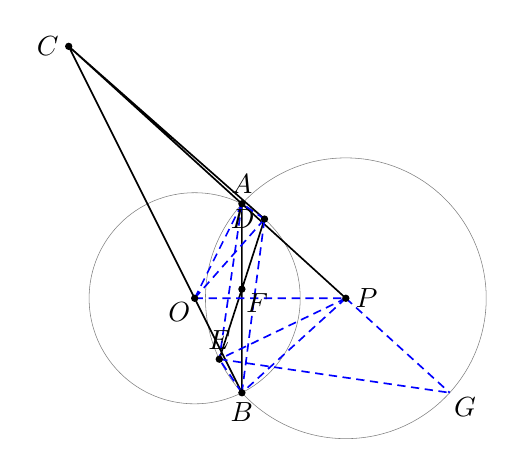
\begin{tikzpicture}[scale=1.2,semithick]
\tkzDefPoints{0/0/O,0.5/1/A,0.5/-1/B,1.6/0/P}
\tkzDrawCircle(O,A)\tkzDrawCircle(P,A)
\tkzInterLL(P,A)(B,O)\tkzGetPoint{C}
\tkzTangent[from=C](O,A)\tkzGetPoints{D}{D1}
\tkzTangent[from=C](P,A)\tkzGetPoints{E1}{E}
\tkzInterLL(D,E)(A,B)\tkzGetPoint{F}
\tkzInterLC(A,P)(P,A)\tkzGetPoints{G1}{G}

\draw(C)--(D)(D)--(E)(C)--(P)(C)--(B)(B)--(A);
\draw[densely dashed,blue](D)--(A)(B)--(D)(O)--(A)(O)--(D)(O)--(P)
(B)--(E)(P)--(B)(P)--(E)(P)--(G)(E)--(G)(A)--(E);
\tkzLabelPoints[left](C,D)
\tkzLabelPoints[above](A,E)
\tkzLabelPoints[below left=-1mm](O)
\tkzLabelPoints[below](B)
\tkzLabelPoints[below right=-1mm](F,G)
\tkzLabelPoints[right](P)
\tkzDrawPoints[size=2,fill=black](O,A,B,P,C,D,E,F)
\end{tikzpicture}
}
\caption{第 \thefigure 题图}
\end{figure}
\begin{Proof}
如图 \subref{14.2}, 延长$AP$交$\odot P$于$G$,连接$EG,EP,EA,EB,OP,oA,OD,AD,BD$.设$\odot O,\odot P$的半径分别为$r_1,r_2$.因为
\[\frac{CO}{CP}=\frac{\sin\angle CPO}{\sin\angle BOP}=\frac{\sin\angle APO}{\angle AOP}=\frac{AO}{AP}=\frac{r_1}{r_2},\]
所以$\triangle CDO\xs \triangle CEP$,于是知$\frac{CD}{CE}=\frac{r_1}{r_2}$.进而可知$\triangle CDB\xs\triangle CEG\xs\triangle CAE$,于是$\frac{DB}{AE}=\frac{CD}{CA}=\frac{CB}{CE}$.由$\frac{CD}{CA}=\frac{CB}{CE}$知$\triangle CDA\xs\triangle CBE$,从而$\frac{DA}{BE}=\frac{CA}{CE}$,因此
\begin{align*}
\frac{S_{\triangle DAB}}{S_{\triangle EAB}}&=\frac{DA\cdot DB\sin\angle ADB}{EA\cdot EB\sin\angle AEB}=\frac{DA}{BE}\cdot\frac{DB}{AE}\cdot\frac{\sin\angle ADB}{\sin\angle AEB}\\
&=\frac{CD}{CA}\cdot\frac{CA}{CE}\cdot\frac{\sin\angle AOP}{\sin\angle APO}
=\frac{CD}{CE}\cdot\frac{\sin\angle AOP}{\sin\angle APO}=\frac{r_1}{r_2}\cdot\frac{r_2}{r_1}=1.
\end{align*}
所以$F$为$DE$的中点.
\end{Proof}
\item 如图 \subref{15.1}, 半径不相等的两圆$\odot O,\odot P$交于$A,B$两点,过点$A$的直线$CD$分别交$\odot O,\odot P$于$C,D$. $CB$延长线交$\odot P$于$F$, $DB$交$\odot O$于$E$.过$A$作$CD$的垂线交$EF$的中垂线于$G$,求证: $AG^2=EG^2+AC\cdot AD$.(2013年CMO第一题推广)
\begin{figure}[!ht]\centering
\subfloat[]{\label{15.1}
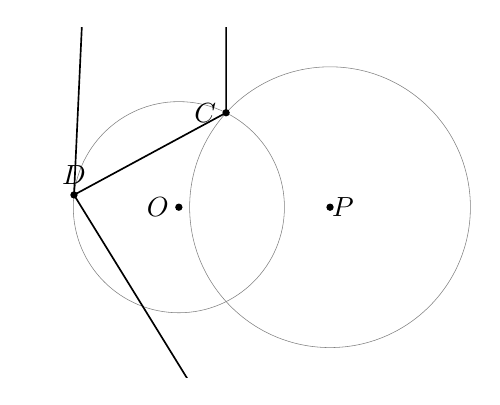
\begin{tikzpicture}[scale=1.2,semithick]
\tkzInit[ymax=1.9,ymin=-1.8,xmin=-1.6,xmax=3.1]
\tkzClip
\tkzDefPoints{0/0/O,0.5/1/A,0.5/-1/B,1.6/0/P,0/0.73/K}
\tkzDrawCircle(O,A)\tkzDrawCircle(P,A)
\tkzInterLC(A,K)(O,A)\tkzGetPoints{C}{A}
\tkzInterLC(A,C)(P,A)\tkzGetPoints{A}{D}
\tkzInterLC(C,B)(P,A)\tkzGetPoints{F}{B}
\tkzInterLC(D,B)(O,A)\tkzGetPoints{E}{B}
\tkzDefLine[mediator](E,F)\tkzGetPoints{E1}{F1}
\tkzDefLine[orthogonal=through A](C,D)
\tkzGetPoint{G1}
\tkzInterLL(A,G1)(E1,F1)\tkzGetPoint{G}

\draw(C)--(D)(C)--(F)(B)--(D)(A)--(G)(G)--(E)(G)--(D)
(A)--(E)(A)--(F)(E)--(F);
\tkzLabelPoints[left](C,O)
\tkzLabelPoints[above](A,D)
\tkzLabelPoints[right=-1mm](E,P)
\tkzLabelPoints[below](G,B,F)
\tkzDrawPoints[size=2,fill=black](O,A,B,P,C,D,F,E,G)
\end{tikzpicture}
}\hspace{2cm}
\subfloat[]{\label{15.2}
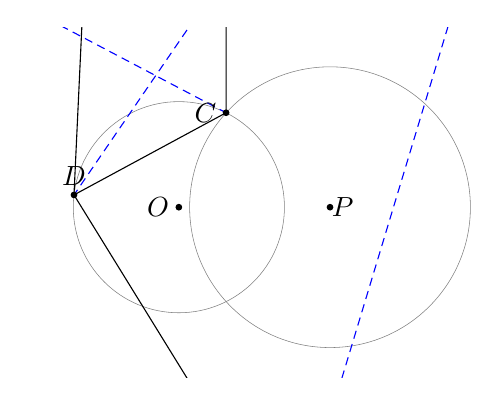
\begin{tikzpicture}[scale=1.2]
\tkzInit[ymax=1.9,ymin=-1.8,xmin=-1.6,xmax=3.1]
\tkzClip
\tkzDefPoints{0/0/O,0.5/1/A,0.5/-1/B,1.6/0/P,0/0.73/K}
\tkzDrawCircle(O,A)\tkzDrawCircle(P,A)
\tkzInterLC(A,K)(O,A)\tkzGetPoints{C}{A}
\tkzInterLC(A,C)(P,A)\tkzGetPoints{A}{D}
\tkzInterLC(C,B)(P,A)\tkzGetPoints{F}{B}
\tkzInterLC(D,B)(O,A)\tkzGetPoints{E}{B}
\tkzDefLine[mediator](E,F)\tkzGetPoints{E1}{F1}
\tkzDefLine[orthogonal=through A](C,D)
\tkzGetPoint{G1}
\tkzInterLL(A,G1)(E1,F1)\tkzGetPoint{G}

\draw(C)--(D)(C)--(F)(B)--(D)(A)--(G)(G)--(E)(G)--(D)
(A)--(E)(A)--(F)(E)--(F);
\draw[densely dashed,blue](E)--(C)(A)--(B)(G)--(F)(F)--(D);
\tkzLabelPoints[left](C,O)
\tkzLabelPoints[above](A,D)
\tkzLabelPoints[right=-1mm](E,P)
\tkzLabelPoints[below](G,B,F)
\tkzDrawPoints[size=2,fill=black](O,A,B,P,C,D,F,E,G)
\end{tikzpicture}
}
\caption{第 \thefigure 题图}
\end{figure}
\begin{Proof}
如图 \subref{15.2}, 连接$AB,CE,DF,GF$.因为
\[\angle CAE=\angle CBE=\angle FBD=\angle FAD,\angle ACE=\angle ABD=\angle AFD,\]
所以$\triangle ACE\xs\triangle AFD$,因此$AC\cdot AD=AE\cdot AF$.又由于$\odot O,\odot P$的半径不相等,所以$AE\ne AF$.又$GE=GF$,
\[\angle EAG=90^\circ-\angle CAE=90^\circ-\angle CBE=90^\circ-\angle FBD=90^\circ-\angle FAD=\angle FAG,\]
所以$A,E,G,F$四点共圆.易知$\triangle GEK\xs\triangle GAE$,所以$EG^2=GK\cdot AG$.又易知$\triangle AEK\xs\triangle AGF$,所以$AK\cdot AG=AE\cdot AF=AC\cdot AD$,因此
\[EG^2+AC\cdot AD=GK\cdot AG+AK\cdot AG=AG^2.\]
\end{Proof}
\item 如图 \subref{16.1}, $\triangle ABC$内接于$\odot O,D$为$BC$的中点, $AD$交$\odot O$于$E$.过点$E$作$EF\pxx BC$,交$\odot O$于$F$,过点$C$作$CG\bot AC$,交$AE$于$G$.求证: $\angle AGC=\angle FGC$.
\begin{figure}[!ht]
\centering
\subfloat[]{\label{16.1}
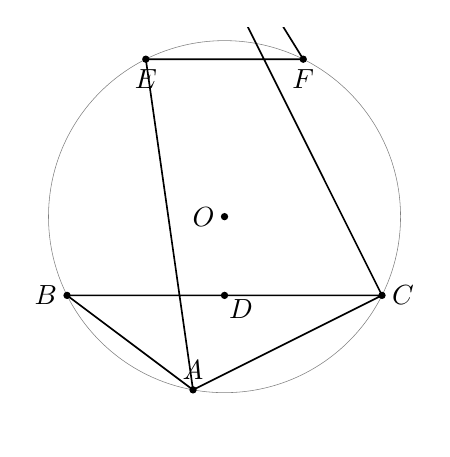
\begin{tikzpicture}[semithick]
\tkzInit[xmin=-2.5,xmax=2.5,ymin=-1.7,ymax=3.4]
\tkzClip
\tkzDefPoints{-2/0/B,2/0/C,1/3/A}
\tkzCircumCenter(A,B,C)\tkzGetPoint{O}
\tkzDefMidPoint(B,C)\tkzGetPoint{D}
\tkzInterLC(A,D)(O,A)\tkzGetPoints{A}{E}
\tkzDrawCircle(O,A)
\tkzDefLine[parallel=through E](B,C)
\tkzGetPoint{F}
\tkzInterLC(E,F)(O,A)\tkzGetPoints{F}{E}
\tkzDefLine[orthogonal=through C](A,C)
\tkzGetPoint{G}
\tkzInterLL(C,G)(A,E)\tkzGetPoint{G}
\draw(A)--(B)(B)--(C)(C)--(A)(C)--(G)(E)--(F)(F)--(G)(A)--(E);
\tkzLabelPoints[left](O,B,G)
\tkzLabelPoints[below](E,F)
\tkzLabelPoints[right](C)
\tkzLabelPoints[above](A)
\tkzLabelPoints[below right=-1mm](D)
\tkzDrawPoints[size=2,fill=black](O,A,B,C,D,E,F,G)
\end{tikzpicture}
}\hspace{1.5cm}
\subfloat[]{\label{16.2}
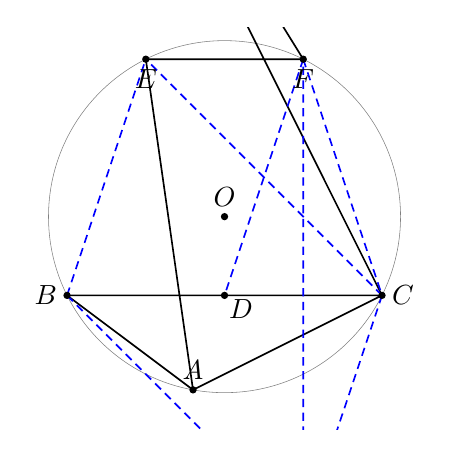
\begin{tikzpicture}[semithick]
\tkzInit[xmin=-2.5,xmax=2.5,ymin=-1.7,ymax=3.4]
\tkzClip
\tkzDefPoints{-2/0/B,2/0/C,1/3/A}
\tkzCircumCenter(A,B,C)\tkzGetPoint{O}
\tkzDefMidPoint(B,C)\tkzGetPoint{D}
\tkzInterLC(A,D)(O,A)\tkzGetPoints{A}{E}
\tkzDrawCircle(O,A)
\tkzDefLine[parallel=through E](B,C)
\tkzGetPoint{F}
\tkzInterLC(E,F)(O,A)\tkzGetPoints{F}{E}
\tkzDefLine[orthogonal=through C](A,C)
\tkzGetPoint{G}
\tkzInterLL(C,G)(A,E)\tkzGetPoint{G}
\draw(A)--(B)(B)--(C)(C)--(A)(C)--(G)(E)--(F)(F)--(G)(A)--(E);
\tkzDefLine[parallel=through C](E,B)\tkzGetPoint{K}
\draw[densely dashed,blue](C)--(K)(B)--(K)(B)--(E)(C)--(E)
(K)--(F)(F)--(C)(B)--(E)(C)--(E)(F)--(D);
\tkzLabelPoints[left](B,G)
\tkzLabelPoints[below](E,F)
\tkzLabelPoints[right](C,K)
\tkzLabelPoints[above](A,O)
\tkzLabelPoints[below right=-1mm](D)
\tkzDrawPoints[size=2,fill=black](O,A,B,C,D,E,F,G,K)
\end{tikzpicture}
}
\caption{第 \thefigure 题图}
\end{figure}
\begin{Proof}
如图 \subref{16.2}, 连接$BE,CF$,过点$C$作$CK\pxx BE$交$AE$于$K$.因为$BD=CD$,所以四边形$BECK$为平行四边形.于是知
\[CK=BE=CF,\angle KCD=\angle EBC=\angle FCB,\]
所以$\triangle KCD\qd \triangle FCD$,所以$KF\bot BC$.于是知
\[\angle CFK=90^\circ-\angle FCD=90^\circ-\angle EBC=90^\circ-\angle EAC=\angle CGK,\]
所以$G,F,C,K$四点共圆.而$CK=CF$,所以$\angle AGC=\angle FGC$.
\end{Proof}
\item 如图 \subref{17.1}, $\triangle ABC$的内切圆$\odot I$切$BC$于$D$,过$I$作$IE\pxx AD$交$BC$于$E$,过$E$作$\odot I$的切线,分别交$AB,AC$与$F,G$.求证: $E$为$FG$的中点.
\begin{figure}[!ht]
\centering
\subfloat[]{\label{17.1}
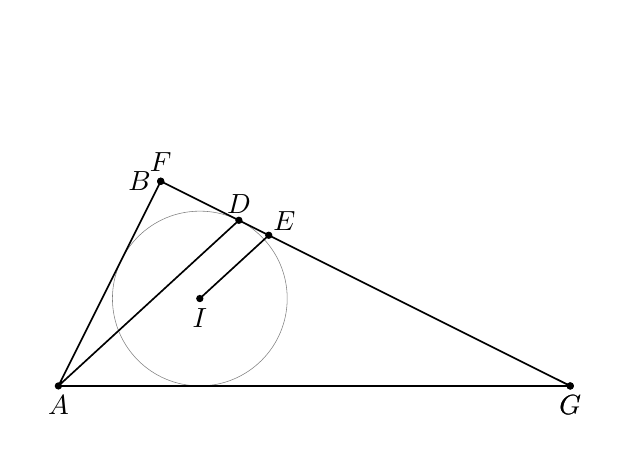
\begin{tikzpicture}[scale=1.3,semithick]
\tkzInit[xmin=-0.3,xmax=5.3,ymin=-0.6,ymax=3.5]
\tkzClip
\tkzDefPoints{0/0/A,5/0/C,1/2/B}
\tkzInCenter(A,B,C)\tkzGetPoint{I}
\coordinate(D)at($(B)!(I)!(C)$);
\tkzDrawCircle(I,D)
\tkzDefLine[parallel=through I](A,D)
\tkzGetPoint{E}
\tkzInterLL(I,E)(B,C)\tkzGetPoint{E}
\tkzTangent[from=E](I,D)\tkzGetPoints{E1}{H}
\tkzInterLL(E,H)(A,B)\tkzGetPoint{F}
\tkzInterLL(E,H)(A,C)\tkzGetPoint{G}
\draw(A)--(F)(B)--(C)(A)--(C)(F)--(G)(A)--(D)(I)--(E);
\tkzLabelPoints[below](A,I,C,G)
\tkzLabelPoints[above right=-1mm](E)
\tkzLabelPoints[above](F)
\tkzLabelPoints[left](B)
\tkzLabelPoints[above=-0.4mm](D)
\tkzDrawPoints[size=2,fill=black](A,C,B,D,E,I,F,G)
\end{tikzpicture}
}
\subfloat[]{\label{17.2}
\begin{tikzpicture}[scale=1.3,semithick]
\tkzInit[xmin=-0.3,xmax=5.3,ymin=-0.6,ymax=3.5]
\tkzClip
\tkzDefPoints{0/0/A,5/0/C,1/2/B}
\tkzInCenter(A,B,C)\tkzGetPoint{I}
\coordinate(D)at($(B)!(I)!(C)$);
\tkzDrawCircle(I,D)
\tkzDefLine[parallel=through I](A,D)
\tkzGetPoint{E}
\tkzInterLL(I,E)(B,C)\tkzGetPoint{E}
\tkzTangent[from=E](I,D)\tkzGetPoints{E1}{H}
\tkzInterLL(E,H)(A,B)\tkzGetPoint{F}
\tkzInterLL(E,H)(A,C)\tkzGetPoint{G}
\draw(A)--(F)(B)--(C)(A)--(C)(F)--(G)(A)--(D)(I)--(E);
\tkzInterLL(D,H)(E,I)\tkzGetPoint{M}
\tkzInterLL(M,I)(A,H)\tkzGetPoint{N}
\draw[densely dashed,blue](A)--(H)(I)--(N)(D)--(H);
\tkzLabelPoints[below](A,C,G,N)
\tkzLabelPoints[above right=-1mm](E)
\tkzLabelPoints[above=-0.5mm](I,F)
\tkzLabelPoints[left=-0.3mm](M,B)
\tkzLabelPoints[above=-0.4mm](D)
\tkzDrawPoints[size=2,fill=black](A,C,B,D,E,I,F,G,H,M,N)
\end{tikzpicture}
}
\caption{第 \thefigure 题图}
\end{figure}
\begin{Proof}
如图 \subref{17.2}, 设$\odot I$切$FG$于点$H$,连接$DH$交$IE$于$M$,则$M$为$DH$的中点.连接$AH$,延长$MI$交$AH$于$N$,因为$MN\pxx AD$,所以$N$为$AH$的中点.在退化的圆外切四边形$EFAG$中使用牛顿定理,即知$E$为$FG$的中点.
\end{Proof}
\item 如图 \subref{18.1}, $\odot P,\odot Q$交于$A,B$两点,它们的外公切线$CD$分别切$\odot P,\odot Q$于$C,D$. $E$为$BA$延长线上一点, $EC$交$\odot P$于$F,ED$交$\odot Q$于$G,AH$平分$\angle FAG$交$FG$于$H$.求证: $\angle FCH=\angle GDH$.(深圳黎誉俊老师题)
\begin{figure}[!ht]
\centering
\subfloat[]{\label{18.1}
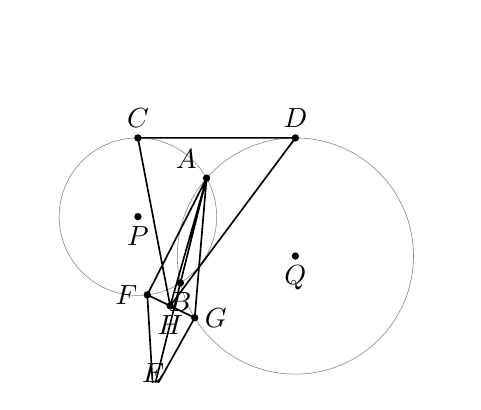
\begin{tikzpicture}[semithick]
\tkzInit[xmin=-1.4,xmax=4,ymin=-3.1,ymax=1.4]
\tkzClip
\tkzDefPoints{0/0/C,2/0/D,0/-1/P,2/-1.5/Q}
\tkzDrawCircle(P,C)\tkzDrawCircle(Q,D)
\tkzInterCC(P,C)(Q,D)\tkzGetPoints{A}{B}
\tkzInterLC(B,A)(P,D)\tkzGetPoints{E}{E1}
\tkzInterLC(E,C)(P,A)\tkzGetPoints{F}{C}
\tkzInterLC(E,D)(Q,A)\tkzGetPoints{D}{G}
\tkzDefLine[bisector](F,A,G)\tkzGetPoint{H}
\tkzInterLL(A,H)(F,G)\tkzGetPoint{H}
\draw(E)--(F)(E)--(G)(F)--(G)(C)--(D)(A)--(F)(A)--(G)(A)--(H)(A)--(B)
(E)--(A)(C)--(H)(D)--(H);
\tkzLabelPoints[left](F)
\tkzLabelPoints[above](E,C,D)
\tkzLabelPoints[below](P,Q,B)
\tkzLabelPoints[above left](A)
\tkzLabelPoints[below](H)
\tkzLabelPoints[right](G)
\tkzDrawPoints[size=2,fill=black](P,Q,C,D,A,B,E,F,G,H)
\end{tikzpicture}
}
\subfloat[]{\label{18.2}
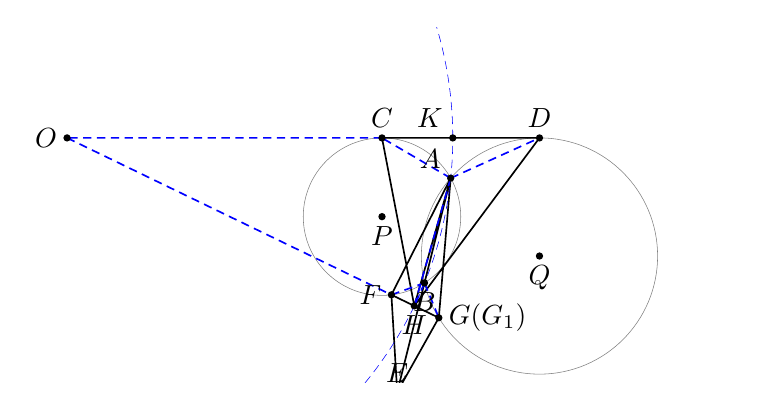
\begin{tikzpicture}[semithick]
\tkzInit[xmin=-4.5,xmax=4.75,ymin=-3.1,ymax=1.4]
\tkzClip
\tkzDefPoints{0/0/C,2/0/D,0/-1/P,2/-1.5/Q}
\tkzDrawCircle(P,C)\tkzDrawCircle(Q,D)
\tkzInterCC(P,C)(Q,D)\tkzGetPoints{A}{B}
\tkzInterLC(B,A)(P,D)\tkzGetPoints{E}{E1}
\tkzInterLC(E,C)(P,A)\tkzGetPoints{F}{C}
\tkzInterLC(E,D)(Q,A)\tkzGetPoints{D}{G}
\tkzDefLine[bisector](F,A,G)\tkzGetPoint{H}
\tkzInterLL(A,H)(F,G)\tkzGetPoint{H}
\draw(E)--(F)(E)--(G)(F)--(G)(C)--(D)(A)--(F)(A)--(G)(A)--(H)(A)--(B)
(E)--(A)(C)--(H)(D)--(H);
\tkzInterLL(P,Q)(D,C)\tkzGetPoint{O}
\tkzInterLC(C,D)(O,A)\tkzGetSecondPoint{K}
\tkzDrawCircle[densely dashed,draw=blue](O,A)
\draw[densely dashed,blue](C)--(O)(O)--(F)(F)--(B)(B)--(G)
(A)--(C)(A)--(D)(A)--(H)(B)--(H);

\tkzLabelPoints[left](O,F)
\tkzLabelPoints[above](E,C,D)
\tkzLabelPoints[below](P,Q,B)
\tkzLabelPoints[above left](A,K)
\tkzLabelPoints[below](H)
\node[right]at(G){$G(G_1)$};
\tkzDrawPoints[size=2,fill=black](P,Q,C,D,A,B,E,F,G,H,O,K)
\end{tikzpicture}
}
\caption{第 \thefigure 题图}
\end{figure}
\begin{Proof}
因为$E$在$\odot O,\odot P$的根轴上,所以$F,C,D,G$四点共圆.

如图 \subref{18.2},设点$O$为$\odot P,\odot Q$的外位似中心,则$\odot P,\odot Q$以点$O$为反演中心互为反形.延长$OF$交$\odot Q$于$G_1$,则$OA^2=OC\cdot OD=OF\cdot OG$,所以$F,C,D,G_1$四点共圆,于是点$G_1$与点$G$重合为一点.以$O$为圆心,以$OA$为半径作$\odot O$交$CD$于$K$,则$\odot O$为$K$关于$C,D$的阿波罗尼斯圆.由于$AH$平分$\angle FAG$,所以点$H$为$\odot O$与$FG$的交点,从而$\odot O$也为点$H$关于$F,G$的阿波罗尼斯圆.于是
\begin{align*}
\angle FCH-\angle GDH&=(\angle FCA-\angle HCA)-(\angle GDA-\angle HDA)\\
&=(\angle FCA-\angle GDA)-(\angle HCA-\angle HDA)\\
&=[(180^\circ-\angle FBA)-(180^\circ-\angle GBA)]\\
&\quad -[(\angle HCA-\angle HKA)-(\angle HDA+\angle HKA)+2\angle HKA]\\
&=(\angle GBA-\angle FBA)\\
&\quad-[(\angle KAC-\angle KHC)-(\angle KAD-\angle KHD)+2\angle HKA]\\
&=[(\angle GBH+\angle HBA)-(\angle FBH-\angle HBA)-2\angle HKA]\\
&=2\angle HBA-2\angle HKA=0,
\end{align*}
所以$\angle FCH=\angle GDH$.
\end{Proof}
\item 如图 \subref{19.1}, $\odot O$为$\triangle ABC$的外接圆, $I,E$分别为$\triangle ABD$的内心和一个旁心. $\angle BAC$的外角平分线交$BC$的延长线于$D$. $IF\bot DE$于$F$,交$\odot O$于$G$,求证: $G$为$IF$的中点.(潘成华老师题)
\begin{figure}[!ht]
\centering
\subfloat[]{\label{19.1}
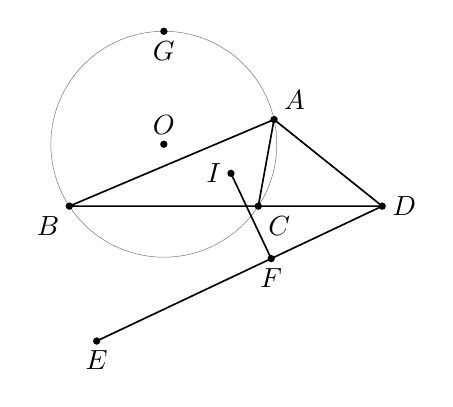
\begin{tikzpicture}[semithick]
\tkzDefPoints{-1.2/-0.4/B,1.2/-0.4/C,1.4/0.7/A}
\tkzCircumCenter(A,B,C)\tkzGetPoint{O}
\tkzInCenter(A,B,C)\tkzGetPoint{I}
\tkzDefLine[orthogonal=through B](B,I)\tkzGetPoint{B1}
\tkzInterLL(B,B1)(A,I)\tkzGetPoint{E}
\tkzDrawCircle(O,A)
\tkzDefLine[orthogonal=through A](A,I)\tkzGetPoint{A1}
\tkzInterLL(A,A1)(B,C)\tkzGetPoint{D}
\coordinate(F)at($(E)!(I)!(D)$);
\tkzInterLC(I,F)(O,A)\tkzGetPoints{G1}{G}
\draw(A)--(B)(B)--(D)(C)--(A)(I)--(F)(E)--(D)(A)--(D);
\tkzLabelPoints[above](O)
\tkzLabelPoints[above right](A)
\tkzLabelPoints[below right](C)
\tkzLabelPoints[below left](B)
\tkzLabelPoints[below](E,F,G)
\tkzLabelPoints[right](D)
\tkzLabelPoints[left](I)
\tkzDrawPoints[size=2,fill=black](A,B,C,O,E,I,D,F,G)
\end{tikzpicture}
}
\subfloat[]{\label{19.2}
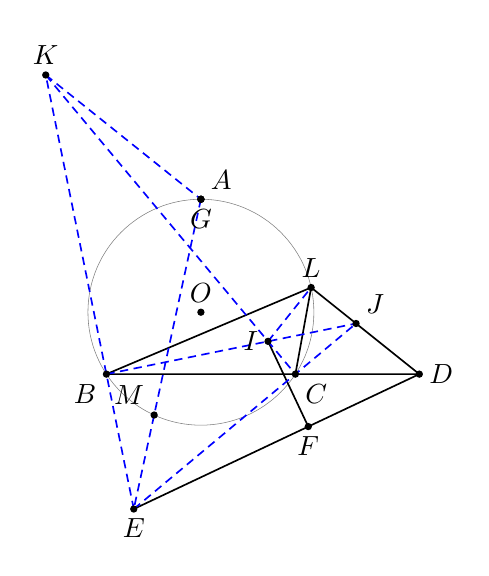
\begin{tikzpicture}[semithick]
\tkzInit[xmin=-2.2,xmax=3.3,ymin=-2.6,ymax=4]
\tkzClip
\tkzDefPoints{-1.2/-0.4/B,1.2/-0.4/C,1.4/0.7/A}
\tkzCircumCenter(A,B,C)\tkzGetPoint{O}
\tkzInCenter(A,B,C)\tkzGetPoint{I}
\tkzDefLine[orthogonal=through B](B,I)\tkzGetPoint{B1}
\tkzInterLL(B,B1)(A,I)\tkzGetPoint{E}
\tkzDrawCircle(O,A)
\tkzDefLine[orthogonal=through A](A,I)\tkzGetPoint{A1}
\tkzInterLL(A,A1)(B,C)\tkzGetPoint{D}
\coordinate(F)at($(E)!(I)!(D)$);
\tkzInterLC(I,F)(O,A)\tkzGetPoints{G1}{G}
\draw(A)--(B)(B)--(D)(C)--(A)(I)--(F)(E)--(D)(A)--(D);
\tkzInterLL(E,B)(A,D)\tkzGetPoint{K}
\tkzInterLL(E,C)(A,D)\tkzGetPoint{J}
\tkzInterLC(K,J)(O,A)\tkzGetPoints{L}{A}
\tkzInterLC(A,E)(O,A)\tkzGetPoints{A}{M}
\draw[densely dashed,blue](E)--(K)(K)--(A)(E)--(J)(A)--(E)
(B)--(J)(K)--(C)(I)--(L);
\tkzLabelPoints[above left](M)
\tkzLabelPoints[above](O,L,K)
\tkzLabelPoints[above right](A,J)
\tkzLabelPoints[below right](C)
\tkzLabelPoints[below left](B)
\tkzLabelPoints[below](E,F,G)
\tkzLabelPoints[right](D)
\tkzLabelPoints[left](I)
\tkzDrawPoints[size=2,fill=black](A,B,C,O,E,I,D,F,G,J,K,L,M,G)
\end{tikzpicture}
}
\subfloat[]{\label{19.3}
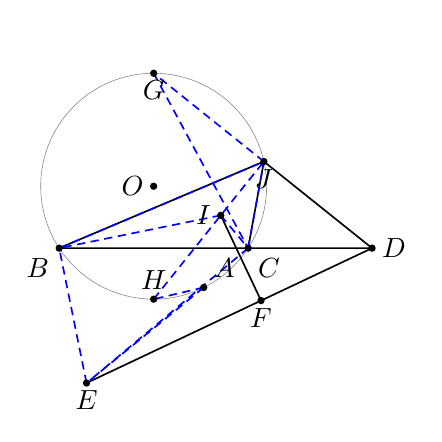
\begin{tikzpicture}[semithick]
\tkzInit[xmin=-1.6,xmax=3.3,ymin=-2.5,ymax=2.4]
\tkzClip
\tkzDefPoints{-1.2/-0.4/B,1.2/-0.4/C,1.4/0.7/A}
\tkzCircumCenter(A,B,C)\tkzGetPoint{O}
\tkzInCenter(A,B,C)\tkzGetPoint{I}
\tkzDefLine[orthogonal=through B](B,I)\tkzGetPoint{B1}
\tkzInterLL(B,B1)(A,I)\tkzGetPoint{E}
\tkzDrawCircle(O,A)
\tkzDefLine[orthogonal=through A](A,I)\tkzGetPoint{A1}
\tkzInterLL(A,A1)(B,C)\tkzGetPoint{D}
\coordinate(F)at($(E)!(I)!(D)$);
\tkzInterLC(I,F)(O,A)\tkzGetPoints{G1}{G}
\draw(A)--(B)(B)--(D)(C)--(A)(I)--(F)(E)--(D)(A)--(D);
\tkzInterLC(A,E)(O,A)\tkzGetPoints{A}{J}
\tkzInterLC(D,A)(O,A)\tkzGetPoints{H}{A}
\draw[densely dashed,blue](A)--(E)(E)--(B)(I)--(B)(I)--(C)(H)--(J)
(B)--(J)(C)--(J)(G)--(C)(J)--(G)(A)--(H)(H)--(I)(C)--(E);
\tkzLabelPoints[above](H)
\tkzLabelPoints[above right](A)
\tkzLabelPoints[below right](C)
\tkzLabelPoints[below left](B)
\tkzLabelPoints[below=-0.3mm](E,F,G,J)
\tkzLabelPoints[right](D)
\tkzLabelPoints[left](I,O)
\tkzDrawPoints[size=2,fill=black](A,B,C,O,E,I,D,F,G,J,H)
\end{tikzpicture}
}
\caption{第 \thefigure 题图}
\end{figure}
\begin{Proof}
{\kaishu 方法一}\quad 如图 \subref{19.2}, 连接$EB,EC$并延长,分别交直线$AC$于$K,J$.易知$K,J$也是$\triangle ABC$的旁心,且$\triangle ABC$为$\triangle EKJ$的垂足三角形, $I$为$\triangle EKJ$的垂心,从而$\odot O$为$\triangle EKJ$的九点圆.

 设$\odot O$分别交$KJ,IE$于$L,M$,则知$L,M$分别为$KJ$和$IE$的中点.又易知$K,B,C,J$四点共圆,且圆心为$L$,于是知$LI\bot DE$,所以$L,I,G,F$四点共线.因此$\angle MGL=\angle MAL=90^\circ$,从而$MG\pxx DE$.又$M$为$IE$的中点,所以$G$为$IF$的中点.

{\kaishu 方法二}\quad 如图 \subref{19.3},连接$AE$交$\odot O$于$J$,则知$A,I,J,E$共线,且$J$为$IE$的中点.又因为$\angle IBE=\angle ICE=\angle IFE$,所以$B,E,F,C,I$五点共圆,且圆心为$J$.

 延长$DA$交$\odot O$于$H$,则知$DF\cdot DE=DC\cdot DB=DA\cdot DH$,所以$H,A,E,F$四点共圆,于是知$\angle HFE=\angle HAE=90^\circ$,所以$H,I,G,F$四点共线.又$\angle HGJ=\angle HAJ=90^\circ$,所以$JG\pxx EF$,故$G$为$IF$的中点.
\end{Proof}
\item 如图 \subref{20.1},在锐角$\triangle ABC$中, $\angle B>\angle C,F$是$BC$的中点, $BE,CD$是高, $G,H$分别是$FD,FE$的中点.若过$A$且平行于$BC$的直线交$GH$于$I$,求证: $AI=FI$.
\begin{figure}[!ht]
\centering
\subfloat[]{\label{20.1}
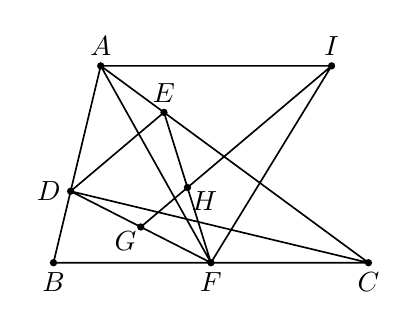
\begin{tikzpicture}[semithick]
\tkzDefPoints{0/0/B,4/0/C,0.6/2.5/A,2/2.5/I}
\tkzDefMidPoint(B,C)\tkzGetPoint{F}
\coordinate(D)at($(A)!(C)!(B)$);
\coordinate(E)at($(A)!(B)!(C)$);
\tkzDefMidPoint(F,D)\tkzGetPoint{G}
\tkzDefMidPoint(F,E)\tkzGetPoint{H}
\tkzInterLL(A,I)(G,H)\tkzGetPoint{I}
\draw(A)--(I)(A)--(B)(B)--(C)(C)--(A)(D)--(E)(D)--(C)
(E)--(F)(D)--(F)(G)--(I)(A)--(F)(I)--(F);
\tkzLabelPoints[below](B,F,C)
\tkzLabelPoints[above](A,I,E)
\tkzLabelPoints[left](D)
\tkzLabelPoints[below left=-1mm](G)
\tkzLabelPoints[below right=-1mm](H)
\tkzDrawPoints[size=2,fill=black](A,B,C,D,E,F,G,H,I)
\end{tikzpicture}
}
\subfloat[]{\label{20.2}
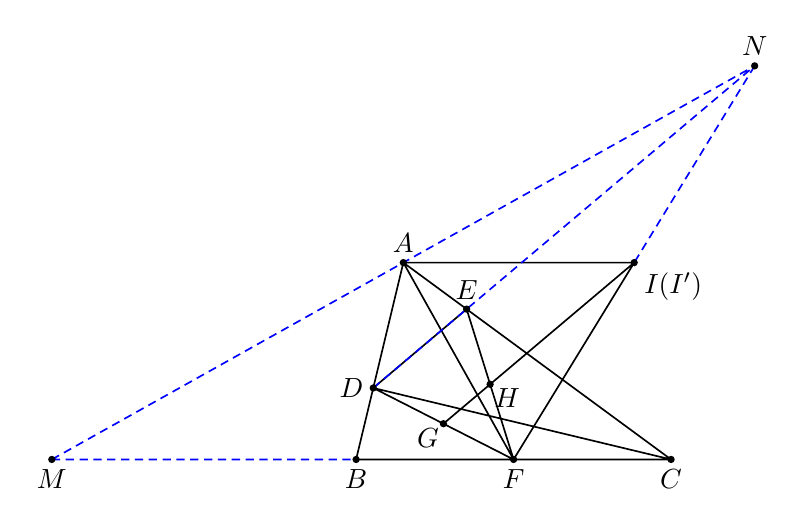
\begin{tikzpicture}[semithick]
\tkzDefPoints{0/0/B,4/0/C,0.6/2.5/A,2/2.5/I}
\tkzDefMidPoint(B,C)\tkzGetPoint{F}
\coordinate(D)at($(A)!(C)!(B)$);
\coordinate(E)at($(A)!(B)!(C)$);
\tkzDefMidPoint(F,D)\tkzGetPoint{G}
\tkzDefMidPoint(F,E)\tkzGetPoint{H}
\tkzInterLL(A,I)(G,H)\tkzGetPoint{I}
\draw(A)--(I)(A)--(B)(B)--(C)(C)--(A)(D)--(E)(D)--(C)
(E)--(F)(D)--(F)(G)--(I)(A)--(F)(I)--(F);
\tkzDefLine[orthogonal=through A](A,F)
\tkzGetPoint{A1}
\tkzInterLL(A,A1)(B,C)\tkzGetPoint{M}
\tkzInterLL(A,A1)(D,E)\tkzGetPoint{N}
\draw[densely dashed,blue](M)--(N)(M)--(B)(D)--(N)(N)--(I);
\tkzLabelPoints[below](B,F,C,M)
\tkzLabelPoints[above](A,E,N)
\tkzLabelPoints[left](D)
\node[below right]at(I){$I(I')$};
\tkzLabelPoints[below left=-1mm](G)
\tkzLabelPoints[below right=-1mm](H)
\tkzDrawPoints[size=2,fill=black](A,B,C,D,E,F,G,H,I,M,N)
\end{tikzpicture}
}
\caption{第 \thefigure 题图}
\end{figure}
\begin{Proof}
如图 \subref{20.2}, 显然$B,C,D,E$四点共圆,且圆心为点$F$.过点$A$作$AF$的垂线,交$CB$于$M$,交$DE$于$N$,根据蝴蝶定理知$AM=AN$,从而$\triangle AFM\qd \triangle AFN$,所以$\angle AFM=\angle AFN$.

 设$GH$交$FN$于$I'$,因为$GH\pxx DE$,所以$I$是$FN$的中点, $AI'=FI'$,所以$\angle I'AF=\angle I'FA=\angle MFA$,所以$AI'\pxx BC$,于是知$I'$与$I$重合为一点,所以$AI=FI$.
\end{Proof}
\item 如图 \subref{21.1}, $D$是$\triangle ABC$边$BC$上一点,使得$\angle DAC=\angle ABD$, $\odot O$过点$B,D$分别交$AB,AD$于点$E,F$,直线$BF$交$DE$于点$G$,求证: $CM\bot AO$.(2009年国家集训队选拔考试试题)
\begin{figure}[!ht]
\centering
\subfloat[]{\label{21.1}
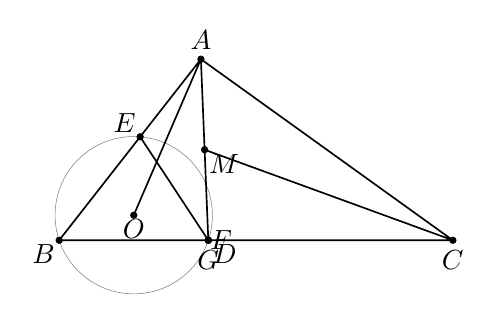
\begin{tikzpicture}[semithick]
\tkzInit[xmin=-0.4,xmax=5.2,ymin=-0.8,ymax=2.7]
\tkzClip
\tkzDefPoints{0/0/B,5/0/C,1.8/2.3/A}
\tkzDefMidPoint(A,C)\tkzGetPoint{K}
\tkzFindAngle(A,B,C)\tkzGetAngle{ABC}
\tkzDefPointBy[rotation=center A angle \ABC](K)
\tkzGetPoint{K1}
\tkzInterLL(A,K1)(B,C)\tkzGetPoint{D}
\tkzDefBarycentricPoint(A=2,B=1.5)\tkzGetPoint{E}
\tkzCircumCenter(B,D,E)\tkzGetPoint{O}
\tkzInterLC(A,D)(O,B)\tkzGetPoints{F}{F1}
\tkzInterLL(B,F)(D,E)\tkzGetPoint{G}
\tkzDefMidPoint(A,G)\tkzGetPoint{M}
\tkzDrawCircle(O,B)
\draw(A)--(B)(B)--(C)(A)--(C)(A)--(C)(A)--(G)(B)--(F)(D)--(E)(A)--(O)(A)--(D)
(C)--(M);
\tkzDrawPoints[size=2,fill=black](A,B,C,D,E,F,O,G,M)
\tkzLabelPoints[above](A)
\tkzLabelPoints[below right=-1mm](M,D)
\tkzLabelPoints[above left=-1mm](E)
\tkzLabelPoints[right=-1mm](F)
\tkzLabelPoints[below left=-1mm](B)
\tkzLabelPoints[below](C,G)
\tkzLabelPoints[below=-0.7mm](O)
\end{tikzpicture}
}
\subfloat[]{\label{21.2}
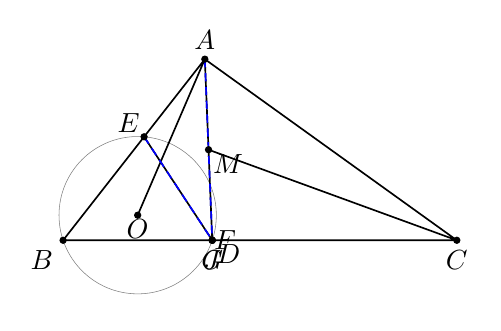
\begin{tikzpicture}[semithick]
\tkzInit[xmin=-0.45,xmax=5.2,ymin=-0.8,ymax=2.7]
\tkzClip
\tkzDefPoints{0/0/B,5/0/C,1.8/2.3/A}
\tkzDefMidPoint(A,C)\tkzGetPoint{K}
\tkzFindAngle(A,B,C)\tkzGetAngle{ABC}
\tkzDefPointBy[rotation=center A angle \ABC](K)
\tkzGetPoint{K1}
\tkzInterLL(A,K1)(B,C)\tkzGetPoint{D}
\tkzDefBarycentricPoint(A=2,B=1.5)\tkzGetPoint{E}
\tkzCircumCenter(B,D,E)\tkzGetPoint{O}
\tkzInterLC(A,D)(O,B)\tkzGetPoints{F}{F1}
\tkzInterLL(B,F)(D,E)\tkzGetPoint{G}
\tkzDefMidPoint(A,G)\tkzGetPoint{M}
\tkzDrawCircle(O,B)
\draw(A)--(B)(B)--(C)(A)--(C)(A)--(C)(A)--(G)(B)--(F)(D)--(E)(A)--(O)(A)--(D)
(C)--(M);
\tkzInterLL(E,F)(B,C)\tkzGetPoint{J}
\tkzInterLL(A,G)(B,C)\tkzGetPoint{I}
\draw[densely dashed,blue](E)--(J)(A)--(J)(J)--(G)(G)--(I);
\tkzDrawPoints[size=2,fill=black](A,B,C,D,E,F,O,G,M)
\tkzLabelPoints[above](A)
\tkzLabelPoints[below right=-1mm](M,D)
\tkzLabelPoints[above left=-1mm](E)
\tkzLabelPoints[right=-1mm](F)
\tkzLabelPoints[below left](B)
\tkzLabelPoints[below](C,G,J)
\tkzLabelPoints[below=-0.7mm](O)
\end{tikzpicture}
}
\subfloat[]{\label{21.3}
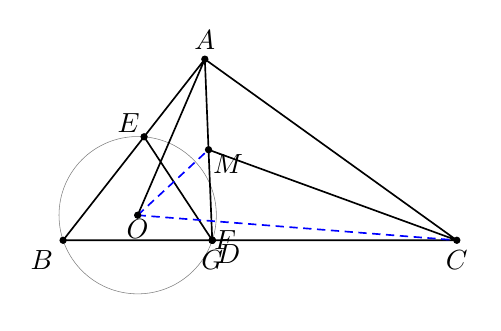
\begin{tikzpicture}[semithick]
\tkzInit[xmin=-0.45,xmax=5.2,ymin=-0.8,ymax=2.7]
\tkzClip
\tkzDefPoints{0/0/B,5/0/C,1.8/2.3/A}
\tkzDefMidPoint(A,C)\tkzGetPoint{K}
\tkzFindAngle(A,B,C)\tkzGetAngle{ABC}
\tkzDefPointBy[rotation=center A angle \ABC](K)
\tkzGetPoint{K1}
\tkzInterLL(A,K1)(B,C)\tkzGetPoint{D}
\tkzDefBarycentricPoint(A=2,B=1.5)\tkzGetPoint{E}
\tkzCircumCenter(B,D,E)\tkzGetPoint{O}
\tkzInterLC(A,D)(O,B)\tkzGetPoints{F}{F1}
\tkzInterLL(B,F)(D,E)\tkzGetPoint{G}
\tkzDefMidPoint(A,G)\tkzGetPoint{M}
\tkzDrawCircle(O,B)
\draw(A)--(B)(B)--(C)(A)--(C)(A)--(C)(A)--(G)(B)--(F)(D)--(E)(A)--(O)(A)--(D)
(C)--(M);
\draw[densely dashed,blue](O)--(C)(O)--(M);
\tkzDrawPoints[size=2,fill=black](A,B,C,D,E,F,O,G,M)
\tkzLabelPoints[above](A)
\tkzLabelPoints[below right=-1mm](M,D)
\tkzLabelPoints[above left=-1mm](E)
\tkzLabelPoints[right=-1mm](F)
\tkzLabelPoints[below left](B)
\tkzLabelPoints[below](C,G)
\tkzLabelPoints[below=-0.7mm](O)
\end{tikzpicture}
}
\caption{第 \thefigure 题图}
\end{figure}
\begin{Proof}
{\kaishu 方法一\quad}如图 \subref{21.2}, 连接$EF$并延长交$BC$于点$J$,延长$AG$交$BD$于点$I$,交$EF$于$H$.连接$AJ,CJ$,则知直线$GK$为点$A$关于$\odot O$的极线,于是知$JG\bot AO$.

 又$\angle DAC=\angle ABD=\angle DFJ$,所以$HJ\pxx AC$,所以$\frac{IH}{IA}=\frac{IJ}{IC}$.

 又在完全四边形$BDFEJA$中, 知$(AGHI)$是一组调和点列.又$M$是$AG$的中点,所以$IG\cdot IA=IH\cdot IM$,即$\frac{IG}{IM}=\frac{IH}{IA}=\frac{IJ}{IC}$,于是知$CM\pxx JG$,所以$CM\bot AO$.

{\kaishu 方法二\quad}如图 \subref{21.3}, 因为$A,G$为一对共轭点,故$M$关于$\odot O$的幂为$MA^2$,于是知$MO^2-MA^2=R^2=CO^2-CD\cdot CB=CO^2-CA^2$,从而$CM\bot AO$.
\end{Proof}
\item 如图 \subref{22.1}, $CD$为$\odot O$的直径, $PC,PE$分别切$\odot O$于$C,E$,割线$PBA$交$\odot O$于$A,B$, $AC,BD$交于点$F$, $DE$交$AB$于$G$,求证: $\angle GFE=\angle ADE$.
\begin{figure}[!ht]
\centering
\subfloat[]{\label{22.1}
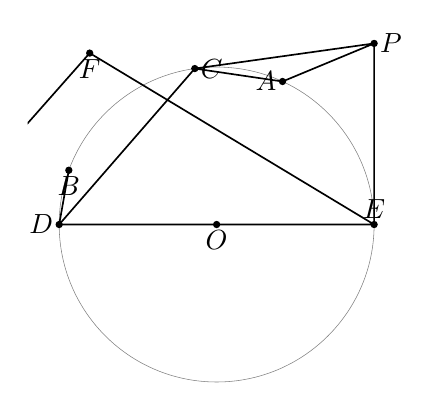
\begin{tikzpicture}[semithick]
\tkzInit[xmin=-2.4,xmax=2.4,ymin=-2.1,ymax=2.5]
\tkzClip
\tkzDefPoints{-2/0/D,2/0/C,2/2.3/P,-1.3/0/K}
\tkzDefMidPoint(D,C)\tkzGetPoint{O}
\tkzTangent[from=P](O,C)\tkzGetPoints{E}{C}
\tkzDrawCircle(O,C)
\tkzInterCC(O,C)(D,K)\tkzGetSecondPoint{A}
\tkzInterLC(P,A)(O,C)\tkzGetPoints{A}{B}
\tkzInterLL(A,C)(B,D)\tkzGetPoint{F}
\tkzInterLL(A,B)(D,E)\tkzGetPoint{G}
\draw[semithick](D)--(C)(C)--(P)(P)--(E)(E)--(D)(P)--(A)(F)--(G)(A)--(C)
(D)--(B)(F)--(E);
\tkzLabelPoints[left=-0.5mm](A,D)
\tkzLabelPoints[right=-0.5mm](C,P)
\tkzLabelPoints[below=-0.5mm](O,B,F)
\tkzLabelPoints[above=-0.5mm](E)
\tkzLabelPoints[above left=-1mm](G)
\tkzDrawPoints[size=2,fill=black](A,C,D,O,P,E,B,F,G)
\end{tikzpicture}
}\hspace{2cm}
\subfloat[]{\label{22.2}
\begin{tikzpicture}[semithick]
\tkzInit[xmin=-3.8,xmax=2.4,ymin=-2.1,ymax=2.5]
\tkzClip
\tkzDefPoints{-2/0/D,2/0/C,2/2.3/P,-1.3/0/K}
\tkzDefMidPoint(D,C)\tkzGetPoint{O}
\tkzTangent[from=P](O,C)\tkzGetPoints{E}{C}
\tkzDrawCircle(O,C)
\tkzInterCC(O,C)(D,K)\tkzGetSecondPoint{A}
\tkzInterLC(P,A)(O,C)\tkzGetPoints{A}{B}
\tkzInterLL(A,C)(B,D)\tkzGetPoint{F}
\tkzInterLL(A,B)(D,E)\tkzGetPoint{G}
\draw[semithick](D)--(C)(C)--(P)(P)--(E)(E)--(D)(P)--(A)(F)--(G)(A)--(C)
(D)--(B)(F)--(E);
\tkzInterLL(P,A)(C,D)\tkzGetPoint{H}
\draw[densely dashed,semithick,blue](A)--(H)(H)--(D)(A)--(E)(E)--(B)(B)--(C);
\tkzLabelPoints[below left=-0.7mm](D)
\tkzLabelPoints[right=-0.5mm](C,P)
\tkzLabelPoints[below=-0.5mm](O,B,H,F)
\tkzLabelPoints[above=-0.5mm](E)
\tkzLabelPoints[above left=-1mm](A,G)
\tkzDrawPoints[size=2,fill=black](A,C,D,O,P,E,B,F,G,H)
\end{tikzpicture}
}
\caption{第 \thefigure 题图}
\end{figure}
\begin{Proof}
如图 \subref{22.2},延长$PA$交$CD$于$H$,连接$AE,BE,BC$,因为四边形$AEBC$是调和四边形,所以$DA,DB,DE,DC$是一组调和线束,从而$H,G,A,B$是一组调和点列,于是知$G$在$H$关于$\odot O$的极线上.又$F$在$H$关于$\odot O$的极线上,所以直线$GF$是$H$关于$\odot O$的极线,于是知$GF\bot CD$.从而知
\[\angle GFB=90^\circ-\angle FDC=\angle DCB=180^\circ-\angle GEB,\]
所以$G,F,B,E$四点共圆,于是知$\angle GFE=\angle GBE=\angle ADE$.
\end{Proof}
\item 如图 \subref{23.1}, $O$为$\triangle ABC$的外心, $D,E$分别为$AB,AC$上一点, $OF\bot DE$于$F$, $L,M,N$分别为$DE,BE,CD$的中点,求证: $F,L,M,N$四点共圆.
\begin{figure}[!ht]
\centering
\subfloat[]{\label{23.1}
\begin{tikzpicture}[inner sep=2pt,semithick]
\tkzInit[xmin=-0.3,xmax=4.3,ymin=-0.5,ymax=4.8]
\tkzClip
\tkzDefPoints{0/0/B,4/0/C,3/4.3/A}
\tkzDefBarycentricPoint(A=1.8,B=1)\tkzGetPoint{D}
\tkzDefBarycentricPoint(A=1.3,C=1)\tkzGetPoint{E}
\tkzCircumCenter(A,B,C)\tkzGetPoint{O}
\coordinate(F)at($(D)!(O)!(E)$);
\tkzDefMidPoint(C,D)\tkzGetPoint{N}
\tkzDefMidPoint(B,E)\tkzGetPoint{M}
\tkzDefMidPoint(D,E)\tkzGetPoint{L}
\draw(A)--(B)(B)--(C)(C)--(A)(D)--(E)(B)--(E)(C)--(D)
(O)--(F);
\tkzLabelPoints[below](B,C)\tkzLabelPoints[above](A)
\tkzLabelPoints[left](D,O)\tkzLabelPoints[below right](M)
\tkzLabelPoints[right](E)\tkzLabelPoints[below left](N)
\tkzLabelPoints[above right](L,F)
\tkzDrawPoints[size=2,fill=black](A,B,C,D,E,F,O,L,M,N)
\end{tikzpicture}
}\hspace{2cm}
\subfloat[]{\label{23.2}
\begin{tikzpicture}[inner sep=2pt,semithick]
\tkzInit[xmin=-0.3,xmax=4.3,ymin=-0.5,ymax=4.8]
\tkzClip
\tkzDefPoints{0/0/B,4/0/C,3/4.3/A}
\tkzDefBarycentricPoint(A=1.8,B=1)\tkzGetPoint{D}
\tkzDefBarycentricPoint(A=1.3,C=1)\tkzGetPoint{E}
\tkzCircumCenter(A,B,C)\tkzGetPoint{O}
\coordinate(F)at($(D)!(O)!(E)$);
\tkzDefMidPoint(C,D)\tkzGetPoint{N}
\tkzDefMidPoint(B,E)\tkzGetPoint{M}
\tkzDefMidPoint(D,E)\tkzGetPoint{L}
\draw(A)--(B)(B)--(C)(C)--(A)(D)--(E)(B)--(E)(C)--(D)
(O)--(F)(F)--(M)(F)--(N);
\tkzLabelPoints[below](B,C)\tkzLabelPoints[above](A)
\tkzLabelPoints[left](D)\tkzLabelPoints[below right](M)
\tkzLabelPoints[right](O,E)\tkzLabelPoints[below left](N)
\tkzLabelPoints[above right](F)
\tkzDrawPoints[size=2,fill=black](A,B,C,D,E,F,O,M,N)
\end{tikzpicture}
}\\
\subfloat[]{\label{23.3}
\begin{tikzpicture}[inner sep=2pt,semithick]
\tkzInit[xmin=-1,xmax=5,ymin=-1,ymax=4.8]
\tkzClip
\tkzDefPoints{0/0/B,4/0/C,3/4.3/A}
\tkzDefBarycentricPoint(A=1.8,B=1)\tkzGetPoint{D}
\tkzDefBarycentricPoint(A=1.3,C=1)\tkzGetPoint{E}
\tkzCircumCenter(A,B,C)\tkzGetPoint{O}
\coordinate(F)at($(D)!(O)!(E)$);
\tkzDefMidPoint(C,D)\tkzGetPoint{N}
\tkzDefMidPoint(B,E)\tkzGetPoint{M}
\tkzDefMidPoint(D,E)\tkzGetPoint{L}
\draw[semithick](A)--(B)(B)--(C)(C)--(A)(D)--(E)(B)--(E)(C)--(D)
(O)--(F)(F)--(M)(F)--(N);
\begin{scope}[densely dashed,blue]
\tkzDrawCircle[densely dashed,draw=blue](O,A)
\tkzInterLC(B,F)(O,A)\tkzGetPoints{B}{I}
\tkzInterLC(C,F)(O,A)\tkzGetPoints{J}{C}
\tkzInterLL(J,D)(I,E)\tkzGetPoint{K}
\tkzInterLC(K,F)(O,A)\tkzGetPoints{T}{K}
\tkzInterLL(T,B)(D,E)\tkzGetPoint{P}
\tkzInterLL(T,C)(D,E)\tkzGetPoint{Q}
\draw(B)--(I)(C)--(J)(I)--(K)(J)--(K)(K)--(T)(T)--(B)(T)--(C)
(B)--(J)(C)--(I);
\end{scope}
\tkzLabelPoints[above](A,T)\tkzLabelPoints[above left](J)
\tkzLabelPoints[left](D,P)\tkzLabelPoints[below right](M,C,K)
\tkzLabelPoints[right](O,E)\tkzLabelPoints[below left](N,B)
\tkzLabelPoints[above right](F,I,Q)
\tkzDrawPoints[size=2,fill=black](A,B,C,D,E,F,O,M,N,I,J,K,T,P,Q)
\end{tikzpicture}
}\hspace{0.6cm}
\subfloat[]{\label{23.4}
\begin{tikzpicture}[inner sep=2pt,semithick]
\tkzInit[xmin=-1,xmax=5,ymin=-1,ymax=4.8]
\tkzClip
\tkzDefPoints{0/0/B,4/0/C,3/4.3/A}
\tkzDefBarycentricPoint(A=1.8,B=1)\tkzGetPoint{D}
\tkzDefBarycentricPoint(A=1.3,C=1)\tkzGetPoint{E}
\tkzCircumCenter(A,B,C)\tkzGetPoint{O}
\coordinate(F)at($(D)!(O)!(E)$);
\tkzDefMidPoint(C,D)\tkzGetPoint{N}
\tkzDefMidPoint(B,E)\tkzGetPoint{M}
\tkzDefMidPoint(D,E)\tkzGetPoint{L}
\draw(A)--(B)(B)--(C)(C)--(A)(D)--(E)(B)--(E)(C)--(D)
(O)--(F);
\tkzDrawCircle[densely dashed,draw=blue](O,A)
\draw[densely dashed,color=blue](M)--(F)(M)--(L)(L)--(N)(F)--(N);
\tkzLabelPoints[above](A)
\tkzLabelPoints[left](D,O)\tkzLabelPoints[below right](M,C)
\tkzLabelPoints[right](E)\tkzLabelPoints[below left](B,N)
\tkzLabelPoints[above right](L,F)
\tkzDrawPoints[size=2,fill=black](A,B,C,D,E,F,O,L,M,N)
\end{tikzpicture}
}
\caption{第 \thefigure 题图}
\end{figure}
\begin{proof}
我们先证明一个引理: 如图 \subref{23.2}, $O$为$\triangle ABC$的外心, $D,E$分别为$AB,AC$上一点, $OF\bot DE$于$F$. $M,N$分别为$BE,CD$的中点,则$\angle MFN=\angle A$.

\textbf{引理的证明}: 如图 \subref{23.3}, 作$\triangle ABC$的外接圆$\odot O$,分别延长$BF,CF$交$\odot O$于$I,J$,延长$JD,IE$交于点$K$,根据帕斯卡定理知$K$在$\odot O$上.延长$KF$交$\odot O$于$T$,连接$TB$交$DE$于$P$,连接$TC$交$DE$于$Q$.根据蝴蝶定理: $FP=FE,FD=FQ$.由中位线定理知$MF\pxx BP,NF\pxx CE$,所以$\angle MFN=\angle BTC=\angle BAC$.

 下面借助引理证明原命题.
\quad  如图 \subref{23.4},连接$MF,NF,ML,NL$,根据引理知$\angle MFN=\angle A$.又因为$ML\pxx BD,NL\pxx CF$,所以$\angle MLN=\angle A$.于是$\angle MFN=\angle MLN$,所以$F,L,M,N$四点共圆.
\end{proof} 
\setcounter{enumi}{41}
\setcounter{figure}{41}
\item 如图 \subref{42.1}, $AB$为半圆$O$的直径, $OC\bot AB$, $C$在圆上, $P$是$BA$延长线上一点, $PD$切$\odot O$于$D$, $PE$平分$\angle DPB$,分别交$AC,BC$于$E,F$,求证: $\angle EOF=90^\circ$.(2007年辽宁高中数学竞赛)
\begin{figure}[!ht]
\centering
\subfloat[]{\label{42.1}
\begin{tikzpicture}[semithick,inner sep=1.5pt]
\tkzInit[xmin=-0.2,xmax=5.4,ymin=-0.4,ymax=2.4]
\tkzClip
\tkzDefPoints{0/0/P,1.2/0/A,5.2/0/B,3.2/0/O,3.2/2/C}
\tkzDrawArc[draw=black,semithick](O,B)(A)
\tkzTangent[from=P](O,A)\tkzGetSecondPoint{D}
\tkzDefLine[bisector](D,P,A)\tkzGetPoint{E}
\tkzInterLL(P,E)(A,C)\tkzGetPoint{E}
\tkzInterLL(P,E)(C,B)\tkzGetPoint{F}
\tkzLabelPoints[above](C)
\tkzLabelPoints[above left](D)
\tkzLabelPoints[below](P,A,O,B,E)
\tkzLabelPoints[above right](F)
\draw(P)--(D)(P)--(B)(A)--(C)(C)--(B)(O)--(E)(O)--(F)(P)--(F);
\tkzDrawPoints[size=2,fill=black](A,B,C,D,E,F,O,P)
\end{tikzpicture}
}
\subfloat[]{\label{42.2}
\begin{tikzpicture}[semithick,inner sep=1.5pt]
\tkzInit[xmin=-0.2,xmax=5.4,ymin=-0.4,ymax=2.4]
\tkzClip
\tkzDefPoints{0/0/P,1.2/0/A,5.2/0/B,3.2/0/O,3.2/2/C}
\tkzDrawArc[draw=black,semithick](O,B)(A)
\tkzTangent[from=P](O,A)\tkzGetSecondPoint{D}
\tkzDefLine[bisector](D,P,A)\tkzGetPoint{E}
\tkzInterLL(P,E)(A,C)\tkzGetPoint{E}
\tkzInterLL(P,E)(C,B)\tkzGetPoint{F}
\draw[fuzhu](A)--(D)--(E)(D)--(O)(D)--(B)(D)--(C)(D)--(F);
\tkzLabelPoints[above](C)
\tkzLabelPoints[above left](D)
\tkzLabelPoints[below](P,A,O,B,E)
\tkzLabelPoints[above right](F)
\draw(P)--(D)(P)--(B)(A)--(C)(C)--(B)(O)--(E)(O)--(F)(P)--(F);
\tkzDrawPoints[size=2,fill=black](A,B,C,D,E,F,O,P)
\end{tikzpicture}
}
\caption{第 \thefigure 题图}
\end{figure}
\begin{proof}
如图 \subref{42.2}, 连接$DA,DE,DO,DB,DF,DC$,则
\begin{align*}
\angle DPE&=\frac12\angle DPO=\frac12(90^\circ-\angle DOA)=45^\circ-\angle DBA\\
&=\angle ABC-\angle ABD=\angle DBC=\angle DAC,
\end{align*}
所以$D,P,A,E$四点共圆, $P,D,F,B$四点共圆.注意到$AF$平分$\angle DAB$,因此$AE=DE,BF=DF$.又$OA=OD=OB$,所以$OE\bot AD,OF\bot BD$,因此$OE\bot OF$,即$\angle EOF=90^\circ$.
\end{proof}
\item 如图 \subref{43.1}, $PA$为$\odot O$, $PBC$为$\odot O$的割线, $AD\bot OP$于$D$, $\triangle ADC$的外接圆与$BC$的另一个交点为$E$,证明: $\angle BAE=\angle ACB$.(2012年初中数学联赛二试试题)
\begin{figure}[!ht]
\centering
\subfloat[]{\label{43.1}
\begin{tikzpicture}[semithick,inner sep=1.5pt]
\tkzInit[xmin=-0.4,xmax=5,ymin=-1.3,ymax=1.9]
\tkzClip
\tkzDefPoints{0/0/P,3/0/O,1.8/-0.3/B}
\tkzTangent[from=P](O,B)\tkzGetPoints{A1}{A}
\tkzDrawCircle(O,B)
\coordinate(D)at($(P)!(A)!(O)$);
\tkzInterLC(P,B)(O,B)\tkzGetPoints{C}{B}
\tkzCircumCenter(A,D,C)\tkzGetPoint{Q}
\tkzDrawCircle(Q,A)
\tkzInterLC(B,C)(Q,A)\tkzGetPoints{C}{E}
\draw(A)--(P)(P)--(O)(A)--(D)(A)--(B)(P)--(C)(A)--(C)(C)--(D)(A)--(E);

\tkzLabelPoints[above left](A)
\tkzLabelPoints[left](P)
\tkzLabelPoints[right,inner sep=1pt](O)
\tkzLabelPoints[below left](B,E,D)
\tkzLabelPoints[below right](C)
\tkzDrawPoints[size=2,fill=black](A,P,D,O,B,E,C)
\end{tikzpicture}
}
\subfloat[]{\label{43.2}
\begin{tikzpicture}[semithick,inner sep=1.5pt]
\tkzInit[xmin=-0.4,xmax=5,ymin=-1.3,ymax=1.9]
\tkzClip
\tkzDefPoints{0/0/P,3/0/O,1.8/-0.3/B}
\tkzTangent[from=P](O,B)\tkzGetPoints{A1}{A}
\tkzDrawCircle(O,B)
\coordinate(D)at($(P)!(A)!(O)$);
\tkzInterLC(P,B)(O,B)\tkzGetPoints{C}{B}
\tkzCircumCenter(A,D,C)\tkzGetPoint{Q}
\tkzDrawCircle(Q,A)
\tkzInterLC(B,C)(Q,A)\tkzGetPoints{C}{E}
\draw(A)--(P)(P)--(O)(A)--(D)(A)--(B)(P)--(C)(A)--(C)(C)--(D)(A)--(E);
\draw[fuzhu](A)--(O)(O)--(C)(D)--(B)(O)--(B)(D)--(C);
\tkzLabelPoints[above left](A)
\tkzLabelPoints[left](P)
\tkzLabelPoints[right](O)
\tkzLabelPoints[below left](B,E,D)
\tkzLabelPoints[below right](C)
\tkzDrawPoints[size=2,fill=black](A,P,D,O,B,E,C)
\end{tikzpicture}
}
\caption{第 \thefigure 题图}
\end{figure}
\begin{proof}
如图 \subref{43.2}, 连接$OA,OB,OC,BD,CD$.因为$OA\bot PA$,根据射影定理知$PA^2=PD\cdot PO$.又根据切割线定理知$PA^2=PB\cdot PC$,所以$PD\cdot PO=PB\cdot PC$,因此$B,D,O,C$四点共圆.于是知
\begin{align*}
 \angle BEA&=180^\circ-\angle AEC=180^\circ-\angle ADC\\
&=90^\circ-\angle CDO=90^\circ-\angle CBO=\angle BAC,
\end{align*}
因此$\triangle ABE\xs\triangle CBA$,所以$\angle BAE=\angle ACB$.
\end{proof}
\item 如图 \subref{44.1}, $\pxsbx ABCD$中, $CE\bot AB$于$E$, $CF\bot AD$于$F$, $EF$交$BD$于$G$,求证$GC\bot AC$.
\begin{figure}[!ht]
\centering
\subfloat[]{\label{44.1}
\begin{tikzpicture}[semithick,inner sep=1.5pt]
\tkzDefPoints{0/0/B,3/0/C,0.5/1.8/A,3.5/1.8/D}
\coordinate(E)at($(A)!(C)!(B)$);
\coordinate(F)at($(A)!(C)!(D)$);
\tkzInterLL(E,F)(B,D)\tkzGetPoint{G}
\draw(A)--(B)--(C)--(D)--(A)--(C)(B)--(G)--(E)--(C)--(G)(C)--(F);
\tkzLabelPoints[above](A,F)
\tkzLabelPoints[below](B,C)
\tkzLabelPoints[left](E)
\tkzLabelPoints[below right](D)
\tkzLabelPoints[right](G)
\tkzDrawPoints[size=2,fill=black](A,B,C,D,E,F,G)
\end{tikzpicture}
}
\subfloat[]{\label{44.2}
\begin{tikzpicture}[semithick,inner sep=1.5pt]
\tkzDefPoints{0/0/B,3/0/C,0.5/1.8/A,3.5/1.8/D}
\coordinate(E)at($(A)!(C)!(B)$);
\coordinate(F)at($(A)!(C)!(D)$);
\tkzInterLL(E,F)(B,D)\tkzGetPoint{G}
\draw(A)--(B)--(C)--(D)--(A)--(C)(B)--(G)--(E)--(C)--(G)(C)--(F);
\tkzDefMidPoint(A,C)\tkzGetPoint{O}
\tkzDrawCircle[densely dashed,draw=blue](O,A)
\tkzDefLine[parallel=through E](B,D)
\tkzGetPoint{E1}
\tkzInterLL(E,E1)(A,D)\tkzGetPoint{M}
\tkzInterLL(E,M)(A,C)\tkzGetPoint{N}
\coordinate(K)at($(E)!(O)!(G)$);
\draw[fuzhu](E)--(M)(N)--(K)--(O)(K)--(C);
\tkzLabelPoints[above](F,M,K)
\tkzLabelPoints[below](B,O)
\tkzLabelPoints[left](E)
\tkzLabelPoints[above left](A)
\tkzLabelPoints[below right](D,C)
\tkzLabelPoints[right](G)
\tkzDrawPoints[size=2,fill=black](A,B,C,D,E,F,G,O,M,K)
\end{tikzpicture}
}
\caption{第 \thefigure 题图}
\end{figure}
\begin{proof}
如图 \subref{44.2}, 设$AC,BD$交于点$O$,则$O$为$BD$的中点.根据条件知$C,E,A,F$四点共圆,圆心为$O$,作四边形$CEAF$的外接圆$\odot O$.过$E$作$EM\pxx BD$,交$AD$于$M$,交$AC$于$N$.因为$O$为$BD$的中点,所以$N$为$EM$的中点.过$O$作$OK\bot EF$,根据垂径定理知$K$为$EF$的中点,所以$NK\pxx MF$,于是知$\angle NKE=\angle AFE=\angle ACE$,所以$E,N,K,C$四点共圆,所以$\angle KCO=\angle KEN=\angle KGO$,所以$O,K,G,C$四点共圆,所以$\angle OCG=180^\circ-\angle OKG=90^\circ$,所以$GC\bot AC$.
\end{proof}
\item 如图 \subref{45.1}, $\triangle ABC$内接于$\odot O,AD\bot BC$于$D$, $AD$交$CO$于$E$, $F$为$AE$的中点, $FO$交$BC$于$H$, $CG\bot AO$于$G$,求证: $B,H,O,G$四点共圆.
\begin{figure}[!ht]
\centering
\subfloat[]{\label{45.1}
\begin{tikzpicture}[semithick,inner sep=1.5pt]
\tkzInit[xmin=-0.4,xmax=4.4,ymin=-1.4,ymax=3.1]
\tkzClip
\tkzDefPoints{0/0/B,4/0/C,3.1/2.7/A}
\coordinate(D)at($(B)!(A)!(C)$);
\tkzCircumCenter(A,B,C)\tkzGetPoint{O}
\tkzInterLL(A,D)(C,O)\tkzGetPoint{E}
\coordinate(F)at($(A)!0.5!(E)$);
\coordinate(G)at($(A)!(C)!(O)$);
\tkzInterLL(F,O)(B,C)\tkzGetPoint{H}
\tkzDrawCircle(O,A)
\draw(A)--(B)--(C)--(A)--(D)(O)--(C)(F)--(H)(G)--(C)(G)--(B)(A)--(O);
\tkzLabelPoints[below left](B,E)
\tkzLabelPoints[below](H,D)
\tkzLabelPoints[below right](C)
\tkzLabelPoints[above left](G)
\tkzLabelPoints[right](F)
\tkzLabelPoints[below](O)
\tkzLabelPoints[above](A)
\tkzDrawPoints[size=2,fill=black](A,B,C,D,E,F,O,G,H)

\end{tikzpicture}
}\hspace{2cm}
\subfloat[]{\label{45.2}
\begin{tikzpicture}[semithick,inner sep=1.5pt]
\tkzInit[xmin=-0.4,xmax=4.4,ymin=-1.4,ymax=3.1]
\tkzClip
\tkzDefPoints{0/0/B,4/0/C,3.1/2.7/A}
\coordinate(D)at($(B)!(A)!(C)$);
\tkzCircumCenter(A,B,C)\tkzGetPoint{O}
\tkzInterLL(A,D)(C,O)\tkzGetPoint{E}
\coordinate(F)at($(A)!0.5!(E)$);
\coordinate(G)at($(A)!(C)!(O)$);
\tkzInterLL(F,O)(B,C)\tkzGetPoint{H}
\tkzDrawCircle(O,A)
\draw(A)--(B)--(C)--(A)--(D)(O)--(C)(F)--(H)(G)--(C)(G)--(B)(A)--(O);
\tkzDefPointBy[rotation=center O angle 180](A)
\tkzGetPoint{J}
\draw[fuzhu](B)--(J)--(E)(J)--(O)(J)--(C);
\tkzLabelPoints[below left](B,E,J)
\tkzLabelPoints[below](H,D)
\tkzLabelPoints[below right](C)
\tkzLabelPoints[above left](G)
\tkzLabelPoints[right](F)
\tkzLabelPoints[below](O)
\tkzLabelPoints[above](A)
\tkzDrawPoints[size=2,fill=black](A,B,C,D,E,F,O,G,H,J)

\end{tikzpicture}
}

\subfloat[]{\label{45.3}
\begin{tikzpicture}[semithick,inner sep=1.5pt]
\tkzInit[xmin=-0.4,xmax=4.4,ymin=-3,ymax=3.1]
\tkzClip
\tkzDefPoints{0/0/B,4/0/C,3.1/2.7/A}
\coordinate(D)at($(B)!(A)!(C)$);
\tkzCircumCenter(A,B,C)\tkzGetPoint{O}
\tkzInterLL(A,D)(C,O)\tkzGetPoint{E}
\coordinate(F)at($(A)!0.5!(E)$);
\coordinate(G)at($(A)!(C)!(O)$);
\tkzInterLL(F,O)(B,C)\tkzGetPoint{H}
\tkzDrawCircle(O,A)
\draw(A)--(B)--(C)--(A)--(D)(O)--(C)(F)--(H)(G)--(C)(G)--(B)(A)--(O);
\tkzInterLC(C,G)(O,C)\tkzGetPoints{K}{C}
\draw[fuzhu](B)--(K)--(G);
\tkzLabelPoints[below left](B,E)
\tkzLabelPoints[below](H,D)
\tkzLabelPoints[below right](C)
\tkzLabelPoints[above left](K)
\tkzLabelPoints[right](F)
\tkzLabelPoints[below](O)
\tkzLabelPoints[above](A,G)
\tkzDrawPoints[size=2,fill=black](A,B,C,D,E,F,O,G,H,K)

\end{tikzpicture}
}\hspace{2cm}
\subfloat[]{\label{45.4}
\begin{tikzpicture}[semithick,inner sep=1.5pt]
\tkzInit[xmin=-0.4,xmax=4.4,ymin=-3,ymax=3.1]
\tkzClip
\tkzDefPoints{0/0/B,4/0/C,3.1/2.7/A}
\coordinate(D)at($(B)!(A)!(C)$);
\tkzCircumCenter(A,B,C)\tkzGetPoint{O}
\tkzInterLL(A,D)(C,O)\tkzGetPoint{E}
\coordinate(F)at($(A)!0.5!(E)$);
\coordinate(G)at($(A)!(C)!(O)$);
\tkzInterLL(F,O)(B,C)\tkzGetPoint{H}
\tkzDrawCircle(O,A)
\draw(A)--(B)--(C)--(A)--(D)(O)--(C)(F)--(H)(G)--(C)(G)--(B)(A)--(O);
\tkzDefPointBy[rotation=center O angle 180](C)\tkzGetPoint{J}
\tkzInterLL(J,B)(A,O)\tkzGetPoint{M}
\tkzInterLL(J,B)(F,H)\tkzGetPoint{K}
\draw[fuzhu](O)--(J)--(M)--(O)(C)--(M)(K)--(H);
\tkzLabelPoints[below left](E)
\tkzLabelPoints[below](H,D)
\tkzLabelPoints[below right](C)
\tkzLabelPoints[above left](J,G)
\tkzLabelPoints[right](F)
\tkzLabelPoints[below](O,M)
\tkzLabelPoints[above](A)
\tkzLabelPoints[left](K,B)
\tkzDrawPoints[size=2,fill=black](A,B,C,D,E,F,O,G,H,J,K,M)

\end{tikzpicture}
}
\caption{第 \thefigure 题图}
\end{figure}
\begin{proof}
{\kaishu 方法一\quad}如图 \subref{45.2}, 延长$AO$交$\odot O$于$J$,连接$EJ,BJ,CJ$.因为
\[\angle BCJ=\angle BAJ=\angle CAE,\angle CBJ=\angle CAJ=\angle ACE,\]
所以$\triangle BCJ\xs\triangle CAE$,所以
\[\frac{AE}{CJ}=\frac{AC}{BC}\Rightarrow AE\cdot BC=AC\cdot CJ=CG\cdot AJ\Rightarrow
\frac{AE}{CG}=\frac{AJ}{BC}.\]
又$\angle EAJ=\angle GCB$,所以$\triangle EAJ\xs\triangle GCB$,所以$\angle CJA=\angle GBH$.又$OF$为$\triangle AJE$的中位线,所以$OF\pxx JD$,故$\angle HOJ=\angle EJA=\angle GBH$,所以$B,H,O,G$四点共圆.

{\kaishu 方法二\quad}如图 \subref{45.3}, 延长$CG$交$\odot O$于$K$,则$G$为$CK$的中点,且$\angle KBC=2\angle ABC=\angle EOA$.又易知$A,G,D,C$四点共圆,则$\angle BCK=\angle OAE$,所以$\triangle CBK\xs\triangle AOE$.又注意到$F$为$AE$的中点, $G$为$CK$的中点,所以$\triangle CBG\xs\triangle AOF$,故$\angle CBG=\angle AOF$,所以$B,H,O,G$四点共圆.

{\kaishu 方法三\quad}如图 \subref{45.4}, 延长$CO$交$\odot O$于$J$,连接$JB$交$AO$的延长线于$M$,连接$CM$,延长$FH$交$JM$于$K$.因为$JM\bot BC,AD\bot BC$,所以$JM\pxx AD$,又$F$为$AE$的中点,所以$K$为$JM$的中点,所以$OK$为$\triangle JMC$的中位线,则$OK\pxx MC$.又显然$B,M,C,G$四点共圆,所以$\angle BGO=\angle BCM=\angle CHO$,所以$B,H,O,G$四点共圆.
\end{proof}
\item 如图 \subref{46.1}, $I$是$\triangle ABC$的内心, $A$关于$BC$的对称点为$K$, $E$为$BC$的中点, $F$为$\wideparen{BC}$的中点, $EF$的中点为$N$, $BI$的中点为$M$, $MN$交$BC$于$D$,求证: $A,K,D,M$四点共圆.
\begin{figure}[!ht]
\centering
\subfloat[]{\label{46.1}
\begin{tikzpicture}[semithick,inner sep=1.5pt]
\tkzDefPoints{0/0/B,4/0/C,3/4/A}
\tkzInit[xmin=-0.7,xmax=5.2,ymin=-1.3,ymax=4.4]
\tkzClip
\tkzInCenter(A,B,C)\tkzGetPoint{I}
\tkzCircumCenter(A,B,C)\tkzGetPoint{O}
\tkzDefPointBy[reflection=over B--I](A)
\tkzGetPoint{K}
\coordinate(E)at($(B)!0.5!(C)$);
\tkzDrawCircle(O,A)
\tkzInterLC(O,E)(O,B)\tkzGetPoints{F1}{F}
\coordinate(M)at($(B)!0.5!(I)$);
\coordinate(N)at($(E)!0.5!(F)$);
\tkzInterLL(M,N)(B,C)\tkzGetPoint{D}
\draw(A)--(B)--(C)--(A)(E)--(F)(M)--(N)(A)--(K)(B)--(I)(A)--(M);
\tkzLabelPoints[below](F,O,K)
\tkzLabelPoints[right](I,N)
\tkzLabelPoints[above left](M)
\tkzLabelPoints[below left](B,D)
\tkzLabelPoints[below right](C)
\tkzLabelPoints[right](N)
\tkzLabelPoints[above](E,A)
\tkzDrawPoints[size=2,fill=black](A,B,C,F,E,O,K,M,N,I,D)
\end{tikzpicture}
}
\subfloat[]{\label{46.2}
\begin{tikzpicture}[semithick,inner sep=1.5pt]
\tkzDefPoints{0/0/B,4/0/C,3/4/A}
\tkzInit[xmin=-0.7,xmax=5.2,ymin=-1.3,ymax=4.4]
\tkzClip
\tkzInCenter(A,B,C)\tkzGetPoint{I}
\tkzCircumCenter(A,B,C)\tkzGetPoint{O}
\tkzDefPointBy[reflection=over B--I](A)
\tkzGetPoint{K}
\coordinate(E)at($(B)!0.5!(C)$);
\tkzDrawCircle(O,A)
\tkzInterLC(O,E)(O,B)\tkzGetPoints{F1}{F}
\coordinate(M)at($(B)!0.5!(I)$);
\coordinate(N)at($(E)!0.5!(F)$);
\tkzInterLL(M,N)(B,C)\tkzGetPoint{D}
\draw(A)--(B)--(C)--(A)(E)--(F)(M)--(N)(A)--(K)(B)--(I)(A)--(M);
\draw[fuzhu](A)--(F)(M)--(E)(M)--(K)--(C)(B)--(F)--(M);
\tkzLabelPoints[below](F,O,K)
\tkzLabelPoints[right](I,N)
\tkzLabelPoints[above left](M)
\tkzLabelPoints[below left](B,D)
\tkzLabelPoints[below right](C)
\tkzLabelPoints[right](N)
\tkzLabelPoints[above](E,A)
\tkzDrawPoints[size=2,fill=black](A,B,C,F,E,O,K,M,N,I,D)
\end{tikzpicture}
}
\caption{第 \thefigure 题图}
\end{figure}
\begin{proof}
根据条件知$K$在直线$BC$上, 且$AB=KB$.连接$AF$,则$AF$过点$I$,且$FB=FI$.因为$M$为$BI$的中点,所以$FM\bot BI$,于是知$B,M,E,F$四点共圆,所以
\[\angle MFE=\angle EBI=\angle ABI,\angle FME=\angle FBC=\angle FAC=\angle BAI,\]
所以$\triangle MFE\xs\triangle ABI$.又$N,M$分别为$EF,BI$的中点,所以$\triangle MFN\xs\triangle ABM$,于是知$\angle FMN=\angle BAM$,所以
\begin{align*}
\angle DMA+\angle DKA&=(\angle FMA-\angle FMN)+\angle BAK\\
&=(\angle FMA-\angle BAM)+(\angle BAM+\angle MAK)\\
&=\angle FMA+\angle MAK.
\end{align*}
又因为$FM\bot BI,AK\bot BI$,所以$FM\pxx AK,\angle FMA+\angle MAK=180^\circ$,于是知$\angle DMA+\angle DKA=180^\circ$,即$A,K,D,M$四点共圆.
\end{proof}
\item 如图 \subref{47.1}, $H$为$\triangle ABC$的垂心, $D$为$CH$的中点, $BE\bot AD$于$E$,证明: $B,C,E,H$四点共圆.(田开斌老师题)
\begin{figure}[!ht]
\centering
\subfloat[]{\label{47.1}
\begin{tikzpicture}[semithick,inner sep=1.5pt]
\tkzDefPoints{0/0/B,4/0/C,1.7/3.2/A}
\coordinate(A1)at($(B)!(A)!(C)$);
\coordinate(C1)at($(B)!(C)!(A)$);
\tkzInterLL(A,A1)(C,C1)\tkzGetPoint{H}
\coordinate(D)at($(C)!0.5!(H)$);
\coordinate(E)at($(A)!(B)!(D)$);
\draw(A)--(B)--(C)--(A)(A)--(D)(B)--(E)(C)--(H);
\draw(0,-2.37);
\tkzLabelPoints[above](A)
\tkzLabelPoints[below](B,C,D)
\tkzLabelPoints[left](H)
\tkzLabelPoints[above right](E)
\tkzDrawPoints[size=2,fill=black](A,B,C,D,E,H)
\end{tikzpicture}
}
\subfloat[]{\label{47.2}
\begin{tikzpicture}[semithick,inner sep=1.5pt]
\tkzDefPoints{0/0/B,4/0/C,1.7/3.2/A}
\coordinate(A1)at($(B)!(A)!(C)$);
\coordinate(C1)at($(B)!(C)!(A)$);
\tkzInterLL(A,A1)(C,C1)\tkzGetPoint{H}
\coordinate(D)at($(C)!0.5!(H)$);
\coordinate(E)at($(A)!(B)!(D)$);
\draw(A)--(B)--(C)--(A)(A)--(D)(B)--(E)(C)--(H);
\coordinate(F)at($(A)!2!(D)$);
\draw[fuzhu](A)--(H)--(B)(H)--(F)(F)--(D)(F)--(C);
\tkzLabelPoints[above](A)
\tkzLabelPoints[below](B,F)
\tkzLabelPoints[below left](D)
\tkzLabelPoints[below right](C)
\tkzLabelPoints[left](H)
\tkzLabelPoints[above right](E)
\tkzDrawPoints[size=2,fill=black](A,B,C,D,E,F,H)
\end{tikzpicture}
}
\subfloat[]{\label{47.3}
\begin{tikzpicture}[semithick,inner sep=1.5pt]
\tkzDefPoints{0/0/B,4/0/C,1.7/3.2/A}
\coordinate(F)at($(B)!(A)!(C)$);
\coordinate(C1)at($(B)!(C)!(A)$);
\tkzInterLL(A,F)(C,C1)\tkzGetPoint{H}
\coordinate(D)at($(C)!0.5!(H)$);
\coordinate(E)at($(A)!(B)!(D)$);
\draw(A)--(B)--(C)--(A)(A)--(D)(B)--(E)(C)--(H);
\draw(0,-2.37);
\draw[fuzhu](A)--(F)(F)--(D)(F)--(E)(E)--(H)(B)--(H);
\tkzLabelPoints[above](A)
\tkzLabelPoints[below](B,C,D,F)
\tkzLabelPoints[left](H)
\tkzLabelPoints[above right](E)
\tkzDrawPoints[size=2,fill=black](A,B,C,D,E,F,H)
\end{tikzpicture}
}
\caption{第 \thefigure 题图}
\end{figure}
\begin{proof}
{\kaishu 方法一\quad}如图 \subref{47.2}, 延长$AD$到$F$,使得$DF=DA$,则四边形$AHFC$为平行四边形,所以$CF\pxx AH,FH\pxx AC$.因为$AH\bot BC$,所以$FC\bot BC$,所以$B,E,C,F$四点共圆;因为$BH\bot AC$,所以$BH\bot FH$,所以$B,H,E,F$四点共圆,因此$B,H,E,C,F$五点共圆,得证.

{\kaishu 方法二\quad}如图 \subref{47.3},延长$AH$交$BC$于$F$,连接$BH,EH,EF,DF$.因为$HF\bot BC$于$F$,所以$DF=DC=DH$,所以$\angle DFC=\angle DCF=\angle HAB$.又显然$A,B,F,E$四点共圆,所以$\angle EFD=\angle FAD$,因此$DE\cdot DA=DF^2=DH^2$,所以$\angle DHE=\angle EAH=\angle EBC$,所以$B,C,E,H$四点共圆.
\end{proof}
\item 如图 \subref{48.1}, $\odot O$为$\triangle ABC$的外接圆, $D$为$\wideparen{BAC}$的中点, $E$为$\wideparen{BC}$的中点, $CF\bot AB$于$F$,连接$EF$,过$F$作$FG\bot EF$交$DA$的延长线于$G$,求证: $CG=CD$.
\begin{figure}[!ht]
\centering
\subfloat[]{\label{48.1}
\begin{tikzpicture}[semithick,inner sep=1.5pt]
\tkzInit[xmin=-0.4,xmax=5.3,ymin=-1.2,ymax=2.7]
\tkzClip
\begin{scope}[scale=0.7]
\tkzDefPoints{0/0/B,4/0/C,2.8/3.2/A}
\tkzCircumCenter(A,B,C)\tkzGetPoint{O}
\tkzDrawCircle(O,A)
\coordinate(K)at($(B)!0.5!(C)$);
\tkzInterLC(O,K)(O,B)\tkzGetPoints{D}{E}
\coordinate(F)at($(A)!(C)!(B)$);
\tkzDefLine[orthogonal=through F](E,F)
\tkzGetPoint{G}
\tkzInterLL(F,G)(D,A)\tkzGetPoint{G}
\draw(A)--(B)(B)--(C)(C)--(A)(C)--(D)(F)--(E)(D)--(G)(E)--(G)(C)--(G);
\end{scope}
\tkzLabelPoints[above](A,D)
\tkzLabelPoints[below left](B)
\tkzLabelPoints[above left](F)
\tkzLabelPoints[below](E)
\tkzLabelPoints[below right](C)
\tkzLabelPoints[right](O,G)
\tkzDrawPoints[size=2,fill=black](A,B,C,D,E,O,F,G)
\end{tikzpicture}
}
\subfloat[]{\label{48.2}
\begin{tikzpicture}[semithick,inner sep=1.5pt]
\tkzInit[xmin=-0.4,xmax=5.3,ymin=-1.2,ymax=2.7]
\tkzClip
\begin{scope}[scale=0.7]
\tkzDefPoints{0/0/B,4/0/C,2.8/3.2/A}
\tkzCircumCenter(A,B,C)\tkzGetPoint{O}
\tkzDrawCircle(O,A)
\coordinate(K)at($(B)!0.5!(C)$);
\tkzInterLC(O,K)(O,B)\tkzGetPoints{D}{E}
\coordinate(F)at($(A)!(C)!(B)$);
\tkzDefLine[orthogonal=through F](E,F)
\tkzGetPoint{G}
\tkzInterLL(F,G)(D,A)\tkzGetPoint{G}
\draw(A)--(B)(B)--(C)(C)--(A)(C)--(D)(F)--(E)(D)--(G)(E)--(G)(C)--(G);
\end{scope}
\draw[fuzhu](D)--(E)(E)--(A)(E)--(C)(F)--(K);
\tkzLabelPoints[above](A,D)
\tkzLabelPoints[below left](B,K)
\tkzLabelPoints[above left](F)
\tkzLabelPoints[below](E)
\tkzLabelPoints[below right](C)
\tkzLabelPoints[right](O,G)
\tkzDrawPoints[size=2,fill=black](A,B,C,D,E,O,F,G,K)
\end{tikzpicture}
}
\caption{第 \thefigure 题图}
\end{figure}
\begin{proof}
如图 \subref{48.2}, 连接$DE$交$BC$于$K$,则$K$为$BC$的中点.连接$FK$,知$\angle BFK=\angle FBK$.连接$EC,EA$,则$EA\bot DG$.由于$FG\bot EF$,从而$E,F,A,G$四点共圆.于是知$\angle EGF=\angle EAF=\angle ECK$,所以$\triangle EFG\xs\triangle EKC$,因此$\triangle ECG\xs\triangle EKF$,于是知$\angle CGE=\angle KFE$.从而
\[\angle CGD=\angle AGE-\angle CGE=\angle BFE-\angle KFE=\angle BFK=\angle FBK=\angle CDG,\]
所以$CG=CD$.
\end{proof}
\item 如图 \subref{49.1}, $A,B,C$为$\odot O$上三点,过$C$作$DC\bot AC$交$AB$延长线于$D$,过$D$作$DE\bot AD$交$\odot O$于$F$,交$AC$于$E$,过$B,E,F$三点的圆为$\odot P$,过$C,D,F$三点的圆为$\odot Q$,求证: $\odot P$与$\odot Q$外切于点$F$.(2012年巴尔干地区数学奥林匹克试题)
\begin{figure}[!ht]
\centering
\subfloat[]{\label{49.1}
\begin{tikzpicture}[semithick,inner sep=1.5pt]
\begin{scope}[scale=0.7]
\tkzInit[xmin=-0.6,xmax=8.6,ymin=-2.8,ymax=5.7]
\tkzClip
\tkzDefPoints{0/0/A,4/0/C,4/5/D,2/-0.6/O}
\tkzDrawCircle(O,A)
\tkzInterLC(A,D)(O,A)\tkzGetPoints{A}{B}
\tkzDefLine[orthogonal=through D](A,O)
\tkzGetPoint{E}
\tkzInterLL(D,E)(A,C)\tkzGetPoint{E}
\tkzInterLC(D,E)(O,A)
\tkzGetPoints{F}{F1}
\tkzCircumCenter(B,E,F)\tkzGetPoint{P}
\tkzDrawCircle(P,E)
\tkzCircumCenter(D,C,F)\tkzGetPoint{Q}
\tkzDrawCircle(Q,C)
\draw(A)--(C)--(D)(D)--(A)(D)--(E)(A)--(O);
\tkzLabelPoints[above left](B,D)
\tkzLabelPoints[left](A)
\tkzLabelPoints[below](O,Q,P,E)
\tkzLabelPoints[above right](C,F)
\end{scope}
\tkzDrawPoints[size=2,fill=black](A,B,C,D,E,F,P,Q,O)
\end{tikzpicture}
}
\subfloat[]{\label{49.2}
\begin{tikzpicture}[semithick,inner sep=1.5pt]
\begin{scope}[scale=0.7]
\tkzInit[xmin=-0.6,xmax=8.6,ymin=-2.8,ymax=5.7]
\tkzClip
\tkzDefPoints{0/0/A,4/0/C,4/5/D,2/-0.6/O}
\tkzDrawCircle(O,A)
\tkzInterLC(A,D)(O,A)\tkzGetPoints{A}{B}
\tkzDefLine[orthogonal=through D](A,O)
\tkzGetPoint{E}
\tkzInterLL(D,E)(A,C)\tkzGetPoint{E}
\tkzInterLC(D,E)(O,A)
\tkzGetPoints{F}{F1}
\tkzCircumCenter(B,E,F)\tkzGetPoint{P}
\tkzDrawCircle(P,E)
\tkzCircumCenter(D,C,F)\tkzGetPoint{Q}
\tkzDrawCircle(Q,C)
\draw(A)--(C)--(D)(D)--(A)(D)--(E)(A)--(O);
\draw[fuzhu](O)--(B)(B)--(F)(P)--(Q)(D)--(Q)(B)--(C)(B)--(E)(P)--(E);
\tkzLabelPoints[above left](B,D)
\tkzLabelPoints[left](A)
\tkzLabelPoints[below](O,Q,P,E)
\tkzLabelPoints[above right](C,F)
\end{scope}
\tkzDrawPoints[size=2,fill=black](A,B,C,D,E,F,P,Q,O)
\end{tikzpicture}
}
\caption{第 \thefigure 题图}
\end{figure}
\begin{proof}
如图 \subref{49.2}, 连接$BE,BC,PE,PF,QD,QF$.我们要证$\odot P$与$\odot Q$外切于点$F$,只需证明$B,F,Q$共线,即只需证明$\angle PFE=\angle QFD$.而
\[\angle PFE=90^\circ-\angle EBF,\angle QFD=90^\circ-\angle DCF,\]
所以我们只需证明$\angle EBF=\angle DCF$.

 因为$DE\bot AO$,所以$\angle BDE=90^\circ-\angle BAO=\angle BCE$,所以$B,D,C,E$四点共圆,因此$\angle DBE=\angle DCE=90^\circ$.又$\angle DBF=\angle ECF$,所以$\angle EBF=\angle DCF$,命题得证.
\end{proof}
\item 如图 \subref{50.1}, $\triangle ABC$中, $D,E,F$分别为$BC,CA,AB$的中点,过$E$作$EM\bot AC$交$AD$于$M$,过$F$作$FN\bot AB$交$AD$于$N$, $EM,FN$交于点$O$. $CM,BN$交于点$K$,求证: $OK\bot AK$.
\begin{figure}[!ht]
\centering
\subfloat[]{\label{50.1}
\begin{tikzpicture}[semithick,inner sep=1.5pt]
\begin{scope}[scale=0.8]
\tkzInit[xmin=-0.2,xmax=4.3,ymin=-0.5,ymax=2.6]
\tkzClip
\tkzDefPoints{0/0/B,4/0/C,3.7/2.2/A}
\coordinate(D)at($(B)!0.5!(C)$);
\coordinate(E)at($(A)!0.5!(C)$);
\coordinate(F)at($(A)!0.5!(B)$);
\tkzDefLine[orthogonal=through E](A,C)
\tkzGetPoint{M}
\tkzInterLL(A,D)(E,M)\tkzGetPoint{M}
\tkzDefLine[orthogonal=through F](A,B)
\tkzGetPoint{N}
\tkzInterLL(F,N)(A,D)\tkzGetPoint{N}
\tkzInterLL(B,N)(C,M)\tkzGetPoint{K}
\tkzInterLL(E,M)(F,N)\tkzGetPoint{O}
\draw(A)--(B)(B)--(C)(C)--(A)(F)--(N)(O)--(E)(A)--(D)
(O)--(K)(K)--(A)(B)--(K)(C)--(M);
\tkzLabelPoints[above](A)
\tkzLabelPoints[below](O,B,D,C)
\tkzLabelPoints[above left](F,M)
\tkzLabelPoints[above right](E,K)
\tkzLabelPoints[below right](N)
\end{scope}
\tkzDrawPoints[size=2,fill=black](A,B,C,D,E,F,K,O,M)
\end{tikzpicture}
}
\subfloat[]{\label{50.2}
\begin{tikzpicture}[semithick,inner sep=1.5pt]
\begin{scope}[scale=0.8]
\tkzInit[xmin=-0.2,xmax=5.65,ymin=-0.5,ymax=2.6]
\tkzClip
\tkzDefPoints{0/0/B,4/0/C,3.7/2.2/A}
\coordinate(D)at($(B)!0.5!(C)$);
\coordinate(E)at($(A)!0.5!(C)$);
\coordinate(F)at($(A)!0.5!(B)$);
\tkzDefLine[orthogonal=through E](A,C)
\tkzGetPoint{M}
\tkzInterLL(A,D)(E,M)\tkzGetPoint{M}
\tkzDefLine[orthogonal=through F](A,B)
\tkzGetPoint{N}
\tkzInterLL(F,N)(A,D)\tkzGetPoint{N}
\tkzInterLL(B,N)(C,M)\tkzGetPoint{K}
\tkzInterLL(E,M)(F,N)\tkzGetPoint{O}
\draw(A)--(B)(B)--(C)(C)--(A)(F)--(N)(O)--(E)(A)--(D)
(O)--(K)(K)--(A)(B)--(K)(C)--(M);
\tkzInterLL(O,K)(B,C)\tkzGetPoint{L}
\draw[fuzhu](A)--(O)(B)--(O)(O)--(C)(K)--(L)(C)--(L)(A)--(L);
\tkzLabelPoints[above](A)
\tkzLabelPoints[below](O,B,D,C,L)
\tkzLabelPoints[above left](F,M)
\tkzLabelPoints[above right](E,K)
\tkzLabelPoints[below right](N)
\end{scope}
\tkzDrawPoints[size=2,fill=black](A,B,C,D,E,F,K,O,M,L)
\end{tikzpicture}
}
\subfloat[]{\label{50.3}
\begin{tikzpicture}[semithick,inner sep=1.5pt]
\begin{scope}[scale=0.8]
\tkzInit[xmin=-0.2,xmax=4.3,ymin=-0.5,ymax=2.6]
\tkzClip
\tkzDefPoints{0/0/B,4/0/C,3.7/2.2/A}
\coordinate(D)at($(B)!0.5!(C)$);
\coordinate(E)at($(A)!0.5!(C)$);
\coordinate(F)at($(A)!0.5!(B)$);
\tkzDefLine[orthogonal=through E](A,C)
\tkzGetPoint{M}
\tkzInterLL(A,D)(E,M)\tkzGetPoint{M}
\tkzDefLine[orthogonal=through F](A,B)
\tkzGetPoint{N}
\tkzInterLL(F,N)(A,D)\tkzGetPoint{N}
\tkzInterLL(B,N)(C,M)\tkzGetPoint{K}
\tkzInterLL(E,M)(F,N)\tkzGetPoint{O}
\draw(A)--(B)(B)--(C)(C)--(A)(F)--(N)(O)--(E)(A)--(D)
(O)--(K)(K)--(A)(B)--(K)(C)--(M);
\tkzInterLL(A,K)(B,C)\tkzGetPoint{P}
\draw[fuzhu](A)--(O)(B)--(O)(C)--(O)(K)--(P);
\tkzLabelPoints[above](A)
\tkzLabelPoints[below](O,B,D,C,P)
\tkzLabelPoints[above left](F,M)
\tkzLabelPoints[above right](E,K)
\tkzLabelPoints[below right](N)
\end{scope}
\tkzDrawPoints[size=2,fill=black](A,B,C,D,E,F,K,O,M,P)
\end{tikzpicture}
}
\caption{第 \thefigure 题图}
\end{figure}
\begin{proof}
{\kaishu 方法一\quad}如图 \subref{50.2}, 连接$OA<OB,OC,OD$,延长$OK$交$BC$于$L$,连接$AL$.

 显然$\triangle O$为$\triangle ABC$的外心,所以$OD\bot BC$.根据对称性值$\angle OCM=\angle OAM=\angle OBN$,所以$B,C,K,O$四点共圆,于是知$\angle OKB=\angle OCB=\angle OBL$,所以$\triangle OBK\xs\triangle OLC$,所以$\angle OLD=\angle OBK=\angle OAD$,因此$O,D,L,A$四点共圆,所以$\angle OAL=90^\circ$.另一方面,因为$\triangle OBK\xs\triangle OLC$,所以
\[OK\cdot OL=OB^2=OA^2\Rightarrow\triangle OAK\xs\triangle OLA\Rightarrow \angle OKA=\angle OAL=90^\circ,\]
即$OK\bot AK$.

{\kaishu 方法二\quad}记$d(P,l)$表示点$P$到直线$l$的距离.注意到$D$为$BC$的中点,根据对称性知$d(A,BK)=d(B,AD)=d(C,AD)=d(A,CK)$,所以$\angle AKB=\angle AKC$.

 如图 \subref{50.3}, 延长$AK$交$BC$于$P$,则$PK$平分$\angle BKC$.根据条件知$O$为$\triangle ABC$的外心, 连接$OA,OB,OC$, 根据对称性知$\angle OCM=\angle OAM=\angle OBK$,所以$B,O,K,C$四点共圆.因此
\[\angle OKM=\angle OBC=\angle OCB=\angle OKB,\]
即$OK$平分$\angle BKM$,所以$OK\bot AK$.
\end{proof}
\item 如图 \subref{51.1}, $\triangle ABC$中, $D$为$BC$的中点, $\odot O$过$A,C$两点,且切$DA$于$A$,延长$BA$交$\odot O$于$E$, $CE$的延长线交$DA$于$F$,求证: $FO\bot BC$.(2013年第九届北方数学奥林匹克试题)
\begin{figure}[!ht]
\centering
\subfloat[]{\label{51.1}
\begin{tikzpicture}[semithick,inner sep=1.5pt]
\begin{scope}[scale=0.7]
\tkzInit[xmin=-0.2,xmax=6.8,ymin=-0.5,ymax=7]
\tkzClip
\tkzDefPoints{0/0/B,4/0/C,3/2.5/A,2/0/D}
\tkzDefLine[orthogonal=through A](A,D)
\tkzGetPoint{A1}
\tkzDefLine[mediator](A,C)\tkzGetPoints{X}{Y}
\tkzInterLL(X,Y)(A,A1)\tkzGetPoint{O}
\tkzDrawCircle(O,A)
\tkzInterLC(A,B)(O,A)\tkzGetPoints{A}{E}
\tkzInterLL(C,E)(D,A)\tkzGetPoint{F}
\draw(B)--(C)(C)--(A)(B)--(E)(D)--(F)(F)--(O)(C)--(F);
\end{scope}
\tkzLabelPoints[above](F)
\tkzLabelPoints[below](B,D,C,O)
\tkzLabelPoints[above left](A,E)
\tkzDrawPoints[size=2,fill=black](A,B,C,D,E,F,O)
\end{tikzpicture}
}
\subfloat[]{\label{51.2}
\begin{tikzpicture}[semithick,inner sep=1.5pt]
\begin{scope}[scale=0.7]
\tkzInit[xmin=-0.2,xmax=6.8,ymin=-0.5,ymax=7]
\tkzClip
\tkzDefPoints{0/0/B,4/0/C,3/2.5/A,2/0/D}
\tkzDefLine[orthogonal=through A](A,D)
\tkzGetPoint{A1}
\tkzDefLine[mediator](A,C)\tkzGetPoints{X}{Y}
\tkzInterLL(X,Y)(A,A1)\tkzGetPoint{O}
\tkzDrawCircle(O,A)
\tkzInterLC(A,B)(O,A)\tkzGetPoints{A}{E}
\tkzInterLL(C,E)(D,A)\tkzGetPoint{F}
\draw(B)--(C)(C)--(A)(B)--(E)(D)--(F)(F)--(O)(C)--(F);
\tkzInterLL(F,O)(B,C)\tkzGetPoint{M}
\coordinate(N)at($(E)!0.5!(C)$);
\draw[fuzhu](D)--(N)(A)--(N)(A)--(O)(O)--(N)(O)--(M)(C)--(M);
\end{scope}
\tkzLabelPoints[above](F)
\tkzLabelPoints[below](B,D,C)
\tkzLabelPoints[right](O,M)
\tkzLabelPoints[below right](N)
\tkzLabelPoints[above left](A,E)
\tkzDrawPoints[size=2,fill=black](A,B,C,D,E,F,O,N,M)
\end{tikzpicture}
}
\subfloat[]{\label{51.3}
\begin{tikzpicture}[semithick,inner sep=1.5pt]
\begin{scope}[scale=0.7]
\tkzInit[xmin=-0.2,xmax=7,ymin=-0.5,ymax=7]
\tkzClip
\tkzDefPoints{0/0/B,4/0/C,3/2.5/A,2/0/D}
\tkzDefLine[orthogonal=through A](A,D)
\tkzGetPoint{A1}
\tkzDefLine[mediator](A,C)\tkzGetPoints{X}{Y}
\tkzInterLL(X,Y)(A,A1)\tkzGetPoint{O}
\tkzDrawCircle(O,A)
\tkzInterLC(A,B)(O,A)\tkzGetPoints{A}{E}
\tkzInterLL(C,E)(D,A)\tkzGetPoint{F}
\draw(B)--(C)(C)--(A)(B)--(E)(D)--(F)(F)--(O)(C)--(F);
\tkzTangent[from=F](O,A)\tkzGetPoints{H}{G}
\draw[fuzhu](F)--(G)(A)--(G)(E)--(G)(C)--(G);
\end{scope}
\tkzLabelPoints[above](F)
\tkzLabelPoints[below](B,D,C,O)
\tkzLabelPoints[above left](A,E)
\tkzLabelPoints[right](G)
\tkzDrawPoints[size=2,fill=black](A,B,C,D,E,F,O,G)
\end{tikzpicture}
}
\caption{第 \thefigure 题图}
\end{figure}
\begin{Proof}
{\kaishu 方法一\quad} 如图 \subref{51.1}, 延长$FO$交$BC$于$M$.过$O$作$ON\bot EC$于$N$,则$N$为$CE$的中点,连接$DN$,则$DN\pxx BE$.连接$ND,NA,OA$,则$OA\bot FA$.

 因为$DN\pxx AB$,所以$\angle NDA=\angle BAD=\angle EAF=\angle NCA$,所以$A,D,C,N$四点共圆.又$\angle ONF=\angle OAF=90^\circ$,所以$O,N,A,F$四点共圆.于是知$\angle FOA=\angle FNA=\angle ADC$,所以$A,D,M,O$四点共圆,所以$OM\bot BC$.

{\kaishu 方法二\quad}如图 \subref{51.3}, 作$FG$切$\odot O$于$G$,则$FO\bot AG$.又因为四边形$ACGE$为调和四边形,所以$AC,AE,AG,AF$为调和线束,而$D$为$BC$的中点,所以$AG\pxx BC$,所以$FO\bot BC$.
\end{Proof}
\item 如图 \subref{52.1}, $AB$为$\odot O$的直径, $CB$切$\odot O$于$B,D$为$\wideparen{AB}$上任一点, $CD$交$\odot O$于$F$, $AD,OC$交于点$E$,连接$EB,FB$,证明: $EB\bot FB$.
\begin{figure}[!ht]
\centering
\subfloat[]{\label{52.1}
\begin{tikzpicture}[semithick,inner sep=1.5pt]
\begin{scope}[scale=0.8]
\tkzDefPoints{0/0/A,4/0/B,2/0/O,1.7/0/X,4/2.3/C}
\tkzDrawCircle(O,A)
\tkzInterCC(B,X)(O,A)\tkzGetPoints{D1}{D}
\tkzInterLC(C,D)(O,A)\tkzGetPoints{F}{D}
\tkzInterLL(A,D)(O,C)\tkzGetPoint{E}
\draw(A)--(B)(B)--(E)(E)--(O)(A)--(E)(B)--(F)(F)--(C)
(C)--(B);
\end{scope}
\tkzLabelPoints[left](A,F)
\tkzLabelPoints[below](O,D)
\tkzLabelPoints[right](B)
\tkzLabelPoints[above](E)
\tkzLabelPoints[right](C)
\tkzDrawPoints[size=2,fill=black](A,B,C,D,E,F,O)
\end{tikzpicture}
}
\subfloat[]{\label{52.2}
\begin{tikzpicture}[semithick,inner sep=1.5pt]
\begin{scope}[scale=0.8]
\tkzDefPoints{0/0/A,4/0/B,2/0/O,1.7/0/X,4/2.3/C}
\tkzDrawCircle(O,A)
\tkzInterCC(B,X)(O,A)\tkzGetPoints{D1}{D}
\tkzInterLC(C,D)(O,A)\tkzGetPoints{F}{D}
\tkzInterLL(A,D)(O,C)\tkzGetPoint{E}
\draw(A)--(B)(B)--(E)(E)--(O)(A)--(E)(B)--(F)(F)--(C)
(C)--(B);
\tkzTangent[from =C](O,A)\tkzGetPoints{G}{B}
\draw[fuzhu](E)--(G)(G)--(A)(G)--(O)(G)--(B);
\end{scope}
\tkzLabelPoints[left](A,F)
\tkzLabelPoints[below](O,D)
\tkzLabelPoints[right](B)
\tkzLabelPoints[above](E)
\tkzLabelPoints[right](C)
\tkzLabelPoints[above left](G)
\tkzDrawPoints[size=2,fill=black](A,B,C,D,E,F,O,G)
\end{tikzpicture}
}
\subfloat[]{\label{52.3}
\begin{tikzpicture}[semithick,inner sep=1.5pt]
\begin{scope}[scale=0.8]
\tkzDefPoints{0/0/A,4/0/B,2/0/O,1.7/0/X,4/2.3/C}
\tkzDrawCircle(O,A)
\tkzInterCC(B,X)(O,A)\tkzGetPoints{D1}{D}
\tkzInterLC(C,D)(O,A)\tkzGetPoints{F}{D}
\tkzInterLL(A,D)(O,C)\tkzGetPoint{E}
\draw(A)--(B)(B)--(E)(E)--(O)(A)--(E)(B)--(F)(F)--(C)
(C)--(B);
\tkzInterLL(B,E)(F,O)\tkzGetPoint{G}
\draw[fuzhu](F)--(G)(B)--(G);
\end{scope}
\tkzLabelPoints[left](A,F)
\tkzLabelPoints[below](D)
\tkzLabelPoints[right](B)
\tkzLabelPoints[above](E)
\tkzLabelPoints[right](C)
\tkzLabelPoints[below right](G)
\node[below left]at(O){$O(O')$};
\tkzDrawPoints[size=2,fill=black](A,B,C,D,E,F,O,G)
\end{tikzpicture}
}
\caption{第 \thefigure 题图}
\end{figure}
\begin{Proof}
{\kaishu 方法一\quad}如图 \subref{52.2}, 过$C$作$CG$切$\odot O$于$G$,连接$GA,GB,GC,GD,GE,GO$.易知$OC$为线段$BG$的中垂线,所以$EG=EB,\angle CEB=\angle CEG$.又$AG\bot BG$,所以$AG\pxx EO$,所以$\angle CED=\angle DAG=\angle DGC$,所以$G,D,C,E$四点共圆,因此$\angle CEG=\angle GDF=\angle GBF$,所以$\angle CEB=\angle GBF$.而$BG\bot OE$,所以$EB\bot FB$.

{\kaishu 方法二\quad}如图 \subref{52.3}, 延长$EB$交$\odot O$于$G$,连接$GF$交$AB$于$O'$.在六边形$FGBBAD$中使用帕斯卡定理知$O',E,C$三点共线,所以$O'=O$,于是知$FB\bot EB$.
\end{Proof}
\item 如图 \subref{53.1}, 正方形$ABCD$与正方形$EFGH,EF$交$AB$于$J,FG$交$BC$于$K,GH$交$CD$于$L,HE$交$DA$于$I$,求证: $IK\bot JL$.
\begin{figure}[!ht]
\centering
\subfloat[]{\label{53.1}
\begin{tikzpicture}[semithick,inner sep=1.5pt]
\begin{scope}[scale=0.8]
\tkzDefPoints{0/0/B,4/0/C,4/4/D,0/4/A,-1.2/1.4/E}
\draw(E)--++(-35:4.3)coordinate(F)--++(55:4.3)coordinate(G)
--++(145:4.3)coordinate(H)--(E);
\draw(A)--(B)--(C)--(D)--cycle;
\tkzInterLL(E,F)(A,B)\tkzGetPoint{J}
\tkzInterLL(A,D)(E,H)\tkzGetPoint{I}
\tkzInterLL(G,F)(B,C)\tkzGetPoint{K}
\tkzInterLL(C,D)(G,H)\tkzGetPoint{L}
\draw(I)--(K)(J)--(L);
\end{scope}
\tkzLabelPoints[below](B,C,F,K)
\tkzLabelPoints[above](A,D,H,I,H)
\tkzLabelPoints[left](E)
\tkzLabelPoints[right](G)
\tkzLabelPoints[below left](J)
\tkzLabelPoints[above right](L)
\tkzDrawPoints[size=2,fill=black](A,B,C,D,E,F,G,H,I,J,K,L)
\end{tikzpicture}
}
\subfloat[]{\label{53.2}
\begin{tikzpicture}[semithick,inner sep=1.5pt]
\begin{scope}[scale=0.8]
\tkzDefPoints{0/0/B,4/0/C,4/4/D,0/4/A,-1.2/1.4/E}
\draw(E)--++(-35:4.3)coordinate(F)--++(55:4.3)coordinate(G)
--++(145:4.3)coordinate(H)--(E);
\draw(A)--(B)--(C)--(D)--cycle;
\tkzInterLL(E,F)(A,B)\tkzGetPoint{J}
\tkzInterLL(A,D)(E,H)\tkzGetPoint{I}
\tkzInterLL(G,F)(B,C)\tkzGetPoint{K}
\tkzInterLL(C,D)(G,H)\tkzGetPoint{L}
\draw(I)--(K)(J)--(L);
\coordinate(M)at($(H)!(K)!(E)$);
\coordinate(N)at($(A)!(K)!(D)$);
\coordinate(P)at($(H)!(J)!(G)$);
\coordinate(Q)at($(C)!(J)!(D)$);
\tkzInterLL(J,L)(I,K)\tkzGetPoint{S}
\tkzInterLL(M,K)(P,J)\tkzGetPoint{R}
\draw[fuzhu](J)--(Q)--(P)--cycle;
\draw[fuzhu](M)--(N)--(K)--cycle;
\end{scope}
\tkzLabelPoints[below](B,C,F,K)
\tkzLabelPoints[above](A,D,H,I,H,R,S,P,N)
\tkzLabelPoints[left](E)
\tkzLabelPoints[right](G,Q)
\tkzLabelPoints[below left](J)
\tkzLabelPoints[above right](L)
\tkzLabelPoints[above left](M)
\tkzDrawPoints[size=2,fill=black](A,B,C,D,E,F,G,H,I,J,K,L,M,N,P,Q,R,S)
\end{tikzpicture}
}
\caption{第 \thefigure 题图}
\end{figure}
\begin{Proof}
如图 \subref{53.2}, 作$KM\bot HE$于$M$, $KN\bot AD$于$N$, $JP\bot HG$于$P$, $JQ\bot CD$于$Q$.设$IK,JK$交于点$S$, $MK,PJ$交于点$R$.已知
\[KM=JP,KN=JQ,\angle MKN=180^\circ-\angle MIN=180^\circ-\angle PLJ=\angle PIQ.\]
所以$\triangle KMN\quand\triangle PJQ$,于是
\[\angle LJP=\angle LQP=90^\circ-\angle JQP=90^\circ-\angle KNM=\angle INM=\angle PJQ,\]
所以$J,K,S,R$四点共圆, $\angle KSJ=\angle KRJ=90^\circ$,即$IK\bot JL$.
\end{Proof}
\item 如图 \subref{54.1}, $\odot P,\odot Q$交于$A,B$两点,它们的外公切线$CD$分别切$\odot P,\odot Q$于$C,D,E$为$BA$延长线上一点, $EC$交$\odot P$于$G$, $FG$分别交$\odot Q,\odot P$于$M,N$,求证明: $\angle FCM=\angle GDM$.(深圳黎誉俊老师题)
\begin{figure}[!ht]
\centering
\subfloat[]{\label{54.1}
\begin{tikzpicture}[semithick,inner sep=1.5pt]
\begin{scope}[scale=0.8]
\tkzInit[xmin=-2,xmax=5.3,ymin=-2.3,ymax=4]
\tkzClip
\tkzDefPoints{0/0/P,3/-0.3/Q,0/1.7/C,3/1.7/D}
\tkzInterCC(P,C)(Q,D)\tkzGetPoints{A}{B}
\tkzDrawCircle(P,C)\tkzDrawCircle(Q,D)
\coordinate(E)at($(B)!2.3!(A)$);
\tkzInterLC(E,C)(P,A)\tkzGetPoints{F}{C}
\tkzInterLC(E,D)(Q,A)\tkzGetPoints{D}{G}
\tkzInterLC(F,G)(P,A)\tkzGetPoints{N}{F}
\tkzInterLC(F,G)(Q,A)\tkzGetPoints{G}{M}
\draw(E)--(F)--(G)--cycle;
\draw(M)--(C)--(D)--(N)(E)--(B);
\end{scope}
\tkzLabelPoints[above](E,P,Q)
\tkzLabelPoints[above left](C)
\tkzLabelPoints[above right](D)
\tkzLabelPoints[left](F)
\tkzLabelPoints[below=2pt](B)
\tkzLabelPoints[right](A,G)
\tkzLabelPoints[below left](M)
\tkzLabelPoints[below right](N)
\tkzDrawPoints[size=2,fill=black](P,Q,A,B,C,D,E,F,G,N,M)
\end{tikzpicture}
}
\subfloat[]{\label{54.2}
\begin{tikzpicture}[semithick,inner sep=1.5pt]
\begin{scope}[scale=0.8]
\tkzInit[xmin=-2,xmax=5.3,ymin=-2.3,ymax=4]
\tkzClip
\tkzDefPoints{0/0/P,3/-0.3/Q,0/1.7/C,3/1.7/D}
\tkzInterCC(P,C)(Q,D)\tkzGetPoints{A}{B}
\tkzDrawCircle(P,C)\tkzDrawCircle(Q,D)
\coordinate(E)at($(B)!2.3!(A)$);
\tkzInterLC(E,C)(P,A)\tkzGetPoints{F}{C}
\tkzInterLC(E,D)(Q,A)\tkzGetPoints{D}{G}
\tkzInterLC(F,G)(P,A)\tkzGetPoints{N}{F}
\tkzInterLC(F,G)(Q,A)\tkzGetPoints{G}{M}
\draw(E)--(F)--(G)--cycle;
\draw(M)--(C)--(D)--(N)(E)--(B);
\draw[fuzhu](C)--(N)(D)--(M);
\end{scope}
\tkzLabelPoints[above](E,P,Q)
\tkzLabelPoints[above left](C)
\tkzLabelPoints[above right](D)
\tkzLabelPoints[left](F)
\tkzLabelPoints[below=2pt](B)
\tkzLabelPoints[right](A,G)
\tkzLabelPoints[below left](M)
\tkzLabelPoints[below right](N)
\tkzDrawPoints[size=2,fill=black](P,Q,A,B,C,D,E,F,G,N,M)
\end{tikzpicture}
}
\caption{第 \thefigure 题图}
\end{figure}
\begin{Proof}
如图 \subref{54.2}, 连接$CN,DM$.因为$EA\cdot EB=EC\cdot EF=ED\cdot EG$,所以$C,F,G,D$四点共圆.所以$\angle FGD=\angle ECD=\angle FNC$,因此$CN\pxx EF$.同理可知, $DM\pxx EG$.于是$\angle FCN=\angle GDM$.又$\angle DMN=\angle CPN=\angle DCN$,所以$M,N,D,C$四点共圆,所以$\angle FCN=\angle MDN$,于是知$\angle FCM=\angle GDN$.
\end{Proof}
\item 如图 \subref{55.1}, 等腰$\triangle ABC$中, $AB=AC,E$为$AC$的中点, $D$为$BC$上一点,使得$BD=2CD, DF\bot BE$于$F$,连接$CF$,求证: $\angle EFC=\angle ABC$.(2007年保加利亚国家队选拔试题)
\begin{figure}[!ht]
\centering
\subfloat[]{\label{55.1}
\begin{tikzpicture}[semithick,inner sep=1.5pt]
\tkzDefPoints{0/0/B,3/0/C,1.5/4.5/A}
\tkzDefBarycentricPoint(B=1,C=2)\tkzGetPoint{D}
\coordinate(E)at($(A)!0.5!(C)$);
\coordinate(F)at($(B)!(D)!(E)$);
\draw(A)--(B)--(C)--cycle;
\draw(B)--(E)(D)--(F)(F)--(C);
\tkzDrawPoints[size=2,fill=black](A,B,C,D,E,F)
\tkzLabelPoints[below](B,D,C)
\tkzLabelPoints[above left](F)
\tkzLabelPoints[above](A)
\tkzLabelPoints[above right](E)
\end{tikzpicture}
}
\subfloat[]{\label{55.2}
\begin{tikzpicture}[semithick,inner sep=1.5pt]
\tkzDefPoints{0/0/B,3/0/C,1.5/4.5/A,1.5/0/H}
\tkzDefBarycentricPoint(B=1,C=2)\tkzGetPoint{D}
\coordinate(E)at($(A)!0.5!(C)$);
\coordinate(F)at($(B)!(D)!(E)$);
\draw(A)--(B)--(C)--cycle;
\draw(B)--(E)(D)--(F)(F)--(C);
\tkzInterLL(A,H)(B,E)\tkzGetPoint{G}
\coordinate(I)at($(B)!(F)!(C)$);
\tkzDrawPoints[size=2,fill=black](A,B,C,D,E,F,G,I)
\draw[fuzhu](A)--(H)(F)--(I)(I)--(G)(G)--(C);
\tkzLabelPoints[below](B,D,C,I,H)
\tkzLabelPoints[above left](F,G)
\tkzLabelPoints[above](A)
\tkzLabelPoints[above right](E)
\end{tikzpicture}
}
\caption{第 \thefigure 题图}
\end{figure}
\begin{Proof}
如图 \subref{55.2}, 作$AH\bot BC$于$H$,交$BE$于$G$,则$G$为$\triangle ABC$的重心,从而$AG=2HG$.取$BD$的中点$I$,则$BI=2HI$,于是知$GI\pxx AB$.因为$\angle GFD=\angle GHD=90^\circ$,所以$G,F,H,D$四点共圆,从而
\[BF\cdot BG=BH\cdot BD=\frac32BI\cdot\frac23BC=BI\cdot BC,\]
故$F,I,C,G$四点共圆,所以$\angle EFC=\angle GIC=\angle ABC$.
\end{Proof}
\item 如图 \subref{56.1}, 在$\triangle ABC$中, $D,E$分别是$AB,AC$上一点,且满足$DE\pxx BC$. $BE,CF$交于点$F$, $O,P,Q,R$分别是$\triangle ADF,\triangle AEF,\triangle BDF,\triangle CEF$的外心,求证: $O,P,Q,R$四点共圆.
\begin{figure}[!ht]
\centering
\subfloat[]{\label{56.1}
\begin{tikzpicture}[semithick,inner sep=1.5pt]
\tkzInit[xmin=-0.2,xmax=5.2,ymin=-0.8,ymax=3]
\tkzClip
\tkzDefPoints{0/0/B,5/0/C,2.2/2.6/A}
\tkzDefBarycentricPoint(A=1,B=1.1)
\tkzGetPoint{D}
\tkzDefBarycentricPoint(A=1,C=1.1)
\tkzGetPoint{E}
\tkzInterLL(B,E)(C,D)\tkzGetPoint{F}
\tkzCircumCenter(A,D,F)\tkzGetPoint{O}
\tkzCircumCenter(A,E,F)\tkzGetPoint{P}
\tkzCircumCenter(B,D,F)\tkzGetPoint{Q}
\tkzCircumCenter(C,E,F)\tkzGetPoint{R}
\tkzCircumCenter(O,P,Q)\tkzGetPoint{X}
\tkzDrawCircle(X,O)
\draw(A)--(B)--(C)--cycle;
\draw(B)--(E)(D)--(C)(D)--(E)(A)--(F)
(P)--(R)--(Q)--(O)--(P);
\tkzLabelPoints[below](B,C,F)
\tkzLabelPoints[above left](D,P)
\tkzLabelPoints[above](O,A)
\tkzLabelPoints[above right](E)
\tkzLabelPoints[below left](Q)
\tkzLabelPoints[below right](R)
\tkzDrawPoints[size=2,fill=black](A,B,C,D,E,F,O,P,Q,R)
\end{tikzpicture}
}
\subfloat[]{\label{56.2}
\begin{tikzpicture}[semithick,inner sep=1.5pt]
\tkzInit[xmin=-0.2,xmax=5.2,ymin=-3,ymax=3]
\tkzClip
\tkzDefPoints{0/0/B,5/0/C,2.2/2.6/A}
\tkzDefBarycentricPoint(A=1,B=1.1)
\tkzGetPoint{D}
\tkzDefBarycentricPoint(A=1,C=1.1)
\tkzGetPoint{E}
\tkzInterLL(B,E)(C,D)\tkzGetPoint{F}
\tkzCircumCenter(A,D,F)\tkzGetPoint{O}
\tkzCircumCenter(A,E,F)\tkzGetPoint{P}
\tkzCircumCenter(B,D,F)\tkzGetPoint{Q}
\tkzCircumCenter(C,E,F)\tkzGetPoint{R}
\tkzCircumCenter(O,P,Q)\tkzGetPoint{X}
\tkzDrawCircle(X,O)
\draw(A)--(B)--(C)--cycle;
\draw(B)--(E)(D)--(C)(D)--(E)(A)--(F)
(P)--(R)--(Q)--(O)--(P);
\tkzInterLL(A,F)(B,C)\tkzGetPoint{G}
\coordinate(H)at($(A)!2!(G)$);
\draw[fuzhu](O)--(F)(P)--(F)(Q)--(F)(R)--(F)
(B)--(H)(C)--(H)(F)--(H);
\tkzLabelPoints[below](B,C,F,H)
\tkzLabelPoints[above left](D,P)
\tkzLabelPoints[above](O,A)
\tkzLabelPoints[above right](E,G)
\tkzLabelPoints[below left](Q)
\tkzLabelPoints[below right](R)
\tkzDrawPoints[size=2,fill=black](A,B,C,D,E,F,O,P,Q,R,G,H)
\end{tikzpicture}
}
\caption{第 \thefigure 题图}
\end{figure}
\begin{Proof}
如图 \subref{56.1}, 延长$AF$交$BC$于$G$,所以$G$为$BC$的中点.延长$AG$到$H$,使得$GH=AC$,连接$BH,CH$,则四边形$ABHC$为平行四边形.

 连接$OF,PF,QF,RF$.因为$O,Q$分别为$\triangle ADF,\triangle BDF$的外心,所以$\triangle OFQ\xs\triangle AFB$,于是知$\angle FQO=\angle FBA$.又
\begin{align*}
\angle QFR&180^\circ-(\angle DFQ+\angle CFR)=180^\circ-[(90^\circ-\angle DBF)+(\angle FEC-90^\circ)]\\
&=180^\circ-\angle BAC=\angle ABH,
\end{align*}
且根据正弦定理知
\[\frac{FQ}{FR}=\frac{\frac{BD}{\sin\angle BFD}}{\frac{CE}{\sin\angle CFE}}
=\frac{BD}{CE}=\frac{AB}{AC}=\frac{AB}{HB},\]
所以$\triangle QFR\xs\triangle ABR$,于是知$\angle FQR=\angle FAB$.从而知
\[\angle OQR=\angle OQF+\angle RQF=\angle FBA+\angle FAB=\angle AFE=180^\circ-\angle OPR,\]
即$\angle OQR+\angle OPR=180^\circ$,于是知$O,P,Q,R$四点共圆.
\end{Proof}
\item 如图 \subref{57.1}, $\triangle ABC$的旁切圆$\odot I$分别切$BC,AB,AC$于$D,E,F$. $ED,FD$分别交$AI$于$M,N$, $G$为$BC$的中点, $H$为$A$在$BC$上的垂足,求证: $G,N,H,M$四点共圆.
\begin{figure}[!ht]
\centering
\subfloat[]{\label{57.1}
\begin{tikzpicture}[semithick,inner sep=1.5pt,scale=0.7]
\tkzDefPoints{0/0/B,4/0/C,3/2.8/A,2/0/G}
\tkzDefLine[bisector](B,A,C)\tkzGetPoint{A1}
\tkzDefLine[bisector out](A,B,C)\tkzGetPoint{B1}
\tkzInterLL(A,A1)(B,B1)\tkzGetPoint{I}
\coordinate(D)at($(B)!(I)!(C)$);
\coordinate(E)at($(A)!(I)!(B)$);
\coordinate(F)at($(A)!(I)!(C)$);
\coordinate(H)at($(B)!(A)!(C)$);
\tkzInterLL(E,D)(A,I)\tkzGetPoint{M}
\tkzInterLL(F,D)(A,I)\tkzGetPoint{N}
\tkzDrawCircle(I,D)
\draw(A)--(E)(A)--(F)(A)--(I)(B)--(C)(E)--(M)(F)--(D)
(A)--(H)(M)--(G)(G)--(N)(N)--(H)(M)--(H);
\tkzLabelPoints[above left](E,B,M)
\tkzLabelPoints[above](A,D,G)
\tkzLabelPoints[above right](C)
\tkzLabelPoints[right](F)
\tkzLabelPoints[below left](N)
\tkzLabelPoints[below](H,I)
\tkzDrawPoints[size=2,fill=black](A,B,C,D,E,F,G,H,I,M,N)
\end{tikzpicture}
}
\subfloat[]{\label{57.2}
\begin{tikzpicture}[semithick,inner sep=1.5pt,scale=0.7]
\tkzDefPoints{0/0/B,4/0/C,3/2.8/A,2/0/G}
\tkzDefLine[bisector](B,A,C)\tkzGetPoint{A1}
\tkzDefLine[bisector out](A,B,C)\tkzGetPoint{B1}
\tkzInterLL(A,A1)(B,B1)\tkzGetPoint{I}
\coordinate(D)at($(B)!(I)!(C)$);
\coordinate(E)at($(A)!(I)!(B)$);
\coordinate(F)at($(A)!(I)!(C)$);
\coordinate(H)at($(B)!(A)!(C)$);
\tkzInterLL(E,D)(A,I)\tkzGetPoint{M}
\tkzInterLL(F,D)(A,I)\tkzGetPoint{N}
\tkzDrawCircle(I,D)
\draw(A)--(E)(A)--(F)(A)--(I)(B)--(C)(E)--(M)(F)--(D)
(A)--(H)(M)--(G)(G)--(N)(N)--(H)(M)--(H);
\coordinate(L)at($(B)!2!(N)$);
\draw[fuzhu](C)--(M)(I)--(D)(I)--(C)(B)--(L);
\tkzLabelPoints[above left](E,B,M)
\tkzLabelPoints[above](A,D,G)
\tkzLabelPoints[above right](C,L)
\tkzLabelPoints[right](F)
\tkzLabelPoints[below left](N)
\tkzLabelPoints[below](H,I)
\tkzDrawPoints[size=2,fill=black](A,B,C,D,E,F,G,H,I,M,N)
\end{tikzpicture}
}
\caption{第 \thefigure 题图}
\end{figure}
\begin{Proof}
如图 \subref{57.2}, 连接$ID,IC,IM$,连接$BN$并延长交$AF$于$L$.因为$I$为$\triangle ABC$的旁心,所以$IC$平分$\angle BCF$,所以$\angle MIC=\frac12\angle BAC=\angle MDC$,故$I,C,M,D$四点共圆,因此$CM\bot AI$.同理可知$BN\bot AI$,进而知$N$为$BL$的中点,所以$GN\pxx AC$,知$\angle GNM=\angle CAM$.又$\angle AMC=\angle AHC$,所以$A,M,H,C$四点共圆,所以$\angle GHM=\angle CAM$,因此$\angle GNM=\angle GHM$,得$G,N,H,M$四点共圆.
\end{Proof}
\item 如图 \subref{58.1}, 四边形$ABCD$内接于$\odot O$, $AB,DC$交于点$E$, $AD,BC$交于点$F$, 点$G$为$EF$的中点, $AG$交$\odot O$于$K$,求证: $C,K,F,E$四点共圆.
\begin{figure}[!ht]
\centering
\subfloat[]{\label{58.1}
\begin{tikzpicture}[semithick,inner sep=1.5pt]
\tkzInit[xmin=-0.9,xmax=5,ymin=-2.2,ymax=3.9]
\tkzClip
\tkzDefPoints{0/0/B,3/0.5/D,1/3.5/A,1.2/0/X}
\tkzCircumCenter(A,B,D)\tkzGetPoint{O}
\tkzInterLC(O,X)(O,A)\tkzGetPoints{C1}{C}
\tkzDrawCircle(O,C)
\tkzInterLL(A,B)(D,C)\tkzGetPoint{E}
\tkzInterLL(B,C)(A,D)\tkzGetPoint{F}
\coordinate(G)at($(E)!0.5!(F)$);
\tkzInterLC(A,G)(O,A)\tkzGetPoints{A}{K}
\draw(A)--(E)--(D)(A)--(F)--(B)(A)--(G)(E)--(F);
\tkzDrawPoints[size=2,fill=black](A,B,C,D,O,E,F,G,K)
\tkzLabelPoints[above](A)
\tkzLabelPoints[below](E,G,F,O,C)
\tkzLabelPoints[below left](B)
\tkzLabelPoints[below right](K)
\tkzLabelPoints[right](D)
\end{tikzpicture}
}
\subfloat[]{\label{58.2}
\begin{tikzpicture}[semithick,inner sep=1.5pt]
\tkzInit[xmin=-0.9,xmax=5,ymin=-7,ymax=3.9]
\tkzClip
\tkzDefPoints{0/0/B,3/0.5/D,1/3.5/A,1.2/0/X}
\tkzCircumCenter(A,B,D)\tkzGetPoint{O}
\tkzInterLC(O,X)(O,A)\tkzGetPoints{C1}{C}
\tkzDrawCircle(O,C)
\tkzInterLL(A,B)(D,C)\tkzGetPoint{E}
\tkzInterLL(B,C)(A,D)\tkzGetPoint{F}
\coordinate(G)at($(E)!0.5!(F)$);
\tkzInterLC(A,G)(O,A)\tkzGetPoints{A}{K}
\draw(A)--(E)--(D)(A)--(F)--(B)(A)--(G)(E)--(F);
\coordinate(J)at($(A)!2!(G)$);
\draw[fuzhu](E)--(J)(G)--(J)(F)--(J)(C)--(K);
\tkzDrawPoints[size=2,fill=black](A,B,C,D,O,E,F,G,K,J)
\tkzLabelPoints[above](A)
\tkzLabelPoints[below](E,O,C,J)
\tkzLabelPoints[below left](B,G)
\tkzLabelPoints[below right](K,F)
\tkzLabelPoints[right](D)
\end{tikzpicture}
}
\caption{第 \thefigure 题图}
\end{figure}
\begin{Proof}
如图 \subref{58.2}, 延长$AG$到$J$, 使得$GJ=AG$,连接$JE,JF,CK$,则四边形$AEJF$为平行四边形.因为$\angle CEJ=\angle CDA=\angle CKA$,所以$E,J,K,C$四点共圆.又因为$\angle JFC=\angle ABC=\angle JKC$,所以$C,K,F,J$四点共圆,进而$E,C,K,F,J$五点共圆.
\end{Proof}
\item 如图 \subref{59.1}, $AB$为半$\odot O$的直径, $CA\bot AB$于$A$, $DB\bot AB$于$B$, $EC,ED$分别为半$\odot O$的两条切线, $OF\bot CD$于$F$,连接$EF$,求证: $\angle EFD=\angle FOB$.
\begin{figure}[!ht]
\centering
\subfloat[]{\label{59.1}
\begin{tikzpicture}[semithick,inner sep=1.5pt]
\tkzInit[xmin=-0.2,xmax=4.5,ymin=-0.4,ymax=2.7]
\tkzClip
\tkzDefPoints{0/0/A,4/0/B,0/1.5/C,4/0.7/D,2/0/O}
\coordinate(F)at($(C)!(O)!(D)$);
\tkzDefPointBy[reflection=over O--C](A)
\tkzGetPoint{A1}
\tkzDefPointBy[reflection=over O--D](B)
\tkzGetPoint{B1}
\tkzInterLL(C,A1)(D,B1)\tkzGetPoint{E}
\draw(E)--(C)--(A)--(B)--(D)--(E)--(F)(C)--(D)(O)--(F);
\tkzDrawArc[semithick,color=black](O,B)(A)
\tkzDrawPoints[size=2,fill=black](A,B,C,D,E,F,O)
\tkzLabelPoints[above](E,C)
\tkzLabelPoints[below](A,O,B)
\tkzLabelPoints[above left](F)
\tkzLabelPoints[right](D)
\end{tikzpicture}
}
\subfloat[]{\label{59.2}
\begin{tikzpicture}[semithick,inner sep=1.5pt]
\tkzInit[xmin=-0.2,xmax=4.5,ymin=-0.4,ymax=2.7]
\tkzClip
\tkzDefPoints{0/0/A,4/0/B,0/1.5/C,4/0.7/D,2/0/O}
\coordinate(F)at($(C)!(O)!(D)$);
\tkzDefPointBy[reflection=over O--C](A)
\tkzGetPoint{A1}
\tkzDefPointBy[reflection=over O--D](B)
\tkzGetPoint{B1}
\tkzInterLL(C,A1)(D,B1)\tkzGetPoint{E}
\draw(E)--(C)--(A)--(B)--(D)--(E)--(F)(C)--(D)(O)--(F);
\tkzDrawArc[semithick,color=black](O,B)(A)
\coordinate(M)at($(C)!(O)!(E)$);
\coordinate(N)at($(D)!(O)!(E)$);
\draw[fuzhu](O)--(C)(A)--(M)(O)--(M)(M)--(F)(F)--(B)(O)--(N)
(O)--(D)(N)--(B)(F)--(N)(A)--(F);
\tkzDrawPoints[size=2,fill=black](A,B,C,D,E,F,O,M,N)
\tkzLabelPoints[above](E,C,M)
\tkzLabelPoints[below](A,O,B)
\tkzLabelPoints[above left](F)
\tkzLabelPoints[right](D)
\tkzLabelPoints[above right](N)
\end{tikzpicture}
}
\caption{第 \thefigure 题图}
\end{figure}
\begin{Proof}
如图 \subref{59.2}, 设$EC$切半$\odot O$于$M$, $ED$切半$\odot O$于$N$.连接$OC,OM,AM,AF$, $MF,OD,ON,FB,FN,BN$.

 易知$O,M,C,A$四点共圆, $O,F,C,A$四点共圆,所以$O,F,M,C,A$五点共圆.同理, $O,F,N,D,B$五点共圆.从而
\begin{align*}
\angle EMF+\angle ENF&=\angle FOC+\angle FOD=\angle COD=\angle COD\\
&=\angle ACO+\angle BDO=\angle MCO+\angle NDO\\
&=(180^\circ-\angle MFO)+(180^\circ-\angle NFO)=\angle MFN,
\end{align*}
又因为$EM=EN$,所以$EM=EN=EF$.于是
\begin{align*}
\angle EFD&=180^\circ-(\angle EFM+\angle MFC)=180^\circ-(\angle EMF+\angle MAC)\\
&=180^\circ-(\angle EMF+\angle AMC)=\angle AMF=\angle FOB.
\end{align*}
\end{Proof}
\item 如图 \subref{60.1}, $AB,AC$分别切$\odot O$于$A,C$. $D$为$AB$延长线上一点, $\triangle ADC$的外接圆$\odot P$交$\odot O$于$E$, $BF\bot CD$于$F$,求证: $\angle DEF=2\angle ADC$.(1995年第十五届伊朗数学奥林匹克试题)
\begin{figure}[!ht]
\centering
\subfloat[]{\label{60.1}
\begin{tikzpicture}[semithick,inner sep=1.5pt,scale=1.1]
\tkzDefPoints{0/0/D,3/0/C,2.7/1.8/A}
\tkzInit[xmin=-0.4,xmax=3.4,ymin=-1.5,ymax=2.4]
\tkzClip
\tkzCircumCenter(A,D,C)\tkzGetPoint{P}
\tkzDrawCircle(P,A)
\tkzDefLine[bisector](D,A,C)\tkzGetPoint{I}
\tkzDefLine[orthogonal=through C](C,A)\tkzGetPoint{J}
\tkzInterLL(A,I)(C,J)\tkzGetPoint{O}
\coordinate(B)at($(A)!(O)!(D)$);
\coordinate(F)at($(D)!(B)!(C)$);
\tkzDefPointBy[reflection=over O--P](C)
\tkzGetPoint{E}
\tkzDrawCircle(O,C)
\draw(A)--(C)--(D)--(A)(B)--(F)--(E)--(D);
\tkzDrawPoints[size=2,fill=black](A,C,D,O,B,E,F,P)
\tkzLabelPoints[above](A)
\tkzLabelPoints[left](D)
\tkzLabelPoints[below left](E)
\tkzLabelPoints[below right](F)
\tkzLabelPoints[below](O,P)
\tkzLabelPoints[right](C)
\tkzLabelPoints[above left](B)
\end{tikzpicture}
}
\subfloat[]{\label{60.2}
\begin{tikzpicture}[semithick,inner sep=1.5pt,scale=1.1]
\tkzDefPoints{0/0/D,3/0/C,2.7/1.8/A}
\tkzInit[xmin=-0.4,xmax=3.4,ymin=-1.5,ymax=2.4]
\tkzClip
\tkzCircumCenter(A,D,C)\tkzGetPoint{P}
\tkzDrawCircle(P,A)
\tkzDefLine[bisector](D,A,C)\tkzGetPoint{I}
\tkzDefLine[orthogonal=through C](C,A)\tkzGetPoint{J}
\tkzInterLL(A,I)(C,J)\tkzGetPoint{O}
\coordinate(B)at($(A)!(O)!(D)$);
\coordinate(F)at($(D)!(B)!(C)$);
\tkzDefPointBy[reflection=over O--P](C)
\tkzGetPoint{E}
\tkzDrawCircle(O,C)
\draw(A)--(C)--(D)--(A)(B)--(F)--(E)--(D);
\tkzInterLC(D,C)(O,C)\tkzGetPoints{G}{C}
\tkzInterLL(E,G)(A,D)\tkzGetPoint{K}
\tkzDrawPoints[size=2,fill=black](A,C,D,O,B,E,F,P,G,K)
\draw[fuzhu](C)--(E)--(K)--(F)(A)--(E);
\tkzLabelPoints[above](A)
\tkzLabelPoints[left](D)
\tkzLabelPoints[below left](E)
\tkzLabelPoints[below right](F)
\tkzLabelPoints[below](O,P)
\tkzLabelPoints[right](C)
\tkzLabelPoints[above left,inner sep=0pt](B,G,K)
\end{tikzpicture}
}
\subfloat[]{\label{60.3}
\begin{tikzpicture}[semithick,inner sep=1.5pt,scale=1.1]
\tkzDefPoints{0/0/D,3/0/C,2.7/1.8/A}
\tkzInit[xmin=-0.4,xmax=3.4,ymin=-1.7,ymax=2.4]
\tkzClip
\tkzCircumCenter(A,D,C)\tkzGetPoint{P}
\tkzDrawCircle(P,A)
\tkzDefLine[bisector](D,A,C)\tkzGetPoint{I}
\tkzDefLine[orthogonal=through C](C,A)\tkzGetPoint{J}
\tkzInterLL(A,I)(C,J)\tkzGetPoint{O}
\coordinate(B)at($(A)!(O)!(D)$);
\coordinate(F)at($(D)!(B)!(C)$);
\tkzDefPointBy[reflection=over O--P](C)
\tkzGetPoint{E}
\tkzDrawCircle(O,C)
\draw(A)--(C)--(D)--(A)(B)--(F)--(E)--(D);
\tkzInterLC(D,C)(O,C)\tkzGetPoints{G}{C}
\tkzInterLL(E,G)(A,D)\tkzGetPoint{N}
\tkzInterLC(D,E)(O,C)\tkzGetPoints{K}{E}
\tkzInterLL(G,E)(C,K)\tkzGetPoint{M}
\draw[fuzhu](N)--(M)--(D)(M)--(C)--(E)(B)--(M)(N)--(F);
\tkzDrawPoints[size=2,fill=black](A,C,D,O,B,E,F,P,K,E,N,G,M)
\tkzLabelPoints[above](A)
\tkzLabelPoints[left](D)
\tkzLabelPoints[below left](E)
\tkzLabelPoints[below right](F)
\tkzLabelPoints[below](O,P,M,K)
\tkzLabelPoints[right](C)
\tkzLabelPoints[above left,inner sep=0pt](N,G,B)
\end{tikzpicture}
}
\caption{第 \thefigure 题图}
\end{figure}
\begin{Proof}
{\kaishu 方法一}如图 \subref{60.2}, 设$\odot O$交$CD$于$G$,延长$EG$交$AD$于$K$,连接$KF,AE,CE$.因为$AC$为$\odot O$的切线,所以$\angle ACE=\angle DGE$,又$\angle GDE=\angle CAE$,所以$\angle DEG=\angle AEC=\angle ADC$.

 又因为$\angle DEG=\angle ADC$,所以$\triangle KDE\xs\triangle KGD$,所以$KD^2=KG\cdot KE$.又根据切割线定理知$KB^2=KG\cdot KE$,所以$K$为$BD$的中点,即$DK=FK$,故$\angle KFD=\angle KDF=\angle KED$,所以$K,D,E,F$四点共圆,因此$K,D,E,F$四点共圆,所以$\angle DEF=2\angle DEG=2\angle ADC$.

{\kaishu 方法二\quad}如图 \subref{60.3}, 连接$CE$, 延长$DE$交$\odot O$于$K$,设$\odot O$交$CD$于$G$.连接$GE$并两端延长,分别交$CK,AD$于$M,N$.连接$BM,DM,FN$.

 因为$\angle ACE=\angle CKE$,所以
\[\angle CKD+\angle ADE=\angle ACE+\angle ADE=180^\circ,\]
因此$CK\pxx AD$,故$\angle DEG=\angle DKC=\angle ADC$.

 显然$M$在$D$关于$\odot O$的极线上,所以直线$MB$即为$D$关于$\odot O$的极线,所以$MG,MC,MD,MB$是一组调和线束.而$MC\pxx AD$,所以$N$为$BC$的中点.又$\angle BFD=90^\circ$,所以$\angle NFD=\angle NDF=\angle NED$,故$D,E,F,N$四点共圆.而$ND=NF$,所以$\angle DEF=2\angle DEG=2\angle ADC$.
\end{Proof}
\item 如图 \subref{61.1}, $AB$为$\odot O$的直径, 弦$AE$平分半径$OC$,证明: $DE$平分$BC$.
\begin{figure}[!ht]
\centering
\subfloat[]{\label{61.1}
\begin{tikzpicture}[semithick,inner sep=1.5pt]
\tkzInit[xmin=-2.2,xmax=2.2,ymin=-2.4,ymax=2]
\tkzClip
\tkzDefPoints{0/-2/B,-1.7/-0.8/C,1.7/-0.8/D}
\tkzCircumCenter(B,C,D)\tkzGetPoint{O}
\coordinate(A)at($(B)!2!(O)$);
\coordinate(M)at($(O)!0.5!(C)$);
\tkzInterLC(A,M)(O,C)\tkzGetPoints{E}{A}
\draw(A)--(B)(B)--(C)--(O)(A)--(E)(E)--(D)(C)--(B)(C)--(D);
\tkzDrawCircle(O,C)
\tkzLabelPoints[above](A)
\tkzLabelPoints[below](B)
\tkzLabelPoints[below left](C,E)
\tkzLabelPoints[below right](D,O)
\tkzDrawPoints[size=2,fill=black](A,B,C,D,E,O)
\end{tikzpicture}
}
\subfloat[]{\label{61.2}
\begin{tikzpicture}[semithick,inner sep=1.5pt]
\tkzInit[xmin=-2.2,xmax=2.2,ymin=-2.4,ymax=2]
\tkzClip
\tkzDefPoints{0/-2/B,-1.7/-0.8/C,1.7/-0.8/D}
\tkzCircumCenter(B,C,D)\tkzGetPoint{O}
\coordinate(A)at($(B)!2!(O)$);
\coordinate(M)at($(O)!0.5!(C)$);
\tkzInterLC(A,M)(O,C)\tkzGetPoints{E}{A}
\draw(A)--(B)(B)--(C)--(O)(A)--(E)(E)--(D)(C)--(B)(C)--(D);
\tkzDrawCircle(O,C)
\tkzInterLL(D,E)(B,C)\tkzGetPoint{N}
\draw[fuzhu](B)--(D);
\tkzLabelPoints[above](A)
\tkzLabelPoints[below](B,N)
\tkzLabelPoints[below left](C,E)
\tkzLabelPoints[below right](D,O)
\tkzLabelPoints[above left](M)
\tkzDrawPoints[size=2,fill=black](A,B,C,D,E,O,M,N)
\end{tikzpicture}
}
\caption{第 \thefigure 题图}
\end{figure}
\begin{Proof}
如图 \subref{61.2}, 设$AE$交$OC$于$M$, $DE$交$BC$于$N$,连接$BD$. 根据圆的对称性知$BC=BD,\angle ABC=\angle ABD$.因为
\[\angle MAO=\angle NDB,\angle AOM=2\angle ABC=\angle DBM,\]
所以$\triangle MOA|xs\triangle NBD$,于是知$\frac{BN}{BD}=\frac{OM}{OA}=\frac12$,所以$BN=\frac12BD=\frac12BC$,于是知$DE$平分$BC$.
\end{Proof}
\item 如图 \subref{62.1}, $\odot O$为$\triangle ABC$的外接圆, $D,E$分别为$AB.AC$的中点, $H$为$\triangle ABC$的垂心, $DH$延长线交$\odot O$于$F$, $EH$延长线交$\odot O$于$G$, $DE,GF$交于点$I$,连接$AI$,求证: $AI\bot AO$.
\begin{figure}[!ht]
\centering
\subfloat[]{\label{62.1}
\begin{tikzpicture}[semithick,inner sep=1.5pt]
\tkzInit[xmin=-0.4,xmax=5.7,ymin=-1.6,ymax=3.2]
\tkzClip
\tkzDefPoints{0/0/B,4/0/C,3.2/2.8/A}
\coordinate(D)at($(A)!0.5!(B)$);
\coordinate(E)at($(A)!0.5!(C)$);
\coordinate(A1)at($(B)!(A)!(C)$);
\coordinate(B1)at($(A)!(B)!(C)$);
\tkzInterLL(A,A1)(B,B1)\tkzGetPoint{H}
\tkzCircumCenter(A,B,C)\tkzGetPoint{O}
\tkzInterLC(D,H)(O,A)\tkzGetPoints{F1}{F}
\tkzInterLC(E,H)(O,A)\tkzGetPoints{G1}{G}
\tkzInterLL(D,E)(G,F)\tkzGetPoint{I}
\tkzDrawCircle(O,A)
\draw(A)--(B)(B)--(C)(A)--(C)(E)--(I)(A)--(I)(D)--(F)
(E)--(G)(G)--(I)(A)--(O);
\tkzLabelPoints[above](A,H)
\tkzLabelPoints[below left](B)
\tkzLabelPoints[below](G,O)
\tkzLabelPoints[below right](C,F)
\tkzLabelPoints[right](I)
\tkzLabelPoints[above right](E)
\tkzDrawPoints[size=2,fill=black](A,B,C,D,E,F,O,G,H,I)
\end{tikzpicture}
}
\subfloat[]{\label{62.2}
\begin{tikzpicture}[semithick,inner sep=1.5pt]
\tkzInit[xmin=-0.4,xmax=5.7,ymin=-1.7,ymax=3.2]
\tkzClip
\tkzDefPoints{0/0/B,4/0/C,3.2/2.8/A}
\coordinate(D)at($(A)!0.5!(B)$);
\coordinate(E)at($(A)!0.5!(C)$);
\coordinate(A1)at($(B)!(A)!(C)$);
\coordinate(B1)at($(A)!(B)!(C)$);
\tkzInterLL(A,A1)(B,B1)\tkzGetPoint{H}
\tkzCircumCenter(A,B,C)\tkzGetPoint{O}
\tkzInterLC(D,H)(O,A)\tkzGetPoints{F1}{F}
\tkzInterLC(E,H)(O,A)\tkzGetPoints{G1}{G}
\tkzInterLL(D,E)(G,F)\tkzGetPoint{I}
\tkzDrawCircle(O,A)
\draw(A)--(B)(B)--(C)(A)--(C)(E)--(I)(A)--(I)(D)--(F)
(E)--(G)(G)--(I)(A)--(O);
\tkzInterLC(H,D)(O,A)\tkzGetPoints{J}{F}
\tkzInterLC(H,E)(O,A)\tkzGetPoints{K}{G}
\draw[fuzhu](A)--(J)(B)--(J)(D)--(J)(J)--(K)(K)--(E)(K)--(C)
(O)--(D)(O)--(E)(H)--(C)(H)--(B)(A)--(H);
\coordinate(L)at($(O)!0.5!(A)$);
\tkzCircumCenter(D,E,F)\tkzGetPoint{M}
\tkzDrawCircle[densely dashed,draw=blue](M,D)
\tkzDrawCircle[densely dashed,draw=blue](L,O)
\tkzLabelPoints[above](A,H)
\tkzLabelPoints[below left](B)
\tkzLabelPoints[below](G,O)
\tkzLabelPoints[below right=-1pt](C,F)
\tkzLabelPoints[right](I,K)
\tkzLabelPoints[above right](E,M)
\tkzLabelPoints[above left](J)
\tkzDrawPoints[size=2,fill=black](A,B,C,D,E,F,O,G,H,I,J,K,M)
\end{tikzpicture}
}
\caption{第 \thefigure 题图}
\end{figure}
\begin{Proof}
延长$HD,HE$分别交$\odot O$于$J,K$,连接$JA,JB,KA,KC$.因为$AH\bot BC,JB\bot BC$,所以$AH\pxx JB$.同理可知$BH\pxx JA$,于是知四边形$AJBH$是平行四边形,从而$D$为$JH$的中点.同理, $E$为$HK$的中点.由中位线定理知$DE\pxx JK$,从而$\angle HDE=\angle HJK=\angle HGF$,所以$G,F,E,D$四点共圆,设为$\odot M$.

 连接$OD,OE$,根据垂径定理知$OD\bot AB,OE\bot AC$,所以$A,D,O,E$四点共圆,设为$\odot L$,则$L$为$AD$的中点.易知$\odot L$与$\odot O$内切,于是知$\odot O,\odot L$的根轴为两圆的公切线.又$DE$为$\odot L,\odot M$的根轴, $GF$为$\odot O,\odot M$的根轴,根据蒙日定理知, 三条根轴共点,所以$AI$为$\odot O,\odot L$的公切线,从而$AI\bot AO$.
\end{Proof}
\end{enumerate}
\end{document}


